\documentclass[a4paper,twoside,spanish,12pt]{report}
\usepackage{pslatex} %utilizar fuentes postscript standard
\usepackage[T1]{fontenc} %codificacion de tipo
\usepackage[spanish]{babel}
\usepackage[latin1]{inputenc} %entrada usando ISO-Latin1
\usepackage{makeidx} %para los indices
\usepackage{amssymb}
\usepackage{amsmath}
\usepackage{euler}
\usepackage{a4wide}
%\oddsidemargin 2.5cm
\usepackage{subfigure}
\usepackage{graphicx}
  \graphicspath{{figures/}}
\usepackage{graphics}
\usepackage{array}
\providecommand{\tabularnewline}{\\}
\newcommand{\theHalgorithm}{\arabic{algorithm}}

\usepackage[boxed,section]{algorithm}
\usepackage{algpseudocode}
\floatname{algorithm}{Algoritmo}
\renewcommand{\listalgorithmname}{Lista de algoritmos}
\usepackage{makeidx}
\usepackage{hyperref}
\hypersetup{colorlinks,%
            pdftex,%
            linkcolor=black,%
            citecolor=black,%
            filecolor=black,%
            urlcolor=black,%
						pdfpagemode={None}		}
\frenchspacing
\usepackage[amsmath,framed,thref,hyperref]{ntheorem}
\usepackage{listings}

\theoremstyle{break}
\theoremheaderfont{\normalfont\bfseries}
\theorembodyfont{\slshape}
\theoremseparator{:}
\newtheorem{teorema}{Teorema}[section]
\newtheorem{proposicion}{Proposici�n}[section]
\newtheorem{lema}{Lema}[section]
\newtheorem{observacion}{Observaci�n}[section]
\newtheorem{corolario}[teorema]{Corolario}
\theoremseparator{.}
%\theoremprework{\bigskip\hrule}
%\theorempostwork{\hrule\bigskip}
\newtheorem{definicion}{Definici�n}[section]

\theoremstyle{change}
\theorembodyfont{\upshape}
\theoremseparator{}
\newtheorem{ejemplo}{Ejemplo}

\theoremstyle{nonumberplain}
\theoremseparator{}
\theoremprework{\relax}
\theorempostwork{\relax}
\newtheorem{demostracion}{Demostraci�n}

 \newenvironment{lyxcode}
   {\begin{list}{}{
     \setlength{\rightmargin}{\leftmargin}
     \setlength{\listparindent}{0pt}
     \raggedright
     \setlength{\itemsep}{0pt}
     \setlength{\parsep}{0pt}
     \normalfont\ttfamily}%
    \item[]}
   {\end{list}}

\usepackage{type1cm}
\newcommand{\sgn}{\operatorname{{\mathrm sgn}}}
\newcommand{\GF}[1]{\mathrm{GF}\left(#1 \right)}
\makeindex

\pagestyle{headings}

%\renewcommand{\thefootnote}{\roman{footnote}}

\author{David Garc�a Quintas}
\title{Paralelismo en el �lgebra y la Teor�a de N�meros: \\
MultiPrecision Parallel Linear Algebra System}
\date{\today}

\begin{document}

\renewcommand{\tablename}{Tabla}
\maketitle

\newpage

\vbox to 0.4\textheight{}
\begin{flushright}
  \begin{minipage}[t]{13cm}
    \begin{flushright}
      \begin{quote}
        \emph{
        No estudio m�s que lo que me place;
        no ocupo mi esp�ritu sino en las ideas que me interesan.
        Estas ser�n �tiles o in�tiles para mi o para los dem�s.
        El tiempo propiciara o no las circunstancias que me permitir�n
        hacer de mis adquisiciones un empleo provechoso.
        En todo caso, habr� tenido la inestimable ventaja de no contrariarme
        y de haber obedecido a mi pensamiento y mi car�cter.
        }
        \begin{flushright}
          \textbf{\textemdash S. R. N. Chamfort}
        \end{flushright}
      \end{quote}
    \end{flushright}
  \end{minipage}
\end{flushright}
\vfill

\newpage


%
%\vbox to 0.4\textheight{}
%\begin{flushright}
%  \begin{minipage}[t]{8cm}
%    \begin{flushright}
%      \begin{quote}
%        \emph{
%        God does arithmetic.
%        }
%        \begin{flushright}
%          \textbf{\textemdash Karl Friedrich Gauss}
%        \end{flushright}
%      \end{quote}
%    \end{flushright}
%  \end{minipage}
%\end{flushright}
%\vfill
%
%\newpage


\tableofcontents
%FIXME: reenable
%\listoffigures
%\listofalgorithms

%%%%%%%%%%%%%%%%%%%%%%%%%%%%%%%%%%%%%%%%%%%%%%%%%%%%%
\chapter*{Pr�logo}

\section*{Peque�o apunte sem�ntico}
A lo largo de esta documentaci�n, se ha evitado utilizar el
\emph{relativamente} incorrecto, aunque desafortunadamente ampliamente extendido,
t�rmino �librer�a� para designar el t�rmino t�cnico ingl�s
�library�\footnote{la Real Academia de la Lengua considera ambos
t�rminos sin�nimos. Sin embargo solamente para las acepciones cl�sicas
del t�rmino �librer�a� como local en el cual se tienen libros}.
La definici�n de �library� en este contexto, seg�n el diccionario 
Webster's Revised Unabridged Dictionary (1913): 
\begin{quote}
Library: (...)
   1. A considerable collection of books kept for use, and not
      as merchandise; as, a private library; a public library.
\end{quote}
Es decir, lo que corresponder�a a la definici�n del t�rmino castellano 
�biblioteca�: lugar en el cual se almacena informaci�n lista para su
uso, a \textit{grosso modo} en nuestro caso, funciones; de forma
opuesta a un lugar donde se venden libros. El uso del t�rmino �librer�a�
tendr�a su correspondencia en �bookshop�, como lugar de \emph{venta} de
libros.

Est� claro que esta distinci�n es relativamente trivial por purista en
el uso del lenguaje. Sin embargo, no existe raz�n para no tratar de
tratar de minimizar la impureza en cualquier forma de comunicaci�n. A�n 
con m�s raz�n cuando se trata de llevar a cabo con rigor. No se podr�a
esperar menos de un trabajo que pretende ir de la mano de la estricta
disciplina Matem�tica.  


\section*{Anglicismos}
Es com�n en campos t�cnicos --dominados hoy d�a por la bibliograf�a en 
ingl�s-- el encontrarse con la disyuntiva de utilizar el t�rmino ingl�s,
m�s universal, u optar por una adaptaci�n (ya que en ocasiones siquiera
es posible hablar de �traducci�n�) al castellano. No son pocas las ocasiones
en las que esta segunda opci�n es aplicada, incluso a la fuerza, con resultados
horripilantes. Las razones podr�an argumentarse como de car�cter rom�ntico
hacia el lenguaje propio, por homogeneizar el idioma utilizado como base del
texto, etc. Y no habr�a nada de malo en ninguno de estos casos. Sin embargo
s� lo hay en cuanto la comunicaci�n de las ideas se ve perjudicada por t�rminolog�a
adaptada de forma, podr�a decirse, �creativa�. Ejemplos que ponen los pelos
de punta son el cl�sico �arreglo� para denominar a un ingl�s �array�. Del
mismo modo podr�a optarse por traducir �current� como �corriente� (el�ctica), en vez
de �actual� en contextos como �the current value is...�. En alg�n momento
a alguien se le olvid� que traducir un lenguaje natural implica trabajar con 
un contexto. Cuando el ritmo de cambio de la terminolog�a es mayor que la capacidad
de absorci�n de neologismos en otra lengua dada, se vuelve imprescindible
una unificaci�n de los mismos, si no se quiere caer en un \textit{maremagnum} de
conatos de adaptaciones terminol�gicas con calzador. Hasta que tal cosa ocurra,
es la opini�n del autor que es mejor no introducir a�n m�s ruido en la se�al
ci��ndose al t�rmino m�s extendido, y por tanto m�s claro.

Es por esto que, aun tratando de mantenerlos a un m�nimo, se ha optado por
recurrir al t�rmino en ingl�s cuando un equivalente en castellano universalmente
aceptado no exista.

% CAPITULO DE INTRODUCCI�N

\chapter{Introducci�n}

\begin{flushright}
  \begin{minipage}[t]{13cm}
    \begin{flushright}
      \begin{quote}
        \emph{
    
        BLBLALBLALA


        }
        \begin{flushright}
          \textbf{\textemdash xxxxxxxxxxxxxxxxxxxxx}
        \end{flushright}
      \end{quote}
    \end{flushright}
  \end{minipage}
\end{flushright}

\bigskip

\begin{center}{\line(1,0){325}}\end{center}

%--------------------------------------------------------%
  
\section{Motivaci�n}
  \subsection{�Para qu�?}
   Si el lector no est� familiarizado con el campo de aplicaci�n de
   este tipo de librer�as/herramientas, se�alar su principal campo de
   aplicaci�n, sin detrimento de cualquier otro m�s imaginativo:
   \paragraph{Criptograf�a de clave p�blica.} La propia naturaleza de esta
       familia de m�todos criptogr�ficos necesita manejar n�meros con
       una cantidad elevada de cifras (del orden de cientos o miles de
       cifras). Se da una visi�n m�s en profundidad de este campo en
       la secci�n
       \ref{clavePublica}.

  

\section{Objetivos}
En este proyecto se ha buscado desarrollar una librer�a para el
trabajo en Teor�a de N�meros con la criptograf�a en mente. 
Se ha tratado de dotarla de algunas caracter�sticas distintivas,
as� como las herramientas habituales de estos paquetes. 

Las funcionalidades contempladas han sido:
\begin{itemize}
  \item N�meros enteros, $\mathbb{Z}$
  \begin{itemize}
    \item Enteros de longitud arbitraria.
    \item Aritm�tica general.
    \item Generaci�n de n�meros aleatorios.
    \item Orientadas hacia la Teor�a de N�meros.
    \begin{itemize}
      \item S�mbolos para Residuos Cuadr�ticos
      (Legendre-Jacobi-Kronecker).
      \item Rutinas para el c�lculo del M�ximo Com�n Divisor (GCD).
      \item Rutinas para el c�lculo del M�nimo Com�n M�ltiplo (LCM).
      \item Pruebas de primalidad.
      \item Generaci�n de primos.
      \item Algoritmos de factorizaci�n.
      \item Algoritmos de potenciaci�n.
      \item Teorema Chino de los Restos (CRT).
    \end{itemize}
    \item Aritm�tica modular, $\mathbb{Z}_n$
    \begin{itemize}
      \item Potenciaci�n modular.
      \item M�todos especiales de reducci�n. 
      \item C�lculo de inversas.
      \item Cuerpos Finitos $\mathbb{F}_p$.
    \end{itemize}
  \end{itemize}
  
  \item Conjunto $\mathbb{R}$
  \begin{itemize}
      \item Operaciones aritm�ticas habituales sobre $\mathbb{R}$.
      \item Precisi�n (decimal) arbitraria.
      \item T�cnicas para un redondeo correcto.
      \item Soporte de notaci�n cient�fica.
      \item Algoritmos de potenciaci�n.
  \end{itemize}

  \item Mecanismo de excepciones para el tratamiento de errores.

  \item Arquitectura de "plug-ins" que posibilita que el usuario d� su
    propia implementaci�n de las funciones para ser �sta la utilizada en
    todos los dem�s algoritmos de forma transparente y sin
    recompilaci�n.

  \item Mecanismos de perfilado integrados en la propia librer�a.

\end{itemize}


Seg�n \cite{riesel}\footnote{p�g. 332}, los objetivos principales a la hora de
construir un paquete para c�lculo de precisi�n arbitraria son los
siguientes:
\begin{itemize}
  \item De f�cil uso.
  \item Realizaci�n de los c�lculos con un desempe�o �ptimo.
  \item Introducci�n y obtenci�n de valores sencilla.
  \item Requisitos de almacenamiento m�nimos.
  \item Adaptable a diferentes entornos y arquitecturas.
\end{itemize}
Ahora bien, como suele ser habitual, no es posible conjugar
simult�neamente todos estos aspectos. Pero a�n as�, merece la pena
tratar de acercarse. Las medidas tomadas en el presente proyecto
para conseguirlo han sido, en t�rminos generales, las siguientes:
\paragraph{Orientaci�n a objetos y sobrecarga de operadores.}
  Mediante la utilizaci�n de un lenguaje que ofrezca estos mecanismos
  se consigue por una parte una mejor organizaci�n del c�digo con una
  mayor ``coherencia jer�rquica'' entre los diferentes elementos. La
  sobrecarga de operadores es fundamental a la hora de prestar
  servicios de forma pr�cticamente transparente al usuario, quien por
  ejemplo podr� seguir sumando del mismo modo tipos b�sicos del
  sistema y los nuevos tipos num�ricos ofrecidos.
\paragraph{Buenos algoritmos.}
  Aunque pudiera parecer de perogrullo, la elecci�n de los
  algoritmos (dejando ya de lado su implementaci�n) para cada tarea
  no es una tarea trivial: la variedad de los mismos y sus
  diferentes ventajas y defectos hacen que se requiera un
  concienzudo estudio previo a la elecci�n.
\paragraph{Portabilidad.}
  Es deseable que el c�digo no se quede relegado a una sola plataforma
  o sistema. Y m�s a�n si estamos hablando de una librer�a. Es por
  esto que se ha tenido cuidado en escribir un c�digo portable de
  forma directa (sin m�s que recompilar el c�digo C++), controlando
  aquellas partes dependientes del sistema reduci�ndolas a un m�nimo y
  siempre justificando su car�cter no portable. A este respecto, ver
  la secci�n \ref{elProcesadorVirtual}.

  \subsection{Caracter�sticas a destacar}
    Anteriormente se cit� que una de las razones del desarrollo de
    esta librer�a es suplir, en la medida de lo posible, algunos
    aspectos de otros paquetes con la misma orientaci�n. As�, se puede
    considerar que el presente Proyecto brinda algunas caracter�sticas
    a destacar por no haberse encontrado, una u otra, en las dem�s
    librer�as afines que se han examinado (las citadas en
    \ref{libreriasSimilares}).
    \begin{itemize}
      \item El uso de la orientaci�n a objetos es mucho mayor y m�s
        adecuado. Esto es debido a que en los casos en los que la
        librer�a examinada utilizaba C++, en realidad era una
        adaptaci�n desde una implementaci�n previa en C, con lo cual
        en realidad no deja de ser una implementaci�n en C ``con
        clases''. Ejemplo de esto es que en la librer�a NTL, la
        representaci�n interna de los n�meros (algo que a todas luces
        ha de ser invisible para el usuario) tiene categor�a
        \texttt{public}.
      \item La librer�a est� preparada para soportar hilos\footnote{El
        t�rmino ingl�s y m�s extendido para esto es ``thread safe''}.
        Esto es muy importante desde el punto de vista de la posible
        paralelizaci�n de los algoritmos. Por lo general, otras
        librer�as no lo soportan debido al uso relativamente frecuente
        de variables globales con las consecuencias que ello tiene en
        este aspecto: problemas de interbloqueo, sincronizaci�n, etc.
      \item Soporte de perfilado integrado en la librer�a. La causa de
        que esto sea algo �nico de esta librer�a es bastante claro: las
        dem�s conf�an en herramientas externas y por otra parte suelen
        buscar el rendimiento m�ximo. La presente librer�a tambi�n
        busca el m�ximo rendimiento, claro est�, pero se ha
        considerado interesante la inclusi�n de esta caracter�stica,
        siendo adem�s opcional su activaci�n. V�ase \ref{perfilado} para m�s
        detalles.
      \item Soporte de excepciones para el manejo de errores. Las
        librer�as analizadas recurr�an a m�todos ``cl�sicos'' como los
        expuestos en \ref{controlDeErrores}. Por contra, y como se
        expone en dicha secci�n, esta librer�a hace uso del mecanismo
        de excepciones que C++ brinda, con las ventajas all�
        expuestas.
      \item Soporte de ``funciones enchufables''. Esta es una de las
        caracter�sticas m�s destacadas de la librer�a. A grandes
        rasgos, permite que el usuario, sin necesidad de tocar para
        nada el c�digo de la librer�a, proporcione su propia
        implementaci�n de los algoritmos para las funciones num�ricas
        soportadas, y que esta implementaci�n sea utilizada incluso
        internamente por la librer�a a partir del punto en el que el
        usuario la hace entrar en vigor. Para una descripci�n m�s en
        detalle, v�ase \ref{funcionesBasico}.
    \end{itemize}

\section{El sistema de desarrollo}\label{sistemaDeDesarrollo}
  En la elaboraci�n de este proyecto se han utilizado diversas
  herramientas y sistemas.sistemaDeDesarrollo} Aqu� se da un resumen de lo utilizado en
  parte a modo de curiosidad y en parte como configuraciones en las
  que se sabe que la librer�a funciona correctamente.
  \subsection{Sistemas hardware}
  \begin{description}
    \item[Plataforma compatible Intel.] 
      Sistema con microprocesador AMD Athlon K7 funcionando a una
      frecuencia de 900 MHz. Esta ha sido la plataforma hardware
      principal en el desarrollo.
  \end{description}

  \subsection{Sistemas software}
  En este grupo se distinguen distintos ``niveles''. Se citan los
  distintos elementos con una cierta jerarqu�a.
  \begin{description}
    \item[Sistema operativo Linux.]
      En sus versiones 2.4.x y 2.6.x. Ha sido el sistema operativo
      principal en el desarrollo. Los distintos programas y versiones
      de librer�as fundamentales del sistema han sido:
      \begin{description}
        \item[Librer�as del sistema.] 
          Implementaci�n GNU de la librer�a de C, versi�n 2.3.2.
        \item[Librer�as adicionales.]
          Librer�a Qt versi�n 3.3.0 para el desarrollo del interfaz gr�fico de la
          aplicaci�n de demostraci�n expuesta en \ref{laCalculadora}.
        \item[Compilador.]
          Compilador GNU Compiler Collection (GCC).
          Versi�n principal usada en el desarrollo 3.3.3. Realizadas
          pruebas en diferentes versiones hasta la 3.2 inclusive.
        \item[Documentaci�n.]
          Procesador de documentos \LaTeXe{} y \TeX{} versi�n 3.14159
          \footnote{Un inciso curioso: las versiones de \TeX{} se numeran de
          forma convergente al valor de $\pi$} para la presente
          documentaci�n.
          Procesador Doxygen versi�n 1.3.6 para el procesador de la
          documentaci�n del c�digo.
        \item[Edici�n.]
          Editor VIM versi�n 6.2 para la escritura del c�digo y la documentaci�n. 
          (Con la excepci�n del dise�o del interfaz de la aplicaci�n
          de demostraci�n expuesta en \ref{laCalculadora} donde se
          utiliz� Qt Designer versi�n 3.3.0).
          Editor de diagramas Dia versi�n 0.92.2 para la creaci�n de los
          diagramas presentes en la documentaci�n.
      \end{description}
      Parece adecuado destacar que todo el software anteriormente
      rese�ado es \emph{software libre}. Y es m�s, ha sido
      precisamente gracias a que mucho del mejor software cient�fico
      disponible tambi�n es software libre que a lo largo del
      desarrollo de esta librer�a se ha podido examinar y aprender
      much�simo de la forma en la que, personas con a�os de experiencia
      en la creaci�n de este tipo de software, resuelven e implementan
      los problemas que se van presentando. Mi deuda para con todos
      ellos, creadores de software libre, es grande.
      
    \item[Sistema operativo Windows.]
      En sus versiones 2000 y XP. Se ha restringido su uso al de
      simplemente banco de pruebas y como muestra de la portabilidad
      de la librer�a entre sistemas en una misma plataforma hardware
      ---Intel, en este caso.
      Los distintos programas y versiones
      de librer�as fundamentales del sistema han sido:
      \begin{description}
        \item[Librer�as adicionales.]
          Librer�a Qt versi�n 3.2.1 para el desarrollo del interfaz gr�fico de la
          aplicaci�n de demostraci�n expuesta en \ref{laCalculadora}.
        \item[Compilador.]
          Adaptaci�n del compilador GNU Compiler Collection (GCC) para
          entornos Windows MinGW.
          Versi�n principal usada en el desarrollo 3.3.1. 
      \end{description}
    \end{description}
      

% EXPOSICION DE CONCEPTOS BASICOS
\chapter{Conceptos b�sicos}

\begin{flushright}
  \begin{minipage}[t]{13cm}
    \begin{flushright}
      \begin{quote}
        \emph{
          Basic research is what I am doing when I don't know what I am doing.
        }
        \begin{flushright}
          \textbf{\textemdash Wernher von Braun}
        \end{flushright}
      \end{quote}
    \end{flushright}
  \end{minipage}
\end{flushright}

\bigskip

\begin{center}{\line(1,0){325}}\end{center}

%--------------------------------------------------------%

  
\section{Estructura general de la biblioteca}
  
  \subsection{Los procesadores virtuales}

    \paragraph{Perfilado}
      

    \subsubsection{La CPU escalar}

    \subsubsection{La CPU SIMD}\label{basico:cpusimd}
    Existe un tipo de paralelismo que ha estado disponible en procesadores de consumo
    desde hace m�s de una d�cada, cuando en $1997$ Intel introdujo el juego de instrucciones 
    MMX en su familia de procesadores Pentium\footnote{\url{ http://www.intel.com/design/intarch/mmx/mmx.htm }}.
    Este tipo de paralelismo, denominado por las siglas SIMD\footnote{instrucci�n �nica m�ltiples datos, por sus siglas en ingl�s}, 
    se expone en la secci�n \ref{flynn}. Resumiendo, se trata de aplicar una �nica instrucci�n a un conjunto de datos �en bloque�.
    Comp�rese la figura \ref{fig:sinSIMD} con la figura \ref{fig:conSIMD}. En la primera, los datos son tratados secuencialmente de
    una manera que podr�a denominarse �horizontal�. Por contra, en la segunda, se aplica la operaci�n en cuesti�n simult�neamente
    a todos los datos, �verticalmente�.

    \begin{figure}[h]
      \centering
      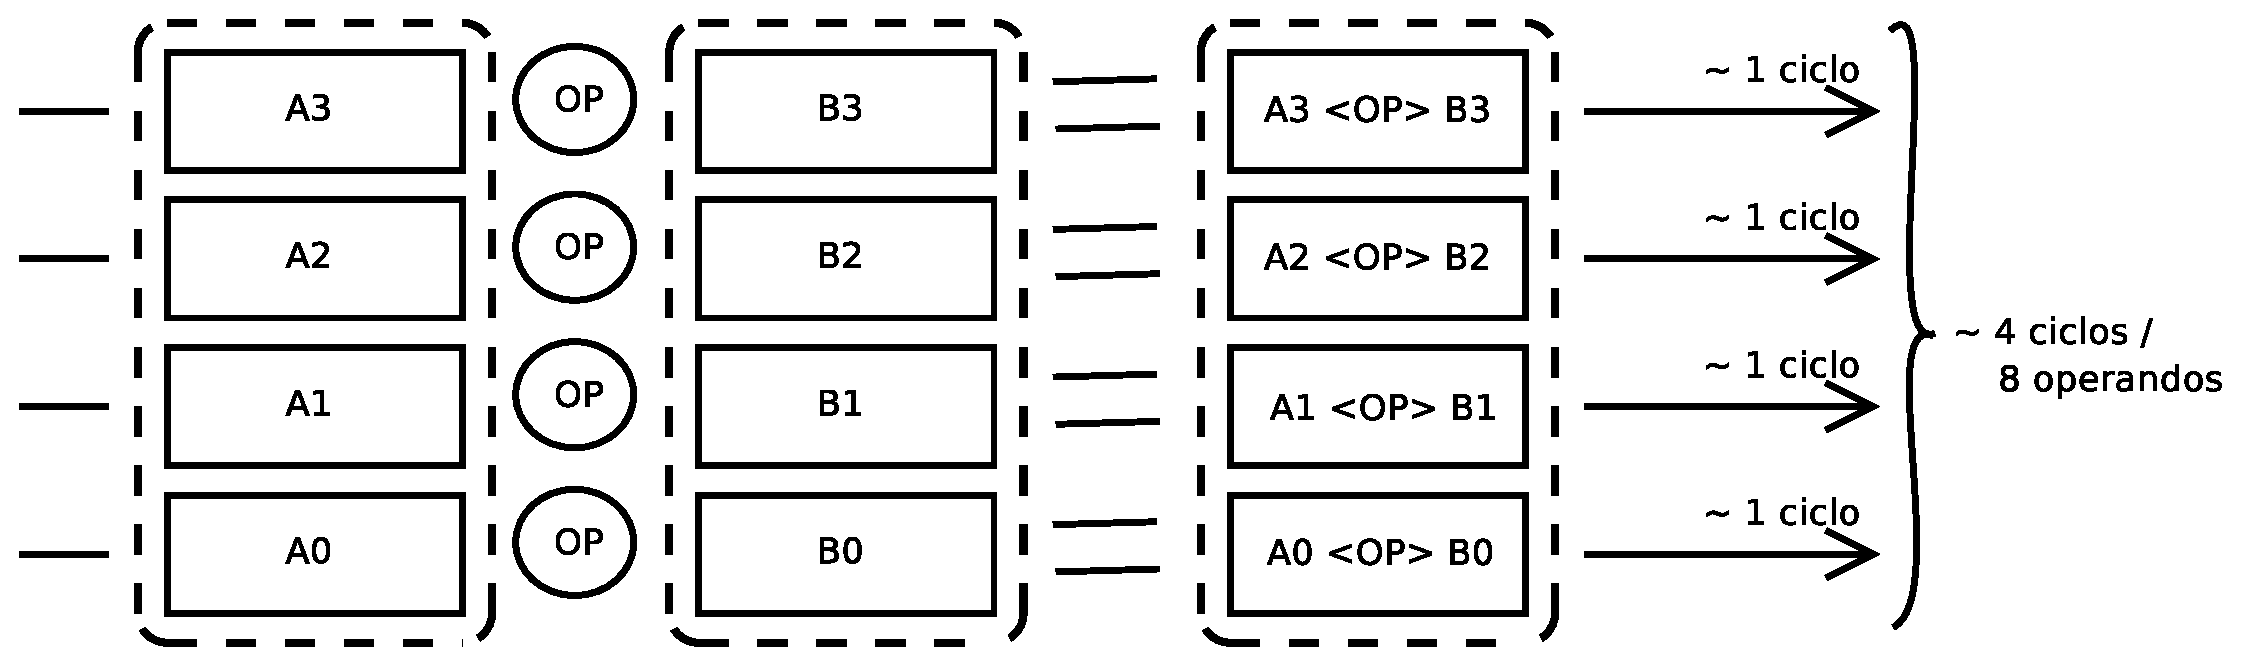
\includegraphics[width=0.85\textwidth,keepaspectratio]{sinSIMD} 
      \caption{Sin utilizar SIMD}\label{fig:sinSIMD}
    \end{figure}

    \begin{figure}[h]
      \centering
      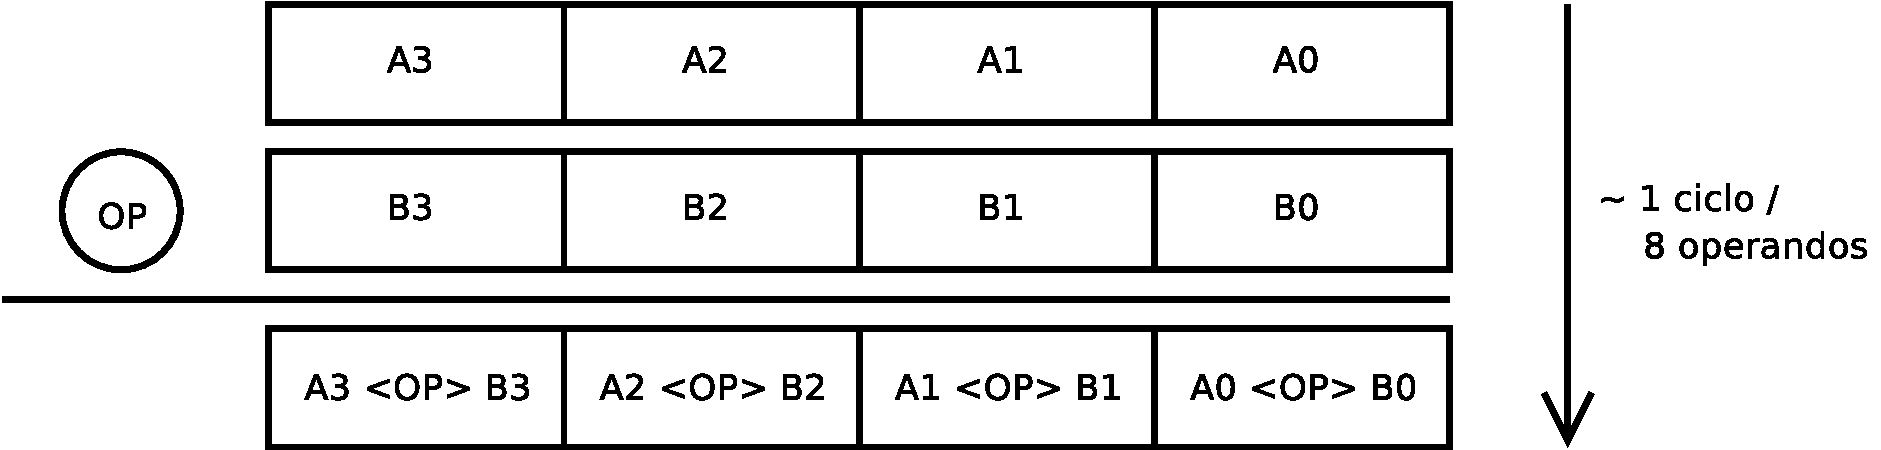
\includegraphics[width=0.85\textwidth,keepaspectratio]{conSIMD} 
      \caption{Utilizando SIMD}\label{fig:conSIMD}
    \end{figure}

    Este paralelismo intr�nseco al procesador requiere el uso de instrucciones espec�ficas del mismo, y es por ello
    dif�cilmente portable a otros sistemas. Asimismo, su utilizaci�n suele requerir el trabajo en lenguaje ensamblador, 
    con todo lo que ello supone (dificultad de mantenimiento, complejidad, etc.).

   La pr�ctica ubicuidad y potencia de estos m�todos los hacen muy atractivos. Con el fin de evitar el obst�culo
   de lo poco amigable de su uso, se ha desarrollado esta �CPU SIMD�. Sus objetivos son:
   \begin{itemize}
      \item Aislar a las rutinas de la biblioteca que deseen hacer uso de instrucciones SIMD de la implementaci�n
      real particular del procesador en cuesti�n sobre el que se est� operando. Incluso si no existe implementaci�n
      alguna, la biblioteca provee una implementaci�n gen�rica que simula su comportamiento.
      \item Homogeneizar la familia de operaciones disponibles, del mismo modo que se ha hecho con la CPU escalar.
      \item Proporcionar una abstracci�n adecuada que evite lidiar con los entresijos del lenguaje ensamblador. 
   \end{itemize} 

   \bigskip 

   Los �paquetes� SIMD tendr�n siempre una longitud de $128$ bits. En base a esto, se han definido
   tres variedades diferentes de �paquetes� de datos SIMD:
   \begin{itemize}
   \item Pares de n�meros en coma flotante de $64$ bits.
   \item Cuatro n�meros en coma flotante de $32$ bits.
   \item Ocho enteros con signo de $16$ bits.
   \end{itemize}
   Los detalles de la implementaci�n y una descripci�n m�s pormenorizada se dan en la secci�n \ref{simddigit}.



  \subsection{Repositorio de funciones}\label{basico:nuevoRepdeFuncs}
Ya en LibNumth exploramos la utilizaci�n de lo que se denomin� �repositorio de funciones�
(v�ase \cite{miproyecto}\footnote{secciones 5.6 y 4.2.3}). La idea era y sigue siendo
�hacer extensible la colecci�n de funciones \emph{sin necesidad de recompilaci�n} por parte del usuario,
y adem�s de forma sencilla�. La implementaci�n de este mecanismo en dicha versi�n de la biblioteca
era un tanto b�sica: depend�a de convenciones en el nombrado, haciendo recaer sobre el usuario
programador la carga de recordar el nombre concreto del tipo de funci�n que desease obtener. Por ejemplo:

\begin{lstlisting}[captionpos=b,basicstyle=\footnotesize,frame=shadowbox,rulesepcolor=\color{black},language=C++,numbers=left,caption=Utilizando el \textbf{antiguo} repositorio de funciones, label=lst:antiguoRepFuncs]
(...)
numth::Funciones funcs;

numth::congruentGen *LCG = new numth::congruentGen();
funcs.ponerRandom(LCG);

funcs.random()->ponerSemilla(numth::Z::convertir("323658476")); 
n = funcs.genPrimos()->leerPrimoProb(600);
(...)
\end{lstlisting}
En el anterior listado \ref{lst:antiguoRepFuncs} se aprecian los siguientes puntos:

\begin{itemize}
\item Tanto para establecer una nueva implementaci�n 
para una clase de m�todo, como para obtener la implementaci�n actual, era necesario estar al tanto del
nombre de la clase de m�todo que las instancias implementaban: \texttt{congruentGen} era un tipo de generador
de n�meros pseudo-aleatorios, y por ello deb�a utilizarse el m�todo \texttt{ponerRandom} de la clase \texttt{Funciones}, 
que representaba el repositorio. 
\item Para obtener un n�mero primo, el programador deb�a recordar que el m�todo
\texttt{genPrimos} era el indicado para obtener un puntero a una instancia generadora de primos. 
\item Incluso aunque se pretend�a seguir un patr�n de nombrado, �ste resultaba deficiente.
\item El repositorio, instancia de la clase \texttt{Funciones}, pod�a instanciarse de forma arbitraria, pese a que
conceptualmente el repositorio ha de ser �nico durante toda la ejecuci�n del programa. Este escollo se salvaba
haciendo que las instancias de las funciones contenidas en �l fueran \texttt{static}. Este simple hecho choca frontalmente
con el concepto de \textit{thread-safety}, tal como se expone en la secci�n \ref{par:datosStatic}.
\end{itemize}

Esta forma de operar no s�lo resulta tediosa y 
propensa a errores, sino tambi�n \emph{poco elegante}. La idea
es siempre que la m�quina trabaje por nosotros, no al contrario. Por si esto fuera poco, la presencia de datos
est�ticos da al traste con las aspiraciones de ejecuci�n concurrente de la biblioteca mediante hilos. 

Comparese el c�digo mostrado en el listado \ref{lst:antiguoRepFuncs} con el mostrado en el siguiente listado \ref{lst:nuevoRepFuncs}:
\begin{lstlisting}[captionpos=b,basicstyle=\footnotesize,frame=shadowbox,rulesepcolor=\color{black},language=C++,numbers=left,caption=Utilizando el \textbf{nuevo} repositorio de funciones, label=lst:nuevoRepFuncs]
(...)
mpplas::MethodsFactory& funcs(MethodsFactory::getReference());
mpplas::RandomFast* rnd;
mpplas::PrimeGen* primes;

mpplas::RandomFast* newRnd = new mpplas::CongruentGen();
funcs.setFunc(newRnd);

funcs.getFunc(rnd);
rnd->setSeed(mpplas::Z("323658476"));

funcs.getFunc(primes);
n = primes->getInteger(600);
(...)
\end{lstlisting}
Ambas porciones de c�digo son sem�nticamente equivalentes. Sin embargo:
\begin{itemize}
\item El repositorio, denominado ahora \texttt{MethodsFactory}, es ahora un \texttt{Singleton} (v�ase secci�n \ref{sec:singleton}). 
\item Se trabaja con punteros a los tipos que representan el concepto \emph{abstracto} a realizar: generar primos, obtener n�meros
pseudo-aleatorios, etc. en vez de con los tipos que en �ltima instancia implementan dichos conceptos.
\item El repositorio consiste \emph{�nicamente} de dos m�todos: \texttt{getFunc} y \texttt{setFunc}. El mecanismo
de funcionamiento, denominado \textit{autowiring}, se expone en \ref{sec:autowiring}. En este contexto, ambos
m�todos inspeccionan el tipo de las instancias que les son pasadas como par�metros a la hora de asignar
o establecer las instancias pertinentes, de forma totalmente transparente para el usuario, y garantizando \emph{en tiempo
de compilaci�n} la coherencia de dichas operaciones.
\end{itemize}

    
  \subsection{Control de errores}\label{controlDeErrores}


\section{Compilando la biblioteca}\label{estructuraGeneralDeLaLiberia}

% TECNOLOG�AS UTILIZADAS
\chapter{Tecnolog�as utilizadas}

\begin{flushright}
  \begin{minipage}[t]{13cm}
    \begin{flushright}
      \begin{quote}
        \emph{
          I've come up with a set of rules that describe our reactions to technologies:\\
            1. Anything that is in the world when you're born is normal and ordinary and is 
            just a natural part of the way the world works.\\
            2. Anything that's invented between when you're fifteen and thirty-five is new 
            and exciting and revolutionary and you can probably get a career in it.\\
            3. Anything invented after you're thirty-five is against the natural order of things.
        }
        \begin{flushright}
          \textbf{\textemdash Douglas Adams, The Salmon of Doubt}
        \end{flushright}
      \end{quote}
    \end{flushright}
  \end{minipage}
\end{flushright}

\bigskip



\begin{flushright}
  \begin{minipage}[t]{13cm}
    \begin{flushright}
      \begin{quote}
        \emph{
          Any sufficiently advanced technology is indistinguishable from magic.
        }
        \begin{flushright}
          \textbf{\textemdash Arthur C. Clarke, "Profiles of The Future" }
        \end{flushright}
      \end{quote}
    \end{flushright}
  \end{minipage}
\end{flushright}

\bigskip

\begin{center}{\line(1,0){325}}\end{center}

%--------------------------------------------------------%

\section{Comprobaciones en tiempo de compilaci�n}
%XXX: completar con una intro
  Siempre es mejor prevenir que curar, como reza el refranero. Por tanto, mejor que simplemente detectar el error
  cuando el programa ya se encuentra en ejecuci�n --que no es poco, pero no deja de ser una �mala cura�--, la detecci�n
  de condiciones que no deber�an darse es m�s efectiva cuanto antes se realice. La detecci�n en \emph{tiempo de compilaci�n}
  es el ideal, ya que estas comprobaciones no acarrear�an un incremento en tiempo de ejecuci�n\footnote{el tiempo de compilado
  s� es posible --incluso probable-- que aumente. Sin embargo, la compilaci�n es un proceso puntual, frente a un n�mero de ejecuciones
  arbitrario} y se detectar�an incluso antes de que el propio programa tomase cuerpo.

  Por otra parte, no es posible comprobar m�s que aquellas condiciones evaluables en tiempo de compilaci�n. En otras palabras,
  datos de car�cter \emph{constante} y \emph{est�tico}. En c�digo esto se traduce en valores declarados como \texttt{const static}, 
  o bien constantes --que no dejan de ser asimismo un caso particular de estos.

  
  \subsection{Asertos est�ticos}
  El concepto de \emph{aserto} como �comprobaci�n de la certeza de algo� en el mundo de la programaci�n
  se asocia habitualmente a comprobaciones \emph{en tiempo de ejecuci�n}. As�, por ejemplo, en C/C++ existe el mecanismo
  est�ndard \texttt{assert(ex)}, que interrumpir� la \emph{ejecuci�n} de un programa si su argumento \texttt{ex} se evalua como falso.
  Aunque pudiera parecer que las restricciones anteriormente descritas para las comprobaciones en tiempo de compilaci�n
  en general convierten en algo in�til el aserto est�tico, se expondr�n en el punto \ref{aplicacionesStaticAssert} 
  escenarios en los cuales s� resulta �til.

  Previamente, se mostrar� c�mo se consigue este comportamiento, 
  que no forma parte de C++ de forma directa. Consid�rese la macro mostrada en el listado \ref{lst::staticassert}.

\begin{lstlisting}[captionpos=b,basicstyle=\footnotesize,frame=shadowbox,rulesepcolor=\color{black},language=C++,numbers=left,caption=STATIC\_ASSERT, label=lst:staticassert]
#define STATIC_ASSERT(ex) \
  do { typedef int ai[(ex) ? 1 : -1]; } while(0) 
\end{lstlisting}

  Al contrario que en el caso del est�ndard \texttt{assert(arg)}, no interesa devolver un valor booleano: si la expresi�n
  a comprobar es falsa, el proceso de compilaci�n debe detenerse con un error. Si no lo es, continuar sin m�s. Idealmente,
  tampoco se generar� codigo adicional debido a estos asertos est�ticos.
  \texttt{STATIC\_ASSERT(ex)} se traduce mediante el preprocesador en una seria de sentencias un tanto particular:
  \begin{enumerate}
    \item Un bucle do-while que no itera ( \texttt{while(0)} nunca se evaluar� como cierto ).\label{enum:while0}
    \item Una declaraci�n de un alias de tipo mediante \texttt{typedef}. \label{enum:typedef}
    \item Dentro del punto anterior, una declaraci�n de un vector est�tico de un tama�o $1$ o $-1$ dependiendo
    de si \texttt{ex} resulta cierto o falso \emph{a ojos de C++}. \label{enum:elQuizStaticAssert}
  \end{enumerate}
  
  Previamente al an�sis de esta construcci�n: cuando se pone �nfasis en el valor de verdad \emph{a los ojos de C++},
  se quiere recordar al lector que, heredado del mundo de C, en C++ se evalua como cierto todo valor distinto
  de $0$\footnote{C++ contribuy� con el tipo \texttt{bool} y sus dos valores \texttt{true} y \texttt{false} a clarificar este �mbito,
  pero siguen siendo v�lidos los viejos h�bitos (y en este caso, necesarios)}.

  �Cumple con los requisitos anteriormente expuestos el c�digo anterior? Considerando su requisito fundamental, 
  que interrumpa la compilaci�n en funci�n de \texttt{ex}. Esto se consigue aprovechando la definici�n de 
  vector est�tico por parte del est�ndard ANSI C (\cite{c}\footnote{secci�n A8.6.2, p�g. 239}):
  \begin{quote}
  Si la expresi�n-constante est� presente, debe ser de tipo entero, y con valor mayor que $0$.
  \end{quote}
  Por �expresi�n-constante� se refiere en ese contexto al tama�o que se asigna al vector est�tico en su 
  declaraci�n. As� pues, por lo expuesto en el punto \ref{enum:elQuizStaticAssert}. de la enumeraci�n precedente,
  si \texttt{ex} se evalua como falso, se estar�a declarando \texttt{ai} con tama�o $-1$\footnote{�y por qu� si la
  referencia del lenguaje cita $0$ como valor ya invalido, se utiliza $-1$? Debido a que, tal como indica \cite{imperfectc++},
  por alguna raz�n algunos compiladores, entre ellos GCC y el compilador de Intel, s� consideran v�lido un vector est�tico de tama�o
  cero. Esto incumple claramente el est�ndard ANSI C, pero afotunadamente siquiera estos compiladores admiten un tama�o negativo
  como dimensi�n de dicho vector}, algo que incumple la sem�ntica de C, y por tanto, tambi�n de C++. Este incumplimiento resulta
  en una interrupci�n de la compilaci�n.

  La raz�n de ser de los puntos \ref{enum:while0}., y \ref{enum:typedef}. es la de no generar c�digo pero a la vez
  ser expresiones que s�n evaluadas por el compilador. Lo primero se consigue a ra�z de que en realidad no existe c�digo
  �ejecutable�, ninguna sentencia con efecto sobre el entorno. Cualquier compilador que realice optimizaci�n de c�digo (esto 
  es, todos) omitir� incluir ninguna instrucci�n correspondiente a esta porci�n de c�digo. Pero no antes de haberla evaluado:
  a ra�z de que el bucle, al ser do-while, fuerza la entrada en su cuerpo al menos una vez. En este cuerpo, el \texttt{typedef}
  ha de evaluar el nuevo alias declarado: el vector est�tico en cuya dimensi�n reside el meollo de la cuesti�n.

  V�ase \cite{imperfectc++}\footnote{secci�n 1.4.8, p�g. 25} para un enfoque de este m�todo en m�s en profundidad.

    \subsubsection{Aplicaciones}
    %TODO

  \subsection{Pruebas de paternidad}
  El siguiente m�todo para asegurarse que una clase dada hereda de otra se expone en 
  \cite{imperfectc++}\footnote{secci�n 1.2.1, p�g. 5}. Su utilidad, una vez m�s, deriva del hecho de ser
  una comprobaci�n \emph{en tiempo de compilaci�n}


  Ver un ejemplo de la utilizaci�n de este patr�n ayudar� a explicar el funcionamiento del mismo. Consid�rese
  el listado \ref{lst:musthavebaseEj}. 
  \lstset{escapeinside={(*@}{@*)}}
  \begin{lstlisting}[captionpos=b,basicstyle=\footnotesize,frame=shadowbox,rulesepcolor=\color{black},language=C++,numbers=left, caption=Ejemplo de uso del patr�n de verificaci�n de paternidad, label=lst:musthavebaseEj]
Constraints::must_have_base<S, Ring<S> > dummy1; (*@\label{algparent:Ring}@*)
Constraints::must_have_base<S, MPPDataType > dummy2; (*@\label{algparent:MPPDataType}@*)
  \end{lstlisting}
  Este trozo de c�digo se corresponde a la clase \texttt{Polynomial<S>} (v�anse las secciones \ref{tipos:polinomios} 
  y \ref{impl:polinomios} para una descripci�n de este tipo de dato y una pormenorizaci�n de sus detalles de 
  implementacion, respectivamente). En la l�nea \ref{algparent:Ring} se comprueba que el tipo de plantilla S 
  --que recordemos se corresponde al tipo de los coeficientes del polinomio-- 
  \ref{algparent:MPPDataType} 

  El c�digo implementando el patr�n de comprobaci�n de paternidad se muestra en el listado \ref{lst:musthavebase}.
  \begin{lstlisting}[captionpos=b,basicstyle=\footnotesize,frame=shadowbox,rulesepcolor=\color{black},language=C++,numbers=left, caption=Verificaci�n de paternidad en tiempo de compilaci�n, label=lst:musthavebase]
template<typename D, typename B>
struct must_have_base{
  ~must_have_base(){
    void(*p)(D*, B*) __attribute__ ((__unused__)) = constraints;
  }
  private:
  static void constraints(D* pd, B* pb){
    pb = pd;
  }
}; 
  \end{lstlisting}


    \subsubsection{Aplicaciones}
    %TODO

\section{Programaci�n orientada a aspectos (AOP)}

\section{Mix-ins}

\section{Mock objects}

\section{Test units}
 



% TIPOS SOPORTADOS POR LA BIBLIOTECA
\chapter{Tipos soportados}\label{chap:tipos}

\begin{flushright}
  \begin{minipage}[t]{13cm}
    \begin{flushright}
      \begin{quote}
        \emph{
          It turns out that an eerie type of chaos can lurk just behind a
          facade of order -- and yet, deep inside the chaos lurks an even
          eerier type of order.
        }
        \begin{flushright}
          \textbf{\textemdash Douglas Hostadter}
        \end{flushright}
      \end{quote}
    \end{flushright}
  \end{minipage}
\end{flushright}

\bigskip

\begin{flushright}
  \begin{minipage}[t]{13cm}
    \begin{flushright}
      \begin{quote}
        \emph{
          God is Real, unless declared Integer
        }
        \begin{flushright}
          \textbf{\textemdash J. Allan Toogood}
        \end{flushright}
      \end{quote}
    \end{flushright}
  \end{minipage}
\end{flushright}

\begin{center}{\line(1,0){325}}\end{center}

%--------------------------------------------------------%

\section{Introducci�n}
En la figura \ref{fig:jerarquiaTipos} se muestran los distintos tipos soportados por la biblioteca y una
visi�n general de sus interrelaciones. 
  \begin{figure}[h]
    \centering
    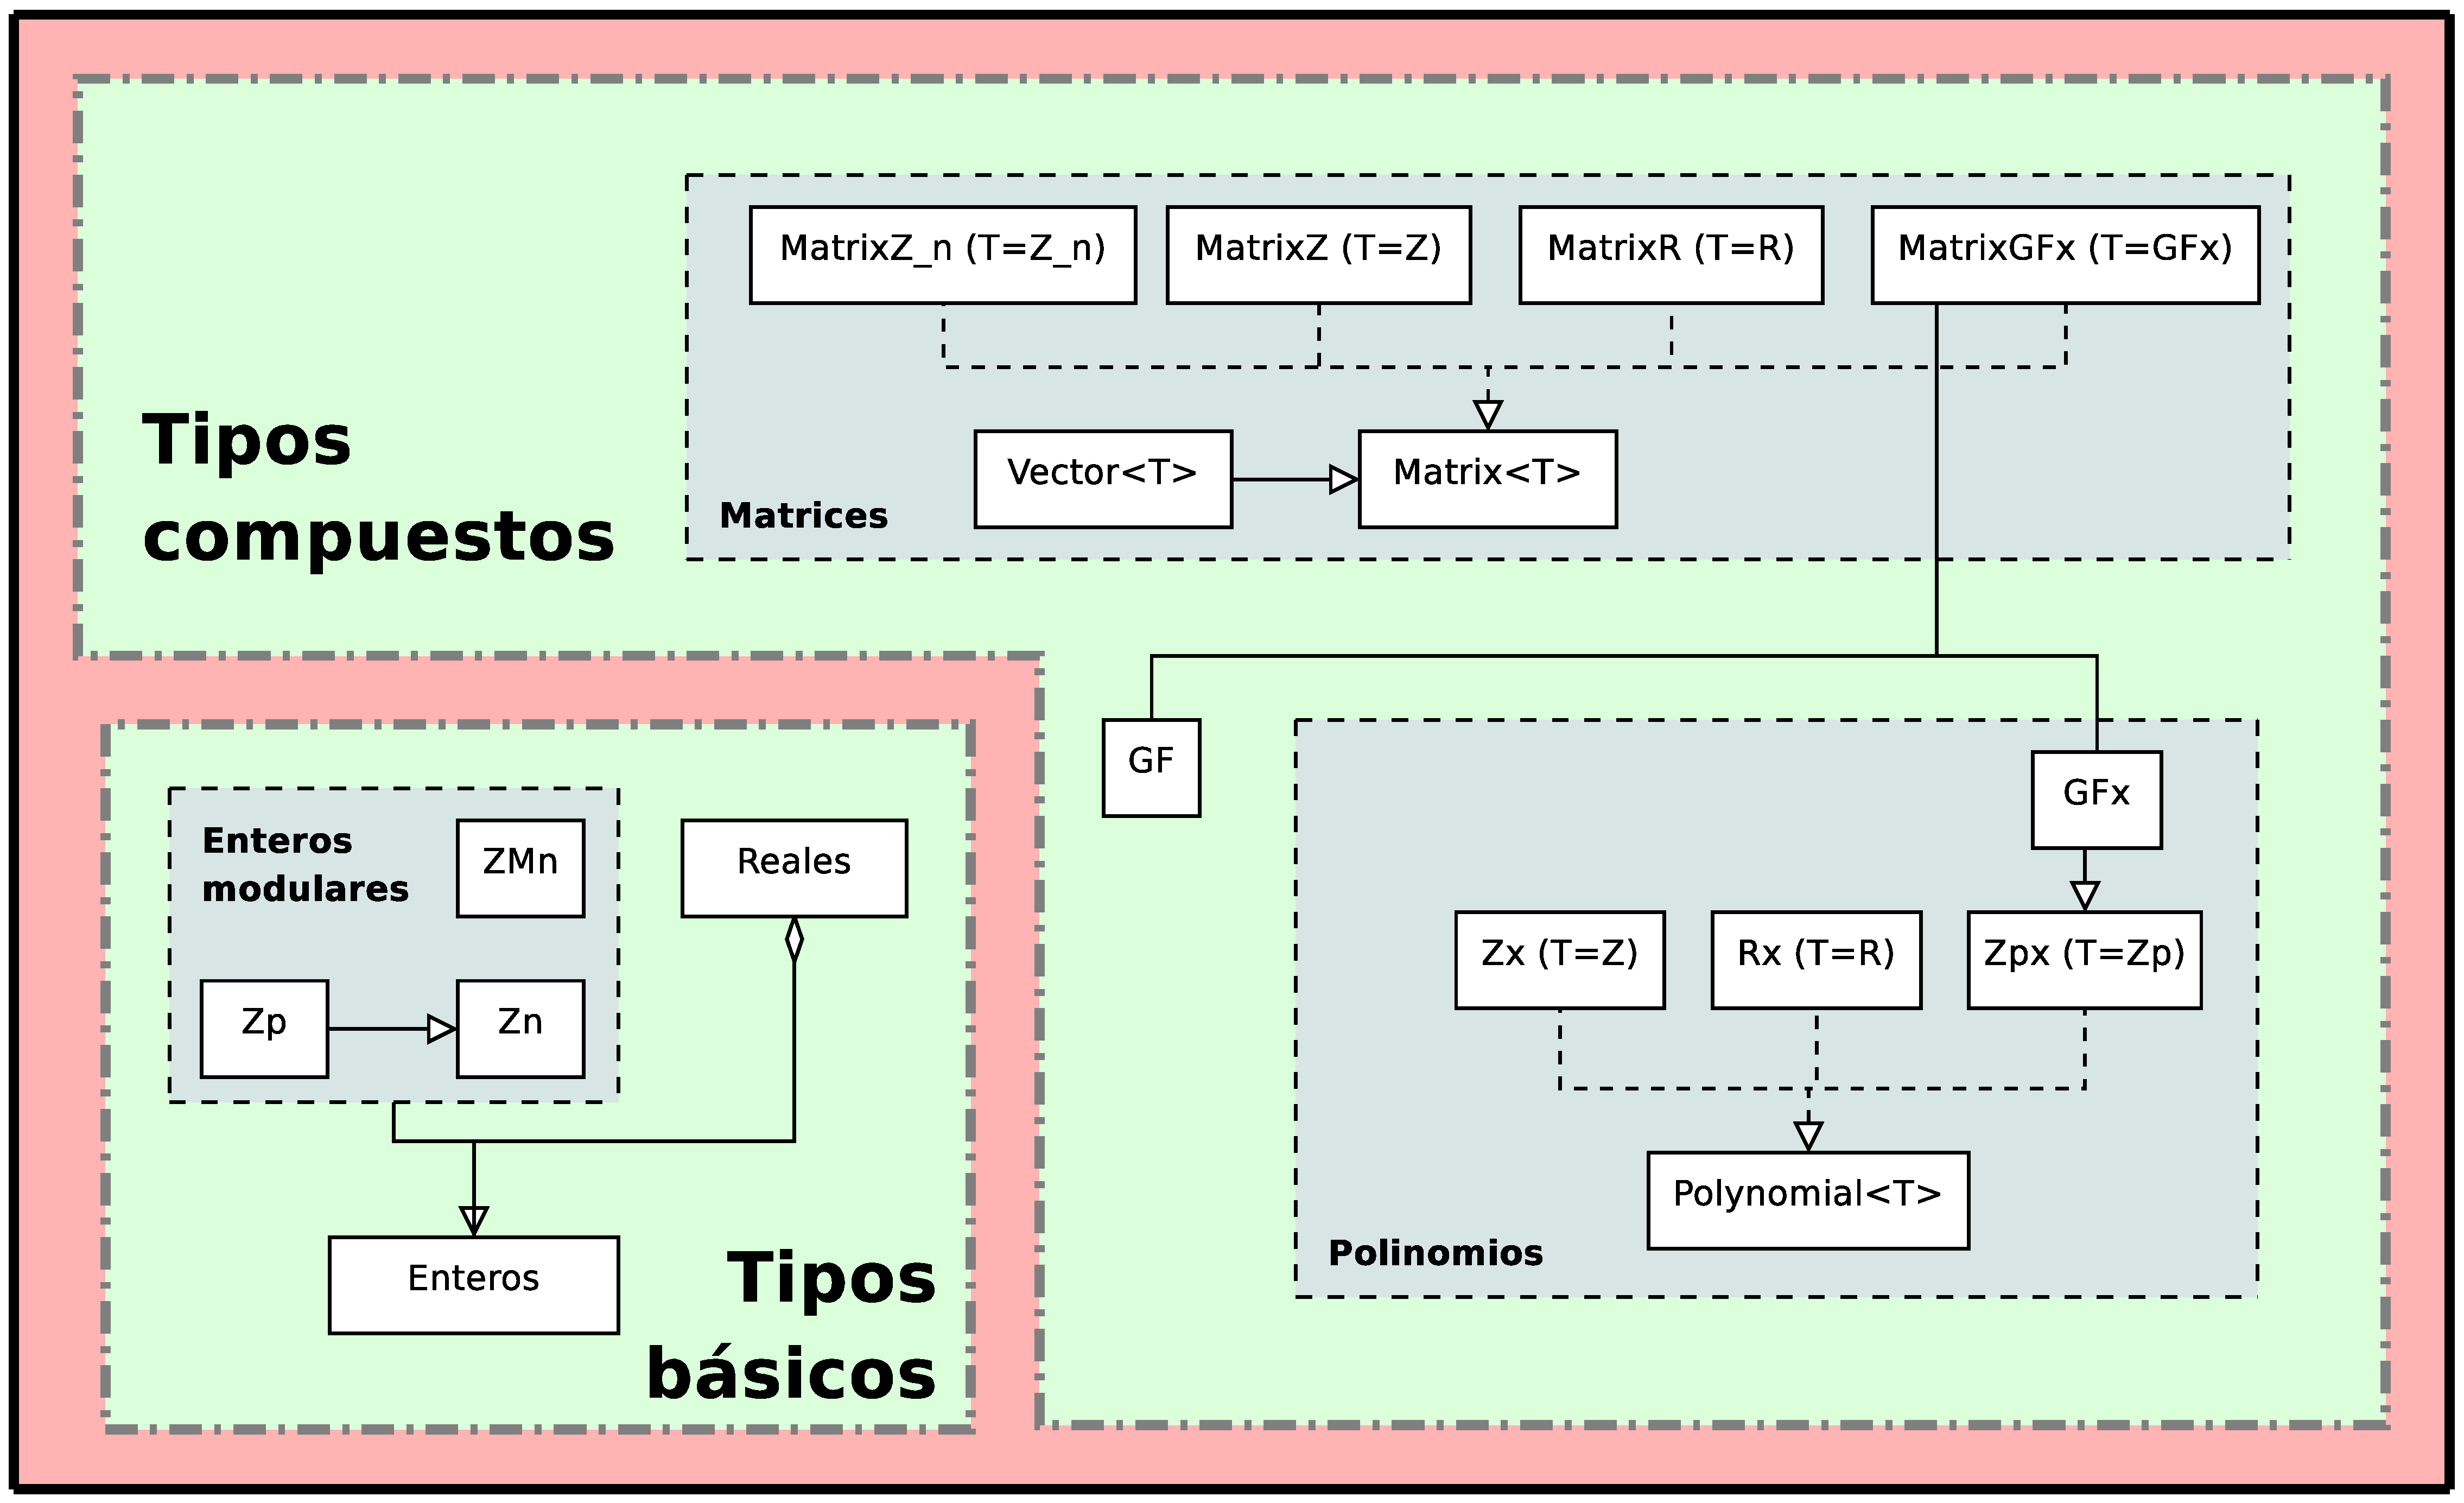
\includegraphics[width=0.95\textwidth,keepaspectratio]{jerarquiaTipos} 
    \caption{Tipos de la biblioteca}\label{fig:jerarquiaTipos}
  \end{figure}
Los tipos denominados compuestos, las matrices y los polinomios, reciben un tipo
como argumento de plantilla: el tipo de sus elementos. Este concepto de tipo de
plantilla es, claro est�, propio de C++, no de la biblioteca. Sin embargo, como se
expone en detalle en \ref{categorizacionAlgebraica}, se han incorporado mecanismos 
para asegurar que la coherencia matem�tica se mantenga. Tambi�n en dicha secci�n, 
concretamente en la figura \ref{fig:categoriasAlgebraicas}, se presenta el modo en el que
para cada tipo se ha modelado su categor�a algebraica. 

Respecto a LibNumth, la familia de tipos disponibles ha aumentado cuantitativa y cualitativamente.
No s�lo se han a�adido tipos completamente nuevos, sino que se han refinado los ya presentes. Por ejemplo,
el cuerpo $\mathbb{Z}_p$ que antes pod�a modelarse �nicamente mediante $\mathbb{Z}_n$ con un $n$ primo, ahora cuenta
con tipo propio, lo que permite sacar partido de sus caracter�sticas particulares como cuerpo: $\mathbb{Z}_n$ s�lo
puede ser considerado como anillo si no se imponen restricciones sobre el m�dulo $n$.


\section{El tipo general \texttt{MPPDataType}}\label{tipos:mppdatatype}
Formalmente, no es un tipo \emph{de dato}. Es m�s bien un tipo abstracto del cual todos los 
dem�s tipos de la biblioteca, directa o indirectamente, heredan. De hecho, la definici�n de
�tipo de la biblioteca� podr�a ser �todo tipo que tenga a \texttt{MPPDataType} como ancestro�.
�Qu� ventajas aporta el contar con un tipo padre �nico? La experiencia de lenguajes orientados 
a objeto que --a diferencia de C++-- s� cuentan con un tipo de dato gen�rico ancestro com�n de
todos los dem�s demuestra que resulta efectivamente �til: por ejemplo, Java cuenta con la clase \texttt{Object},
lo cual permite por una parte definir m�todos comunes para todas las dem�s clases, as� como
poder declarar colecciones �gen�ricas�. 

En la biblioteca, se explota la primera de estas caracter�sticas: el definir m�todos comunes 
a todos los tipos. En concreto, y copiando a Java flagrantemente, se define como m�todo virtual
puro \texttt{std::string toString()}, que devuelve una representaci�n textual del dato. 
El siguiente c�digo es por tanto v�lido para copiar un entero:

\begin{lstlisting}[captionpos=b,basicstyle=\footnotesize,frame=shadowbox,rulesepcolor=\color{black},language=C++,numbers=left,caption=Uso de \texttt{toString()}]
  Z n("123");
  Z m( n.toString() );
  
  // n == m
\end{lstlisting}
  
�Para qu� hacer esto cuando se puede utilizar directamente el constructor de copia del dato? Desde luego
en situaciones en las que se tenga acceso a la \emph{instancia} del dato a ser copiado, es absurdo hacerlo 
de la forma anterior. Sin embargo, si nos encontramos con un escenario distribuido, no es trivial \textit{serializar}
\footnote{es decir, transformar una instancia arbitraria en una representaci�n �nicamente basada en tipos b�sicos 
susceptible de ser transferida a trav�s de la red} una instancia de un dato arbitrario. Sin embargo s� es inmediato
serializar una cadena de caracteres. Si mediante la representaci�n textual es posible reproducir la instancia en cuesti�n,
se habr� salvado este obst�culo.

La segunda y �ltima funci�n virtual pura declarada en el tipo \texttt{MPPDataType} es \texttt{std::string toHRString()}, en la
que �HR� corresponde a �\textit{Human Readable}�: la idea es devolver una representaci�n textual susceptible de ser mostrada
a un usuario humano. En algunos casos la representaci�n ser� la misma que la devuelta
por \texttt{toString()} --tal como en el caso de los enteros--, mientras que en otros ser� diferente --para las matrices, 
por poner un caso--.

\bigskip

Poder declarar \emph{colecciones gen�ricas}, tales como un vector que almacene cualquier tipo de dato soportado
por la biblioteca, resulta extremadamente �til a la hora de programar de forma gen�rica. Un ejemplo de esto 
se encuentra en la implementaci�n de los mecanismos de gesti�n de datos en tiempo de ejecuci�n del entorno de ejemplo
desarrollado, el cual se describe en la secci�n \ref{par:runtimeData}.

%Enteros, Z
\section{Enteros}
  La base de los dem�s tipos, ya sea por herencia o composici�n; es decir, formando un subconjunto --como en el caso 
  de $\mathbb{Z}_n$-- o siendo utilizados internamente en las representaciones --como en $\mathbb{R}$--. El grueso 
  de su implementaci�n base proviene de LibNumth. Sin embargo se han realizado optimizaciones y a�adido algunos m�todos
  en esta nueva versi�n de la biblioteca. %TODO: cuales?

\section{Enteros modulares}
  En Teor�a de N�meros, y por extensi�n en criptograf�a, se utilizan con mucha frecuencia enteros modulares. 
  Pese a que forman un subconjunto de los enteros, y que toda operaci�n sobre un entero modular puede reducirse
  en �ltima instancia a operaciones sobre los enteros habituales, es posible aprovecharse de sus caracter�sticas
  particulares. Esto justifica su modelado por separado. 
  %TODO

  \subsection{Enteros m�dulo un primo}
    Si en $\mathbb{Z}_n$ se restringe el m�dulo $n$ a n�meros primos, es un resultado b�sico en Teor�a de N�meros %TODO: cita
    que la estructura algebraica resultante, usualmente denominada $\mathbb{Z}_p$, tiene car�cter de \emph{cuerpo}. 
    Esto es, se garantiza la existencia de inversa para todo elemento no nulo. La relevancia de esta estructura
    en Teor�a de N�meros es muy grande. %TODO: aplicaciones

    La biblioteca modela a esta estructura de forma independiente, no como un mero caso particular de $\mathbb{Z}_n$, sacando
    partido de los mecanismos de categorizaci�n algebraica de la misma. 

  \subsection{Enteros modulares en el dominio de Montgomery}\label{sec:zm}
  Nombrados como $\mathbb{Z}M_n$, son un tipo de entero modular, siendo
  su m�dulo reductor $n$. Su particularidad estriba en que ninguna de sus
  operaciones requiere el uso de la divisi�n, excepto en el caso de potencias
  de la base de trabajo, operaci�n que se realiza mediante desplazamientos.
    
  Hasta donde se tiene constancia, se trata de un tipo de dato original
  de esta biblioteca: no se tiene conocimiento de su implementaci�n en otras bibliotecas
  similares. 

  \subsubsection{Preliminares}
  Una conocida forma de exponenciaci�n modular se basa en el m�todo de
  multiplicaci�n/reducci�n de Montgomery (\cite{montgomeryOrig}). 
  El m�todo de reducci�n-multiplicaci�n se encontraba ya incorporado en
  la antigua versi�n de la biblioteca (v�ase \cite{miproyecto}\footnote{secci�n 5.5.3}),
  utiliz�ndose precisamente para la exponenciaci�n modular. 

  A lo largo de esta secci�n se utilizar� la nomenclatura introducida en \cite{miproyecto}\footnote{secci�n 5.2}, para 
  los siguientes conceptos: $B$ representa la base con la que la m�quina trabaja
  internamente de forma �ptima, en la que se representan los tipos de datos b�sicos \texttt{Digit}.
  El n�mero de bits de esta base se denominar� $BED$: bits en \texttt{Digit}. La implementaci�n actual
  soporta valores de $BED$ de $32$ y $64$.

  Mediante la precomputaci�n de dos valores, 
  $R_n = 2^{i\cdot BED} \mid i \in \mathbb{Z}, i \geq 1$ y $-n^{-1} \pmod{BED}$, 
  resulta posible prescindir de la operaci�n de divisi�n. 
  Dichos valores dependen �nicamente del m�dulo $n$, por lo que si se realizan muchas
  operaciones con el mismo m�dulo, el coste computacional de su c�lculo se ve compensado
  por la ausencia de divisiones. 

  Anteriormente no se ha especificado ning�n valor para la $i$ en
  $R_n = 2^{i \cdot BED}$. Seg�n \cite{handbook}\footnote{p�g. 600}, es suficiente con que se verifique 
  $R > n$. Ahora bien, consid�rese la longitud del m�dulo $n$ en la base de trabajo $B$ definida con anterioridad
  como $k$. Es posible concluir entonces 
  \begin{equation}
  R_n = 2^{k \cdot BED} = B^{k} \Rightarrow i = k \label{eq:defRMont}
  \end{equation}
  Esto simplifica e incrementa el rendimiento de las operaciones,
  tal como se indica en  \cite{handbook}\footnote{Fact 14.30 (ii), p�g. 601}. Sin embargo, la limitaci�n que esto
  impone es la imposibilidad de utilizar un m�dulo $n$ par. De todas maneras, en los escenarios de aplicaci�n m�s comunes
  $n$ es primo.

  Un concepto fundamental en esta discusi�n es el de \emph{dominio de Montgomery}.
  \begin{definicion}[Dominio de Montgomery]
  Se considera que $a \in \mathbb{Z}$ pertenece al \emph{dominio de Montgomery} para
  un m�dulo $n$ si $a < n$ y $R_n | a$, esto es, si $a$ es m�ltiplo de $R_n$.
  \end{definicion}
  Las operaciones habituales de suma, resta, producto, divisi�n (como combinaci�n de inversi�n m�s producto) 
  en este dominio est�n bien definidas, como se expone en la secci�n \ref{opsZM}.


  \subsubsection{Operaciones}
  Las operaciones sobre $\mathbb{Z}M_n$ se dividen en dos grupos:
  las orientadas al trabajo dentro del propio dominio, denominadas �espec�ficas�, 
  y las que se corresponden con las operaciones habituales sobre $\mathbb{Z}$, 
  denominadas �habituales�, presentadas de cara al usuario programador.

  \paragraph{Espec�ficas.}
  \begin{definicion}[Multiplicaci�n de Montgomery]\label{def:multMont}
  Sea $R_n$ tal como se define en la expresi�n \eqref{eq:defRMont}, $x,y \in \mathbb{Z}$. 
  Se define la funci�n \texttt{MultMon} como
  \[
    \mathtt{MultMon}(x,y,n) = x \cdot y \cdot R^{-1} \pmod{n}
  \]
  \end{definicion}


  \begin{definicion}[Inversa de Montgomery (\cite{kaliski})]\label{def:invMont}
  \[
    \mathtt{InvMon}(a,n) = a^{-1} \cdot R \pmod{n}
  \]
  \end{definicion}


  Ko� y Savas (\cite{montInvRev}) ampliaron el
  concepto, en especial con una �nueva inversa de Montgomery�:
  \begin{definicion}[Inversa de Montgomery (\cite{montInvRev})]\label{nuevaMontInv}
  Sea $R_n$ tal como se define en la expresi�n \eqref{eq:defRMont}, $a \in \mathbb{Z}$. 
  \[
    \mathtt{NuevaInvMon}(a \cdot R,n) = a^{-1} \cdot R \pmod{n}
  \]
  \end{definicion}
  Es decir, este �ltimo m�todo obtiene la inversa de un n�mero dado en el
  dominio de Montgomery, manteni�ndose tambi�n el resultado en dicho dominio.

  \paragraph{Habituales.}\label{opsZM}
  A continuaci�n se definen las operaciones b�sicas sobre este tipo 
  de enteros modulares en el dominio de Montgomery, as� como la conversi�n
  hacia y desde $\mathbb{Z}$ � $\mathbb{Z}_n$.

  En lo sucesivo se asume que los operandos comparten el mismo m�dulo
  $n$.

  \subparagraph{Suma y resta} 
  Sean $x,y \in \mathbb{Z}_n$,
  $0 \le xR, yR < n  \Rightarrow  xR + yR = (x+y)R \leq 2n-2$
  con lo que si la suma es mayor que $n$, bastar� con restar $n$ a �sta a lo sumo una vez.

  Para la resta, el razonamiento es an�logo, salvo que en este caso, el m�dulo habr� de
  sumarse si $(x-y)R < 0$, a lo sumo dos veces.

 \subparagraph{Producto} 
  Utilizando la multiplicaci�n de Montgomery (v�ase la definici�n \ref{def:multMont}),
  se obtiene el producto de dos elementos del dominio de Montgomery, resultando 
  su producto tambi�n en �ste, de la siguiente manera:
  $\mathtt{MultMon}( xR, yR ) = xR \cdot yR \cdot R^{-1} = xyR^2 \cdot R^{-1} = xyR$

  \subparagraph{C�lculo de la inversa}
  Aplicar $\mathtt{NuevaInvMon}$ directamente (v�ase la definici�n \ref{nuevaMontInv}).
  \subparagraph{Divisi�n}
    La divisi�n se realiza mediante las operaciones de inversi�n y producto: 
    $ (aR / bR ) = \mathtt{MultMon}( aR, b^{-1}R )$. A su vez, 
    $ \mathtt{MultMon}( aR, b^{-1}R ) = aR \cdot b^{-1}R \cdot R^{-1} = ab^{-1}R $
 
 \subparagraph{Conversi�n desde $\mathbb{Z}$ a $\mathbb{Z}M_n$}
  Si el entero a convertir verifica $a \geq n$, se realizar  previamente una reducci�n m�dulo $n$.
  Dado $0 \leq a < n$ , $\mathtt{MultMon}( a, R^2, n ) = a R^2 R^{-1} \pmod{n}  = a \cdot R \pmod{n}$

  \subparagraph{Conversi�n desde $\mathbb{Z}M_n$ a $\mathbb{Z}$}
   Dado $0 \leq aR < n$ , $\mathtt{MultMon}( aR, 1, n ) = a R \cdot 1 \cdot R^{-1} \pmod{n} = a \pmod{n}$
   N�tese que el entero $a$ resultante se devuelve reducido m�dulo $n$, con lo que encajar�a tambi�n 
   dentro de $\mathbb{Z}_n$ sin necesidad de una nueva reducci�n modular.


  \subsubsection{Aplicaciones}
  El utilizar este tipo hace que trabajar en $\mathbb{Z}_n$ sea mucho m�s r�pido.
  Esto es debido a que, como se ha mencionado anteriormente, 
  no se realizan divisiones --el �algoritmo b�sico�\footnote{
  la divisi�n \emph{no} es una operaci�n b�sica como err�neamente 
  suele considerarse. Tan solo la suma y el producto (para las estructuras
  algebraicas donde tuviera lugar) lo son.}
   computacionalmente
  m�s costoso. Asimismo, el c�lculo del elemento inverso a uno dado
  no requiere del uso del algoritmo extendido de Euclides 
  (v�ase \cite{miproyecto}\footnote{secci�n 5.5.2, p�g. 64}),
  tambi�n computacionalmente costoso. 

  Ahora bien, la creaci�n y conversi�n desde/hacia los enteros habituales es costosa. 
  Resulta conveniente mantenerse en el dominio de Montgomery durante el mayor n�mero de
  operaciones posibles. Determinados algoritmos se prestan a esto: aquellos en los que
  el m�dulo de trabajo es com�n a un cierto n�mero de operaciones, donde se utilicen
  frecuentemente exponenciaciones e inversiones. Dos ejemplos de algoritmos tales son
  el mecanismo de firma digital DSA (\cite{schneier}\footnote{secci�n 20.1, p�g. 483}) 
  y el mecanismo de firma y cifrado ElGamal (\cite{schneier}\footnote{secci�n 19.6, p�g. 476}).

  %TODO
  %En la secci�n \ref{ejZM_n} se recoge una comparativa de la implementaci�n de estos m�todos 
  %mediante datos en $\mathbb{Z}_n$ y $\mathbb{Z}M_n$.


\section{Reales}
  Realizando una analog�a quiz�s poco rigurosa pero ilustrativa, los reales son al C�lculo Num�rico 
  como los enteros a la Teor�a de N�meros: conforman su tipo base fundamental. Respecto a su anterior
  implementaci�n en \cite{miproyecto}, se han optimizado internamente sus m�todos y a�adido nuevas operaciones, 
  describiendose a continuaci�n algunas de las m�s relevantes.
  
  \subsection{C�lculo de la ra�z cuadrada}\label{tipos:sqrt}
  La funci�n $\sqrt{A}$, puede definirse como las ra�ces de la funci�n $f(x) = x^2 - A$. Esto lleva a pensar
  inmediatamente en la utilizaci�n de un m�todo iterativo para el c�lculo de ra�ces. Por ejemplo, el conocido
  m�todo de Newton --descrito por ejemplo en \cite{recipes,calculoburgos}\footnote{secci�n 9.4, p�g. 366; secci�n 092, p�g. 
  258, resp.}--, lo que nos llevar�a a la siguiente formulaci�n:
  \begin{eqnarray}
   x_{n+1} & = & x_n - \frac{f(x_n)}{f'(x_n)} =  \nonumber \\
           & = & \frac{1}{2} \left( x_n + \frac{A}{x_n}  \right) \label{newtonDiv}
  \end{eqnarray}
  
  Este m�todo es eficaz, tanto en cuanto devuelve efectivamente un resultado correcto para $\sqrt{A}$. 
  Sin embargo, adolece de un problema desde el punto de vista del rendimiento en la pr�ctica: en la
  expresi�n \eqref{newtonDiv}, se requiere realizar la divisi�n $A / x_n$ en cada paso. 

  Con un peque�o ajuste (\cite{sqrt}) es posible evitar esta divisi�n y realizar solamente multiplicaciones, con la 
  consiguiente mejora de rendimiento. Consid�rese la funci�n $f(x) = 1/x^2 - A$, es decir, el c�lculo
  de la inversa de la ra�z cuadrada, $1/\sqrt{A}$. En este caso,
  \begin{equation}
    x_{n+1} = \frac{3}{2} x_n - \frac{1}{2}Ax_n^3 \label{newton2}
  \end{equation}

  Como se ha dicho, esta iteraci�n converge a $1/\sqrt{A}$. Multiplicando este valor por $A$, se 
  obtiene el deseado valor de $\sqrt{A}$.

  La iteraci�n definida en \eqref{newton2} tiene convergencia cuadr�tica. Es posible ir mas all�. Por ejemplo,
  en \cite{sqrt} se aplica el m�todo de Newton dos veces, lo cual resulta en una convergencia cu�druple:

  \begin{equation}
  x_{n+1} = x_n - \frac{x_n}{16}(1-Ax^2_n)(-20 + 19A x^2_n - 8A^2 x^4_n + A^3 x^6_n) \label{newton3}
  \end{equation}

  Pero una vez m�s, todav�a puede mejorarse. Dada la regularidad de $f$, resulta posible aplicar
  una variante tambi�n cu�druple del m�todo de Newton dada en \cite{newton}\footnote{secci�n 4.2}:
  
  \begin{equation}
  x_{n+1} = x_n - \frac{x_n}{16}(1-Ax^2_n)(-19 + 16Ax^2_n - 5A^2 x^4_n) \label{newton4}
  \end{equation}

  Si se comparan las expresiones \eqref{newton3} y \eqref{newton4}, vemos como la segunda
  resulta computacionalmente m�s sencilla de evaluar dado el menor orden del polinomio
  que contiene, a�n manteniendo su orden de convergencia. Reformulando:

  \begin{equation}
  \left\{ 
    \begin{array}{l}
      h_n = 1 - Ax^2_n \\
      x_{n+1} = x_n + \frac{x_n}{16} \left(  8h_n + 6h^2_n +5h^3_n \right) \label{eq:sqrtFinal}
    \end{array} 
  \right.
  \end{equation}


  V�ase la secci�n \ref{impl:sqrt} para detalles espec�ficos de la implementaci�n.

  \subsection{Funciones trascendentes}
    Se define como \emph{transcendente} toda funci�n no algebraica. En otras palabras,
    que no puede expresarse en t�rminos algebraicos. Su denominaci�n deriva del hecho
      de �trascender� al �lgebra.

      Se han incorporado a la biblioteca m�todos para el c�lculo de las siguientes
      funciones trascendentes.
    \begin{description}
      \item[Exponencial.] Operaci�n representada usualmente como $exp(x) = e^x$, siendo 
       $e$ la base de los logaritmos neperianos. Esta funci�n, antiguamente denominada como
       �la e-funci�n de Euler� (\cite{oxfordmath}\footnote{p�g. 51}), tiene el siguiente valor:
       $exp(1) = e = 1 + 1 + \frac{1}{2!} + \frac{1}{3!} + \cdots \approx 2.7182\ldots$. 
       Esta constante $e$ encierra muchas otras sorpresas, siendo b�sica en el estudio 
       del cuerpo de los n�meros complejos. Se combina con otras dos c�lebres constantes en la
       conocida y sorprendente, a primera vista, expresi�n $e^{i \pi} = -1$.
      \item[Logaritmo neperiano.] Operaci�n inversa a la exponencial, para $y = \ln{(x)}$,
        se verifica $e^y = x$. N�tese que el c�lculo del logaritmo en otra base $b$
          distinta de $e$ se reduce a: $\log_b{(x)} = \ln{(x)} / \ln{(b)}$.
      \item[Funciones trigonom�tricas.] Es decir, las funciones seno y coseno, as� como las
      definidas a partir de �stas, como la tangente. 
    \end{description}

    \subsubsection{C�lculo de $\pi$}
      El c�lculo de la proporci�n entre la longitud y di�metro de la circunferencia, m�s
      conocida como $\pi$, es un c�lculo cl�sico utilizado habitualmente como prueba
      ya sea de rendimiento o de correcto funcionamiento por parte de bibliotecas o paquetes
      de c�lculo num�rico. En el caso que nos ocupa no se ha pretendido realizar una implementaci�n
      que vaya a batir marcas de rendimiento, sino m�s bien implementar uno mismo uno de los muchos
      m�todos disponibles para el c�lculo de una de las constante m�s famosas.

      

\section{Polinomios}\index{tipos!Polinomios}\label{tipos:polinomios}
  En \cite{knuth}\footnote{p�g. 418} se define polinomio como:

  \begin{definicion}[Polinomio]
    Un \emph{polinomio sobre \texttt{S}} es una expresi�n de la forma
    \begin{equation}
    u(x) = u_n x^n + \cdots + u_1 x + u_0 \label{poly}
    \end{equation}
    donde los \emph{coeficientes} $u_n,\ldots,u_1,u_0$ son elementos de alg�n
    sistema algebraico \texttt{S}, y la \emph{variable} $x$ puede ser considerada como 
    un s�mbolo formal con un valor indeterminado.

    N�tese que se considera al polinomio $0x^{n+m}+\cdots+0x^{n+1} + u_nx^n + \cdots + u_1x+u_0$ 
    equivalente a \eqref{poly}.

    Se define el \emph{grado} del polinomio \eqref{poly} como $n$, y su \emph{coeficiente director}
    como $u_n (\neq 0)$.

    Se denomina \emph{polinomio m�nico} al polinomio cuyo coeficiente director es igual a $1$.

    Se denomina \emph{polinomio nulo} al polinomio cuyos coeficientes son todos igual a $0$.
  \end{definicion}

  \begin{observacion}[Caracter del sistema algebraico \texttt{S}]\label{obs:caracterS}
    Se asume que el sistema algebraico \texttt{S} es un \emph{anillo conmutativo con identidad}.
    Esto es, \texttt{S} admite operaciones de suma y multiplicaci�n, con las propiedades
    habituales. N�tese que \emph{no} se asume nada respecto a la divisi�n como operaci�n
    inversa a la multiplicaci�n. 
  \end{observacion}


  \begin{observacion}[Grado y coeficiente director en polinomios nulos]
    En el caso del polinomio nulo $u(x) = 0$, se define su \emph{grado} como $-\infty$; y su coeficiente
    director como $0$.
  \end{observacion}
 
 \subsection{Instancias concretas}
    El tipo polinomio, modelado por la clase \texttt{Polynomial<S>}, es gen�rico en lo referente
    al tipo de sus coeficientes, representado por el par�metro \texttt{S}. 
    Sin embargo, por comodidad, se han implementado clases concretas representando las 
    particularizaciones m�s habituales. Se insiste en que esto es tan solo un atajo: la implementaci�n
    de los diferentes m�todos que operan sobre los polinomios son gen�ricos, compartidos por todas las 
    instanciaciones del tipo de plantilla \texttt{S}. Las particularizaciones consideradas han sido:
    polinomios sobre $\mathbb{Z}$, sobre  $\mathbb{R}$ y sobre $\mathbb{Z}_p$. Dichas particularizaciones
    se corresponden respectivamente con las clases \texttt{Zx}, \texttt{Rx} y \texttt{Z\_px}.

  \subsection{Operaciones b�sicas sobre polinomios en \texttt{S}}
  \subsubsection{Suma} La suma (resp. resta) en polinomios sobre un sistema \texttt{S} se define como la suma (resp. resta) 
    sobre \texttt{S} de coeficientes de potencias iguales de $x$ (asumiendo sin p�rdida de generalidad que $n > m$): 
      \begin{eqnarray}
      (u_nx^n + \cdots + u_1x + u_0) + (v_mx^m + \cdots + v_1x+v_0)  ={}  \nonumber\\
        {} = u_nx^n + \cdots + (u_m+v_m)x^m + \cdots + (u_1+v_1)x + u_0+v_0 
      \end{eqnarray}

  \subsubsection{Producto} El producto se define de la siguiente manera:
      \begin{equation}
      (u_nx^n + \cdots + u_1x + u_0)(v_mx^m + \cdots + v_1x+v_0) = w_{n+m}x^{n+m} + \cdots + w_0
      \end{equation}
      tal que 
      \begin{equation}
      w_k = u_0v_k + u_1v_{k-1} + \cdots + u_{k-1}v_1 + u_kv_0
      \end{equation}
      consider�ndose $u_i$ o $v_j$ iguales a $0$ cuando $i > j$ � $j > s$.
      Es decir, de la misma forma que para $\mathbb{Z}$ pero sin acarreos, ya que no existe relaci�n
      entre coeficientes vecinos. Esto conlleva que las optimizaciones
      realizadas sobre la multiplicaci�n de enteros, tales como el m�todo de Karatsuba 
      (v�ase \cite{miproyecto}\footnote{p�g. 50}) y su paralelizaci�n, son directamente 
      aplicables tambi�n a este caso.

  \subsubsection{Algoritmo de la divisi�n}
  \cite{knuth} dedica toda una secci�n --la 4.6.1, p�g. 420-- al an�lisis de la divisi�n de polinomios.
  En general, al igual que para el producto, dos polinomios se dividen esencialmente del mismo modo
  que dos elementos de $\mathbb{Z}$, siempre y cuando \texttt{S} sea un \emph{cuerpo}. Formalmente,
  dados $u(x) = u_mx^m + \cdots + u_1x+ u_0$ y $v(x) = v_nx^n + \cdots + v_1x + v_0$ con coeficientes 
  sobre un cuerpo y verificando $v_n \neq 0$ y $m \geq n \geq 0$, existe un polinomio cociente $q(x)$ 
  y un polinomio resto $r(x)$ tales que:
  \begin{equation}
    u(x) = q(x) \cdot v(x) + r(x)  \qquad \mathrm{grado}(r) < \mathrm{grado}(v)
  \end{equation}

  $q(x)$ y $r(x)$ toman la siguiente forma:
  \begin{eqnarray}
  q(x) & = & q_{m-n}x^{m-n} + \cdots + q_0 \\
  r(x) & = & r_{n-1}x^{n-1} + \cdots + r_0 
  \end{eqnarray}

 \subsection{M�ximo com�n divisor}\label{gcdPoly}
   El c�lculo del m�ximo com�n divisor para polinomios es dependiente del
   car�cter del sistema algebraico \texttt{S} al cual pertenecen sus coeficientes.
   El requisito fundamental es que \texttt{S} sea un \emph{dominio de
   factorizaci�n �nica}:
    \begin{definicion}[Dominio de factorizaci�n �nica]
      Un sistema algebraico $S$ es un \emph{dominio de factorizaci�n �nica} si cumple:
      \begin{itemize}
        \item $S$ es un anillo conmutativo con identidad
        \item $u,v \in S \textrm{ tal que } u, v \neq 0 \iff uv \neq 0$
        \item $\forall u \in S \textrm{ tal que } u \neq 0$, $u$ es o bien una \emph{unidad}
              \footnote{un elemento con inversa. Es decir, un elemento $u$ tal que $\exists v \in S$ tal que
                        $uv = 1$}
       o tiene una representaci�n �nica como producto de \emph{primos}
      \footnote{un elemento \emph{no} unitario $p$ tal que la expresi�n $p = qr$ se cumple s�lo si o bien $q$ o $r$ es una unidad}.
      \end{itemize}
    \end{definicion}
   Sin embargo, hasta ahora se ha estado haciendo referencia al sistema
   algebraico de los coeficientes, no del sistema algebraico formado por
   los polinomios en s�. El siguiente lema permite realizar este salto:
   \begin{lema}[Polinomios sobre dominios de factorizaci�n �nica]
    Los polinomios con coeficientes en un dominio de factorizaci�n �nica
    forman a su vez un dominio de factorizaci�n �nica.
   \end{lema}
   Con lo que ahora s� tiene sentido hablar del concepto de m�ximo com�n
   divisor para polinomios siempre que sus coeficientes pertenezcan a un
   dominio de factorizaci�n �nica.

   Ahora bien, es posible que un dominio de factorizaci�n posea varias
   unidades, lo cual crea ambig�edad en la definici�n �cl�sica� del m�ximo
   com�n divisor como \emph{el} mayor de los divisores comunes: si $d$ es
   \emph{un} m�ximo com�n divisor de $a$ y $b$, tambi�n $u \cdot d$ lo ser�
   para $u$ una unidad. No es posible hablar de un �nico m�ximo com�n divisor, 
   sino de una colecci�n de �stos, siendo m�ltiplos de una unidad de los
   otros. En el familiar caso del anillo de los enteros $\mathbb{Z}$, sus
   dos �nicas unidades son $1$ y $-1$. Por convenio, se toma el m�ximo com�n
   divisor para enteros como positivo, lo cual eliminar�a la ambig�edad.

   \subsubsection{Con \texttt{S} un cuerpo}
    Si \texttt{S} es un cuerpo, el c�lculo de \emph{un} m�ximo com�n divisor
    de dos polinomios $a(x)$ y $b(x)$ se reduce a aplicar una adaptaci�n directa del 
    algoritmo de Euclides para los enteros, tal como se muestra en el
    algoritmo \ref{alg:polyEuclid}.

    \begin{algorithm}
      \caption{Algoritmo de Euclides para polinomios}\label{alg:polyEuclid}
      \begin{algorithmic}[1]
        \Procedure{GCDPoly}{$a(x)$, $b(x)$}
        \While{$b \neq 0$}
            \State $r(x) \gets (a(x) \bmod b(x))$
            \State $a(x) \gets b(x)$
            \State $b(x) \gets r(x)$
        \EndWhile
        \State \Comment Aqu�, $b = 0$.
        \State \textbf{Return } $a$
        \EndProcedure
      \end{algorithmic}
    \end{algorithm}

    Ahora bien, todo elemento no nulo del cuerpo \texttt{S} es una unidad en
    el dominio de los polinomios sobre dicho cuerpo \texttt{S}. Esto redunda
    en lo anteriormente apuntado referente a la existencia de m�ltiples
    m�ximos comunes divisores. Sin embargo, con el fin de poder hablar de 
    \emph{el} m�ximo com�n divisor, siendo �ste efectivamente \emph{�nico}, 
    se convierte el polinomio resultante de la aplicaci�n del anterior
    algorimo en m�nico, dividiendo todos sus coeficientes entre su coeficiente
    director.

   \subsubsection{Con \texttt{S} un dominio de factorizaci�n �nica}
      Si \texttt{S} cumple �nicamente el requisito de ser un anillo conmutativo con identidad,
      como es en el caso de polinomios sobre $\mathbb{Z}$, es posible
      el c�lculo de \emph{un} m�ximo com�n divisor. Una descripci�n en
      profundidad, as� como la definici�n de una necesaria operaci�n de
      �pseudo-divisi�n�, pueden encontrarse en \cite{knuth}\footnote{p�g. 424 y ss.}. 
      Esta operaci�n tambi�n est� soportada por la biblioteca.

  \subsection{Evaluaci�n}\label{tipos:evaluacionPoly}
    Evaluar el valor de un polinomio $f(x)$ para un valor de $x = x_0$ dado es conceptualmente trivial:
    sustituir $x$ en la expresi�n del polinomio por $x_0$ y operar. Como suele ser habitual, la soluci�n
    trivial dista de ser la �ptima. De hecho, \cite{recipes} bromea con �cualquiera que eval�e de esta
    forma un polinomio ser� ejecutado de forma sumar�sima�. En esa obra se encuentra, en su secci�n 5.3, p�g. 179
    un interesante an�lisis de la evaluaci�n de polinomios.

    La conocida \emph{regla de Horner} eval�a un polinomio de grado $n$ tal como el dado en la expresi�n \eqref{poly} 
    en $n$ productos y $n$ sumas sin necesidad de almacenar resultados intermedios:
    \begin{equation}
      u(x_0) = u_0 + x_0(u_1 + x_0(u_2 + \cdots + x_0(u_n) \cdots )) \label{horner}
    \end{equation}

    Aunque este m�todo resulta a primera viste inherentemente secuencial, en la secci�n \ref{parallel:evalPoly}
    se muestra de que forma es posible paralelizarlo.




\section{Matrices}\index{tipos!Matrices}\label{tipos:matrices}
  Fundamentales en el �mbito del �lgebra Lineal, representan de forma un�voca una transformaci�n lineal. Se asume
  que el lector se encuentra suficientemente familiarizado con esta estructura.

  La biblioteca incluye un completo conjunto de operaciones sobre matrices, que ir�n present�ndose
  a lo largo de esta secci�n.
  \subsection{Instancias concretas}
    La clase que modela las matrices, \texttt{Matrix<T>}, comparte el car�cter gen�rico
    de los polinomios, tanto en cuanto se toma a \texttt{T} como el tipo de sus elementos. 
    Tambi�n para las matrices se han implementado clases concretas representando las 
    particularizaciones m�s habituales. Del mismo modo, la implementaci�n
    de los diferentes m�todos que operan sobre las matrices son gen�ricos, compartidos por todas las 
    instanciaciones.
    Las particularizaciones consideradas han sido:
    matrices sobre $\mathbb{Z}$, sobre $\mathbb{R}$, sobre $\mathbb{Z}_n$ y sobre $\GF$, correspondiendose respectivamente
    con las clases \texttt{MatrixZ}, \texttt{MatrixR}, \texttt{MatrixZ\_n} y \texttt{MatrixGFx}.
    En los dos �ltimos casos, la instanciaci�n de estas matrices requiere que se le sea proporcionado al constructor
    en cuesti�n el valor de $n$ o el generador del cuerpo finito. 
    
  \subsection{Operaciones}
    En este punto se describen operaciones propias del \emph{anillo} formado por $\mathcal{M}_{n}$; esto es, 
    las matrices cuadradas.

    \subsubsection{Suma}
    La suma (resp. resta) de matrices sobre un sistema \texttt{T} se define como la suma (resp. resta) 
    sobre \texttt{T} de los elementos situados en la misma fila y columna (para la suma): 
\[
\left( \begin{array}{cc}
      a_{11} & a_{12} \\
      a_{21} & a_{22}
\end{array} \right)
+
\left( \begin{array}{cc}
      b_{11} & b_{12} \\
      b_{21} & b_{22}
\end{array} \right)
=
\left( \begin{array}{cc}
      a_{11}+b_{11} & a_{12} + b_{12} \\
      a_{21}+b_{21} & a_{22} + b_{22}
\end{array} \right)
\]

    Es f�cil observar que para cada elemento, la operaci�n de suma es totalmente independiente
    de las dem�s, conformando una divisi�n en tareas \emph{embarazosamente paralela}\index{paralelo!embarazosamente --}.

    \subsubsection{Producto}\label{tipos:matprod}
      La operaci�n �estrella�, ha sido objeto de mucho estudio con el fin de reducir su complejidad
      de $O(n^3)$, la del algoritmo fruto de la implementaci�n directa de su definici�n. Sea 
      $\mathbf{A} \in \mathcal{M}_{m,n}$ y $\mathbf{B} \in \mathcal{M}_{n,k}$. Su producto resulta en una
      matriz $\mathbf{AB} \in \mathcal{M}_{m,k}$:
      \begin{equation}
        (\mathbf{AB})_{ij} = \sum_{r=1}^n a_{ir}b_{rj} = a_{i1}b_{1j} + a_{i2}b_{2j} + \cdots + a_{in}b_{nj}. \label{eq:matprod}
      \end{equation}
      para $1 \le i \le m$ y $1 \le j \le k$. En detalle, se realizan $m^3$
      multiplicaciones y $m^3 - m^2$ sumas. 
      Una de las estrat�gias que reducen la cota de complejidad fue ideada por Volker Strassen en 
      $1969$ (\cite{strassenorig}), siendo conocida habitualmente como el m�todo de Strassen. 
      La mejora puede parecer peque�a, $O(n^{\lg_2{(7)}}) \approx O(n^{2.8})$, pero para tama�os de matriz suficientemente grandes,
      resulta ventajoso. Obtiene esta ventaja de sustituir operaciones de multiplicaci�n por sumas --el mismo
      principio que utiliz� Karatsuba para la multiplicaci�n de enteros, \cite{miproyecto}\footnote{}--. A grandes
      rasgos este m�todo divide las matrices a multiplicar en cuatro bloques del mismo tama�o, o
      bien en bloques tales que si se considera cada bloque como un
      elemento, sea posible multiplicar estas matrices $2 \times 2$. Para
      multiplicar dichas matrices formadas por bloques, utiliza $7$
      multiplicaciones y $18$ sumas. El m�todo tradicional requiere $2^3 = 8$
      multiplicaciones y $2^3 - 2^2 = 4$ sumas. Por tanto, se ha reemplazado
      una multiplicaci�n por catorce sumas. Dado que la complejidad de la suma matricial est� en $O(n^2)$, se justifica la anterior
      afirmaci�n de la ganancia para valores suficientemente grandes de $n$.

      Una variante
      de este m�todo, presentada por Shmuel Winograd en $1980$ (\cite{strassenmult}), reduce el n�mero de
      sumas del m�todo original de Strassen a $15$, a la vez que mantiene el n�mero de multiplicaciones. 
      �sta es la versi�n que ha sido incorporada a la biblioteca. 
      Adem�s de estos m�todos, el producto de matrices tambi�n ha sido parelelizado. V�ase la secci�n \ref{par:matprod},
      p�gina \pageref{par:matprod}.

      Una t�cnica habitual en la implementaci�n del producto de matrices para bibliotecas matem�ticas
      de alto rendimiento es la explotaci�n de la jerarqu�a de memoria: la cach� resulta mucho m�s r�pida
      que la memoria convencional, por lo que si es posible dividir las matrices en bloques tales que todos
      los datos est�n almacenados en la cach�, el incremento de rendimiento es muy notable. V�ase 
      \cite{bloques,emmerald,sciencematrix}. Sin embargo, no ha sido posible utilizar este enfoque en la 
      biblioteca debido a que no es posible estimar \textit{a priori} una cota del tama�o de las matrices, y
      por tanto tampoco de sus bloques: los elementos de las matrices poseen un tama�o arbitrario. Por contra,
      las bibliotecas para c�lculo num�rico habituales, utilizan tipos b�sicos --\texttt{float} o \texttt{double}--
      los cuales tienen un tama�o m�ximo preestablecido.

    \subsubsection{Divisi�n}
      De la forma habitual, la divisi�n se define como el producto por la inversa. Dado que
      no toda matriz posee invesa, la divisi�n arrastra las mismas restricciones que la inversi�n.

    \subsubsection{Descomposici�n $LU$}
      El punto de partida de gran parte de las operaciones sobre matrices: resoluci�n, inversi�n, etc. se apoyan
      en una descomposici�n $LU$.

      \begin{equation}\label{eq:descLU}
         \underbrace{
         \left( 
             \begin{array}{ccc}
               a_{11} &  \ldots & a_{1n} \\
               a_{21} &  \ldots & a_{2n} \\
               \vdots &  \ddots & \vdots \\
               a_{n1} &  \ldots & a_{nn} 
             \end{array} 
         \right)
         }_{\mathbf{A}}
         =
         P 
        \times
        \underbrace{
         \left( 
             \begin{array}{cccc}
               1      & 0      & \ldots & 0     \\
               l_{21} & 1      & \ldots & 0     \\
               \vdots & \vdots & \ddots & \vdots \\
               l_{n1} & l_{n2} & \ldots & 1 
             \end{array} 
         \right)
        }_{\mathbf{L}}
         \times
        \underbrace{
         \left( 
             \begin{array}{cccc}
               u_{11} & u_{12} & \ldots & u_{1n} \\
               0      & u_{22} & \ldots & u_{2n} \\
               \vdots & \vdots & \ddots & \vdots \\
               0      &   0    & \ldots & u_{nn} 
             \end{array} 
         \right)
        }_{\mathbf{U}}
      \end{equation}
      siendo $P$ la matriz identidad con sus filas permutadas seg�n el pivotaje realizado.

    \subsubsection{Resoluci�n de sistemas de ecuaciones}\label{tipos:resolucion}
      El objetivo es resolver un sistema de ecuaciones, el cual se supone que posee soluci�n �nica, dado de la siguiente manera:
      \begin{equation}
         \left( 
             \begin{array}{ccc}
               a_{11} &  \ldots & a_{1n} \\
               a_{21} &  \ldots & a_{2n} \\
               \vdots &  \ddots & \vdots \\
               a_{n1} &  \ldots & a_{nn} 
             \end{array} 
         \right)
         \left( 
            \begin{array}{c}
              x_{1} \\
              x_{2} \\
              \vdots \\
              x_{n} 
            \end{array} 
        \right)
         =
         \left( 
           \begin{array}{c}
             b_{1} \\
             b_{2} \\
             \vdots \\
             b_{n} 
           \end{array} 
        \right)
      \end{equation}

      Si se cuenta con las matrices $L$ y $U$, definidas en la expresi�n \eqref{eq:descLU}, 
      el proceso de resoluci�n para las $x_i$ se reduce a una sustici�n �hacia adelante� (de la primera
      a la �ltima fila) sobre $L$ seguida de una sustituci�n �hacia atr�s� sobre $U$. En s�mbolos, 
      la formulaci�n del sistema de ecuaciones se traduce en:
      \[
        \mathbf{A} \cdot \mathbf{x} = (\mathbf{L} \cdot \mathbf{U}) \cdot \mathbf{x} = 
        \mathbf{L} \cdot (\mathbf{U} \cdot \mathbf{x}) =  \mathbf{b}
      \]
      lo cual lleva a resolver inicialmente para un vector intermedio
      $\mathbf{y}$:
      \begin{equation}\label{eq:forward}
        \mathbf{L} \cdot \mathbf{y} = \mathbf{b}
      \end{equation}
      La anterior expresi�n \eqref{eq:forward} se resuelve mediante la citada
      sustituci�n �hacia adelante�:
      \begin{equation}\label{eq:sustalante}
      \begin{array}{rcl}
        y_0 & = & b_0 / l_{00} \\
        y_i & = & \frac{1}{l_{ii}} \left( b_i - \sum^{i-1}_{j=0} l_{ij}y_j \right) \qquad \textrm{para } i = 1,2,\ldots,n-1
      \end{array}
      \end{equation}

      y finalmente para $\mathbf{x}$, utilizando el anterior resultado $\mathbf{y}$:
      \begin{equation}
        \mathbf{U} \cdot \mathbf{x} = \mathbf{y}
      \end{equation}
      se resuelve �hacia atr�s�:
      \begin{equation}\label{eq:sustatras}
      \begin{array}{rcl}
        x_{n-1} & = & y_{n-1} / u_{n-1,n-1} \\
        x_i & = & \frac{1}{u_{ii}} \left( y_i - \sum^{n-1}_{j=i+1} u_{ij}x_j \right) \qquad \textrm{para } i = n-2,n-3,\ldots,0
      \end{array}
      \end{equation}


    \subsubsection{Inversi�n}\label{tipos:invMat}
      Dada la categorizaci�n de $\mathcal{M}_{n}$ como anillo, la existencia de inversa para el operador  producto
      \emph{no} se garantiza. Sin embargo, es un resultado b�sico en �lgebra que si 
      el rango de la matriz es igual al n�mero de filas/columnas de �sta, dicha matriz es invertible. 
      Lo que habitualmente no se tiene en cuenta es si la operaci�n de inversi�n resulta
      cerrada. Es decir, sup�ngase una matriz cuadrada sobre los enteros tal que su rango verifica ser
      igual a su n�mero de filas/columnas. �Est� todo elemento de su matriz inversa tambi�n en $\mathbb{Z}$?
      Es f�cil comprobar que no:
\[
    A = 
\left( 
    \begin{array}{cc}
      1 & 2 \\
      3 & 4      
    \end{array} 
\right)
    ; \quad
    A^{-1} = 
\left( 
    \begin{array}{cc}
      -2  &    1 \\
      3/2 & -1/2      
    \end{array} 
\right)
\]
      
      Pese a que existen matrices sobre $\mathbb{Z}$ cuya inversa 
      tiene asimismo todos sus elementos en $\mathbb{Z}$, no se ha incorporado esta
      funcionalidad a la biblioteca\footnote{un estudio acerca de este tipo de matrices se
      realiza en \cite{intinv}}. 
      Esto se debe a que durante el proceso de inversi�n 
      implementado, se requiere la inversi�n 
      de los elementos de la matriz. N�tese que siempre es posible la conversi�n temporal de una 
      matriz de enteros a una matriz de reales, realizar su inversa y truncar los elementos de esta
      de vuelta al dominio de los enteros. 

      El c�lculo de la inversa se reduce a la resoluci�n de $n$ sistemas de ecuaciones, en los cuales
      tan s�lo var�a el vector de terminos independientes. Dicho vector ir�
      tomando los valores de las columnas de la matriz identidad $\mathbb{I}_n$.
      Es decir, la inversa se ir� calculando por columnas 
      sucesivas en base al anteriormente descrito mecanismo de resoluci�n de sistemas de ecuaciones.  
      Sin embargo, la particularidad de los valores que toma $\mathbf{b}$ hace posible determinar \textit{a priori} 
      qu� fila de $\mathbb{b}$ contendr� el �nico valor no nulo --que adem�s es una unidad--, se simplifican las sustituciones
      dadas en las expresiones \eqref{eq:sustalante} y \eqref{eq:sustatras}.

    \subsubsection{Determinante}

      Pueden presentarse los determinantes como objetos matem�ticos �tiles en el an�lisis
      y resoluci�n de sistemas de ecuaciones lineales: seg�n la conocida regla de Cramer, 
      un sistema de ecuaciones lineales no homonog�neo posee soluci�n �nica si y s�lo si 
      el determinante de la matriz asociada al sistema es distinto de cero.

      \begin{teorema}[Existencia y unicidad del determinante]\label{th:det}
        Sea $\mathcal{M}_{n}(\mathbb{K})$ el conjunto de todas las matrices sobre $\mathbb{K}$.
        Existe una �nica funci�n 
        \[
         f: \mathcal{M}_{n}(\mathbb{K}) \longrightarrow \mathbb{K}
        \]
        tal que cumple las siguientes propiedades:
        \begin{itemize}
          \item $f$ es multilinear alternada respecto a las columnas: $f$ es lineal para cada columna 
          y cualquier permutaci�n de las mismas provoca que su signo cambie.
          \item $f(I) = 1$, siendo $I$ la matriz identidad.
        \end{itemize}
      \end{teorema}

      No se demuestra aqu� el anterior teorema \ref{th:det}, pero la llamada f�rmula de Leibniz define tal funci�n $f$:
      \begin{definicion}[Determinante (f�rmula de Leibniz)]\label{def:determinante}
        Sea $A = \mathcal{M}_{n}$ una matriz cuadrada. 
        Es posible definir su  determinante como (f�rmula de Leibniz):
        \begin{equation}
          \det(A) = \sum_{\sigma \in S_n} \sgn(\sigma) \prod_{i=1}^n A_{i,\sigma(i)}. \label{eq:determinante}
        \end{equation}
        con $S_n$ el grupo de permutaciones de $n$ elementos. El sumatorio
        contempla por tanto todas las permutaciones $\sigma$ de la secuencia $\{1,2,\ldots,n\}$.
        $\sgn(\sigma)$ se corresponde a la signatura de la permutaci�n $\sigma$: $+1$ si
        $\sigma$ es una permutaci�n par y $-1$ si es impar.
      \end{definicion}

      N�tese que el n�mero de sumandos seg�n la expresi�n \eqref{eq:determinante} es $n!$, 
      lo cual hace que no sea �til para el c�lculo pr�ctico del determinante. Detalles de los m�todos
      utilizados en la biblioteca se muestran en la secci�n \ref{impl:determinante}
            
  \subsection{Vectores}
    Los vectores son matrices en las cuales una de sus dimensiones es uno. �Por qu� considerarlos
    como un tipo separado cuando no son m�s que una instancia particular de las matrices? Debido a que
    las asunciones que es posible realizar permiten la optimizaci�n de las operaciones sobre esta 
    particular familia de matrices. Por ejemplo, las operaciones sobre vectores se prestan mucho m�s a
    optimizaciones utilizando instrucciones SIMD que las matrices, debido a su mayor simplicidad. 
    De hecho, sobre estos tipos se han utilizado los servicios ofrecidos por la CPU SIMD de la biblioteca,
    descrita en la secci�n \ref{basico:cpusimd}.

\section{Cuerpos finitos}\label{cuerposFinitos}
  Modelados por la clase \texttt{GF}, son tambi�n conocidos como cuerpos de Galois, en honor al
  matem�tico franc�s �variste Galois --cuya biograf�a es intens�sima, para alguien que murio a los $20$ a�os, 
  en un duelo nada menos--. En general, un cuerpo finito no es m�s que un cuerpo con un n�mero finito de elementos.
  Poseen numerosas aplicaciones en Teor�a de Numeros, criptograf�a y Teor�a de C�digos. 

  El concepto de cuerpo finito se sostiene en el siguiente teorema (\cite{handbook}\footnote{Fact 2.209, p�g. 81}):
  \begin{teorema}[Existencia y unicidad de los cuerpos finitos]\label{th:gf}
    Existe un �nico, excepto isomorfismo, cuerpo finito de orden $p^n$ para cada primo $p$ y entero $n \geq 1$.
  \end{teorema}

  Se denomina \emph{orden} de un cuerpo finito al n�mero de elementos en dicho cuerpo. En vista del anterior
  teorema \ref{th:gf},
  el orden de un cuerpo finito tendr� la forma $p^n$, denomin�ndose $p$ la \emph{caracter�stica}
  del cuerpo. Asimismo, dos cuerpos finitos con el mismo n�mero de elementos --mismo orden--, ser�n 
  siempre isomorfos. 
  
  En base a estos puntos, un cuerpo finito queda definido por su n�mero de elementos. Sin embargo, por
  comodidad, se utiliza la notaci�n $\mathbb{F}_{p^n}$ o $\GF{(p^n)}$. En la biblioteca, se ha optado por utilizar la segunda notaci�n.

\bigskip

  A la hora de trabajar con cuerpos finitos, se suele recurrir a polinomios de grado $ \leq n$ en $\mathbb{Z}_p$ para
  representar sus elementos. En lo sucesivo, se toma $F$ como un cuerpo arbitrario. En la pr�ctica, tal cuerpo suele corresponderse
  con $\mathbb{Z}_p$. A lo largo de esta secci�n se justificar� este hecho. Comenzando por una definici�n:

  \begin{definicion}[Clases de equivalencia polinomiales]
    Se define $F[x] / (f(x))$ como el conjunto de clases de equivalencia de polinomios sobre $F[x]$ de grado
    $< n$, siendo $n = \mathrm{grado}(f(x))$. Las operaciones usuales se realizan m�dulo $f(x)$.
  \end{definicion}
  El \emph{polinomio reductor} $f(x)$ juega el papel de m�dulo del mismo modo que $n$ lo hace en $\mathbb{Z}_n$.
  Y del mismo modo que $\mathbb{Z}_n$ conforma un cuerpo si $n$ es primo, se tiene que:
  \begin{teorema}[Creaci�n del cuerpo finito (\cite{handbook})] \label{teorema:gf}
    Si $f(x)$ es irreducible sobre $F$, $F[x]/(f(x))$ es un cuerpo.
  \end{teorema}
  De forma an�loga a los enteros, un polinomio irreducible se define como:
  \begin{definicion}[Polinomio irreducible]\label{def:irredPoly}
    Sea $f(x) \in F[x]$ un polinomio sobre $F$ de grado $\geq 1$. Se dice que 
    $f(x)$ es \emph{irreducible sobre $F$} si no puede ser representado como el producto de dos polinomios de grado 
    positivo --es decir, no constantes-- en $F[x]$.
  \end{definicion}

   Como reza el teorema \ref{teorema:gf}, el polinomio reductor �nicamente debe cumplir
   ser irreducible. Sin embargo, dentro de los polinomios irreducibles se encuentran tambi�n los 
   primitivos:
  \begin{definicion}[Polinomio primitivo]\label{def:polyprim}
    Un polinomio irreducible $f(x) \in F[x]$ de grado $m$ se denominar� \emph{polinomio primitivo} si $x$ es un 
    generador de $\GF^*{(p^m)}$, es decir, del grupo multiplicativo de todos los elementos no nulos en $\GF{(p^m)} = \mathbb{Z}_p[x]/(f(x))$.
  \end{definicion}
  V�ase el siguiente ejemplo, tomado de \cite{handbook}\footnote{p�g. 85}:
  \begin{ejemplo}[Polinomio primitivo para $\GF{(2^4}$]
    Sea $f(x) = x^4 + x + 1$. Este polinomio es irreducible sobre $\mathbb{Z}_2$. El cuerpo finito 
    $\mathbb{Z}_2/(f(x)) = \GF{(2^4)}$ que define contiene $2^4 = 16$ elementos, los cuales pueden representarse como las $16$
    combinaciones de unos y ceros posibles con cuatro elementos. $f(x)$ ser� tambi�n primitivo
    si verifica que el elemento $x = (0010)$ del cuerpo genera todos los elementos no nulos de $\GF{(2^4)}$ mediante
      potenciaciones sucesivas. La tabla \ref{tabla:ejgf} demuestra como efectivamente $f(x)$ s� es primitivo para  $\mathbb{Z}_2$:

      \begin{table}[h]\label{tabla:ejgf}
       \centering
       \begin{tabular}{|c|c|c|}
        \hline 
        $i$ & $x^i \pmod f(x)$ & Notaci�n binaria \\
        \hline  
        $ 0$ &   $1$           &  $(0001)$ \\
        $ 1$ &   $x$           &  $(0010)$ \\
        $ 2$ &   $x^2$         &  $(0100)$ \\
        $ 3$ &   $x^3$         &  $(1000)$ \\
        $ 4$ &   $x+1$         &  $(0011)$ \\
        $ 5$ &   $x^2 +x$      &  $(0110)$ \\
        $ 6$ &   $x^3 + x^2$   &  $(1100)$ \\
        $ 7$ &   $x^3 +x + 1$  &  $(1011)$ \\
        $ 8$ &   $x^2 + 1$     &  $(1010)$ \\
        $ 9$ &   $x^3 + x$     &  $(1010)$ \\
        $10$ &   $x^2 +x +1$   &  $(0111)$ \\
        $11$ &   $x^3+x^2+x$   &  $(1110)$ \\
        $12$ &   $x^3+x^2+x+1$ &  $(1111)$ \\
        $13$ &   $x^3 + x^2 +1$&  $(1101)$ \\
        $14$ &   $x^3 + 1$     &  $(1001)$ \\
        \hline  
       \end{tabular}
      \caption{Potencias de $x$ m�dulo $f(x) = x^4 + x + 1$}
    \end{table}

  \end{ejemplo}

  Utilizar un polinomio no s�lo irreducible sino tambi�n primitivo como polinomio reductor en un cuerpo 
  finito resulta �til en determinados escenarios, como por ejemplo en la implementaci�n de registros de 
  desplazamiento con retroalimentaci�n lineal (\textit{linear feedback shift registers}), 
  utilizados en la implementaci�n de generadores de n�meros pseudoaleatorios y en sistemas de comunicaci�n.

  \bigskip 

  Es posible establecer una biyecci�n entre los elementos de un cuerpo finito y los enteros. En la pr�ctica 
  es conveniente hacerlo, sobre todo de cara al usuario humano: resulta m�s c�modo el trabajo y la interpretaci�n sobre
  los habituales enteros que sobre un polinomio en $\mathbb{Z}_p$. Adem�s, para $\GF{(p^n)}$, tales enteros se corresponder�an
  con el conjunto $\{0, \ldots, p^n-1\}$, enumerando los elementos del cuerpo finito.

    


% CAPITULO IMPLEMENTACION 

\chapter{Detalles de implementaci�n}\label{chap:detallesImpl}

\begin{flushright}
  \begin{minipage}[t]{13cm}
    \begin{flushright}
      \begin{quote}
        \emph{
          Se deben absorber los colores de la vida, pero nunca deben de
          recordarse sus detalles. Los detalles son siempre vulgares.
        }
        \begin{flushright}
          \textbf{\textemdash Oscar Wilde, El retrato de Dorian Gray}
        \end{flushright}
      \end{quote}
    \end{flushright}
  \end{minipage}
\end{flushright}

\bigskip

\begin{flushright}
  \begin{minipage}[t]{13cm}
    \begin{flushright}
      \begin{quote}
        \emph{
          Cu�date de aquel que no se molesta en los detalles.
        }
        \begin{flushright}
          \textbf{\textemdash William Feather}
        \end{flushright}
      \end{quote}
    \end{flushright}
  \end{minipage}
\end{flushright}

\bigskip

\begin{center}{\line(1,0){325}}\end{center}

%--------------------------------------------------------%
\section{Introducci�n}
 

\section{Elementos generados din�micamente}
 
  - system info
    - cpu info
    - compilation config
  - preprocesador en python
  - el cliente en python
  - el mecanismo de perfilado basado en aop


\section{Asegurando la coherencia algebraica}
- comprobaciones estataticas de caracter algebraico de parametros de templates
en la particularizaci�n de estructuras genericas


\section{El nuevo repositorio de funciones}

\section{Una nueva cpu}
- cpu vectorial


\section{La utilidad de fingir}
- mock openmp


\section{El mundo de los $64$ bits}

\section{El maestro compilador}
- scons

\section{Implementaci�n de tipos}
  \subsection{El tipo \emph{\texttt{MPPDataType}}\index{tipos!MPPDataType} }

  \subsection{Categorizaci�n algebraica}
  En la figura \ref{fig:categoriasAlgebraicas} se muestra la jerarqu�a de clases que
  modelan las categor�as algebraicas consideradas, junto con sus m�todos (est�ticos) asociados.  
  \begin{figure}[h]
    \centering
    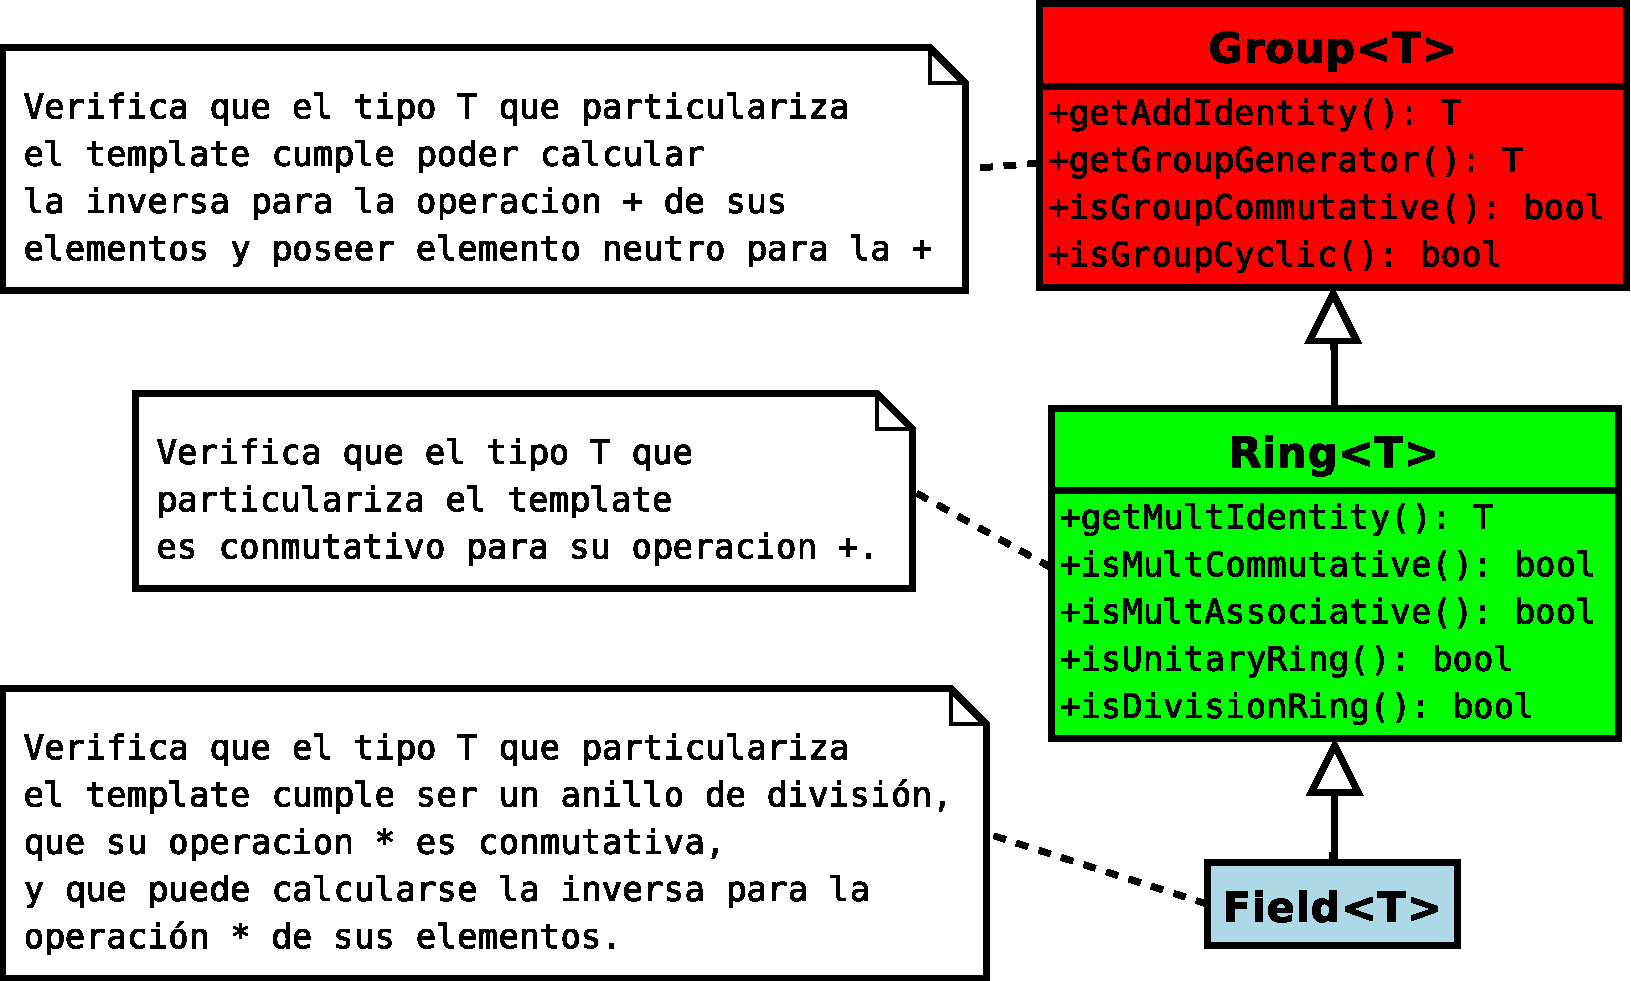
\includegraphics[width=0.95\textwidth,keepaspectratio]{categoriasAlgebraicas} 
    \caption{Categorias algebraicas}\label{fig:categoriasAlgebraicas}
  \end{figure}
  Cuando un tipo de dato de la librar�a (es decir, un hijo de \texttt{MPPDataType}) se
  encasilla dentro de esta jerarqu�a, sobre dicho tipo (representado mediante el par�metro 
  de plantilla \texttt{T}) se realizan una serie de comprobaciones, dise�adas para verificar
  que efectivamente dicho tipo cumple las condiciones impuestas por la categor�a 
  algebraica a la que aspira pertenecer. Esta serie de comprobaciones se realizan por medio
  de \emph{asertos}.



\begin{lstlisting}[captionpos=b,basicstyle=\footnotesize,frame=shadowbox,rulesepcolor=\color{black},language=C++,numbers=left,caption=STATIC\_ASSERT, label=lst:staticassert]
~Group() {
  STATIC_ASSERT( ValidateRequirements() );
}
(...)
static bool ValidateRequirements() {
  T (T::*getAddInverse)() const __attribute__ ((__unused__))  = &(T::getAddInverse) ;
  const T& (*getAddIdentity)() __attribute__ ((__unused__))  = &(T::getAddIdentity) ;
  const T& (*getGroupGenerator)() __attribute__ ((__unused__)) = &(T::getGroupGenerator) ;

  return true;
}
\end{lstlisting}


  \begin{figure}[h]
    \centering
    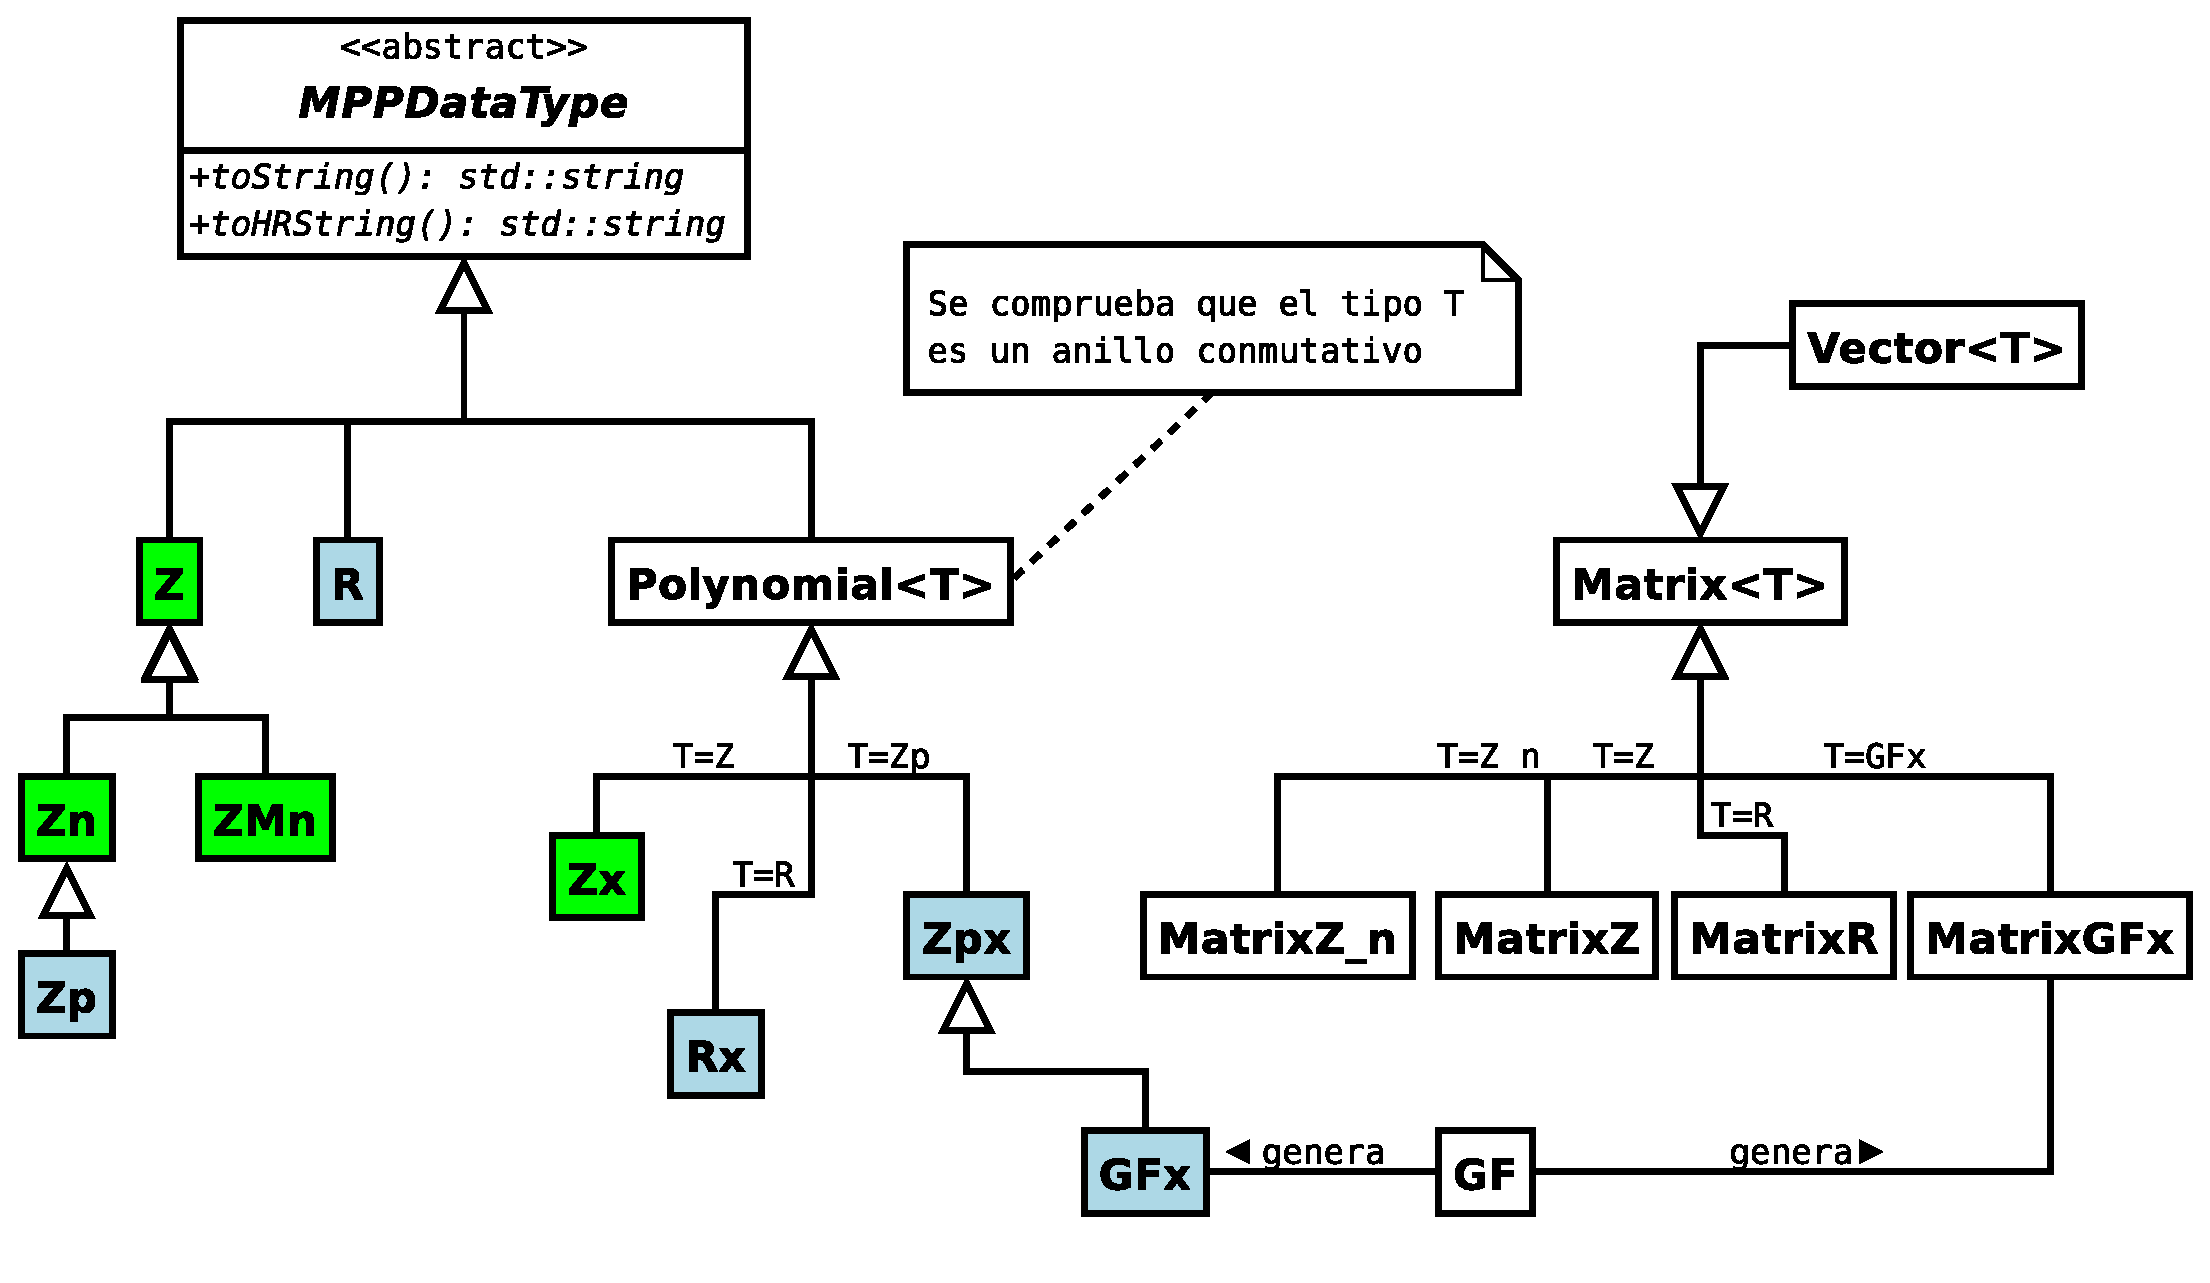
\includegraphics[width=0.95\textwidth,keepaspectratio]{categorizacionAlgebraica} 
    \caption{Categorizaci�n algebraica}\label{fig:categorizacionAlgebraica}
  \end{figure}




  \subsection{Enteros $\mathbb{Z}M_n$}\label{implZM_n}

  \subsection{Polinomios}\index{implementaci�n!polinomios}\label{impl:polinomios}
    totalmente genericos
  \subsubsection{Verificando el car�cter de $S$}
    tiene que ser como ser como minimo anillo conmutativo con unidad. Verificaciones estaticas
  \subsubsection{Operaciones dependientes de $S$}
    p ej, div en udf o  no, idem pa gcd  


  \subsection{Matrices}\index{tipos!Matrices}

\chapter{Paralelismo en la biblioteca}

\begin{flushright}
  \begin{minipage}[t]{13cm}
    \begin{flushright}
      \begin{quote}
        \emph{
          Right now I'm having amnesia and d�j� vu at the same time.
        }
        \begin{flushright}
          \textbf{\textemdash Stephen Wright (en paralelo).}
        \end{flushright}
      \end{quote}
    \end{flushright}
  \end{minipage}
\end{flushright}

\bigskip

\begin{center}{\line(1,0){325}}\end{center}

%--------------------------------------------------------%

\section{Introducci�n}

  Se ha hecho �nfasis en la paralelizaci�n de los m�todos b�sicos sobre los 
  que la mayor�a de las rutinas de m�s alto nivel se apoyan. Por varios motivos:
  \begin{description}
    \item[Por su propia naturaleza.] Como m�todos \emph{b�sicos}, son utilizados con 
    mucha mayor frecuencia, y por un abanico mayor de clientes. Cualquier optimizaci�n
    --en este caso la paralelizaci�n-- tendr� un efecto beneficioso directamente proporcional 
    dichos factores.
    \item[Facilidad.] La complejidad de los m�todos suele ser mayor en m�todos de m�s alto nivel.
    Por ejemplo, comp�rese la complejidad de los m�todos de factorizaci�n de enteros con la implementaci�n
    b�sica del producto de enteros. Es incluso probable que la adaptaci�n paralela de los actuales 
    m�todos secuenciales no sea posible sin una reescritura completa del m�todo. N�tese sin embargo como,
    en base al punto anterior, incluso los complejos m�todos no paralelizables s� se benefician de la paralelizaci�n
    de los b�sicos: siguiendo con el ejemplo de la factorizaci�n y el producto de enteros, el primer m�todo s� se valdr�
    del segundo y ser� \emph{parcialmente} paralelo de forma indirecta.
    \item[Modularidad.] Un m�todo b�sico es susceptible de ser reutilizado en alg�n otro lugar, haciendo gala de su
    modularidad. Consigo arrastrar� su condici�n de paralelo, haciendo extensiva esta caracter�stica incluso all� 
    donde no se ha hecho un esfuerzo expl�cito en este sentido. 
  \end{description}




  \subsubsection{Especificaci�n del paralelismo}
    Desgraciadamente, no existe una sintaxis universalmente aceptada para la especificaci�n
    de algoritmos paralelos. No ser� en esta memoria donde se contribuya a empeorar a�n m�s esta
    situaci�n, sino que nos ce�iremos a la sintaxis del la tecnolog�a utilizada para la obtenci�n
    de paralelismo en nuestros m�todos, OpenMP. Esto conlleva que el lector habr� de estar al menos
    parcialmente familiarizado con la sintaxis de este interfaz. Afortunadamente, no se trata de una
    familia de m�todos bastante reducida y de f�cil interpretaci�n. Para una introducci�n de apenas
    veinte p�ginas --pero ya suficiente para la comprensi�n del c�digo aqu� incluido--, v�ase 
    el ap�ndice A de \cite{parpatterns}. En cualquier caso, en la opini�n del autor, la mayor�a de 
    los ejemplos de c�digo son autoexplicativos aun utilizando las directivas de OpenMP.







\section{Potenciaci�n modular}
  \subsection{Dos hilos y $\mathbb{Z}M_n$}
  \cite{modexpmont}
  \subsection{Mi m�todo}

\section{Vectores}
  \subsection{Producto escalar}

\section{Matrices}
  \subsection{Producto}
  \subsection{Descomposici�n $LU$}
  \subsection{Inversi�n}
  \subsection{Transposici�n}
  \subsection{Determinante}
    \subsubsection{Algoritmo de Gauss-Bareiss}\label{para:bareiss}
    Descrito en la secci�n \ref{impl:bareiss}. Si se representa el patr�n de accesos derivado 
    de su algoritmo secuencial (algoritmo \ref{alg:bareiss}), no es dif�cil derivar una divisi�n
    en tareas basada en la secuencia de patrones de dise�o 
    (data decomposition/order tasks -> geom. decomposition -> loop paralelism)
    de \cite{parpatterns}. En la figura \ref{fig:accBar} 
    se muestra el patr�n de accesos para el algoritmo.  Los elementos de color verde
    indican accesos de \emph{lectura}, mientras que los de color rojo indican tambi�n \emph{escritura}.

   \begin{figure}[h]
    \centering
    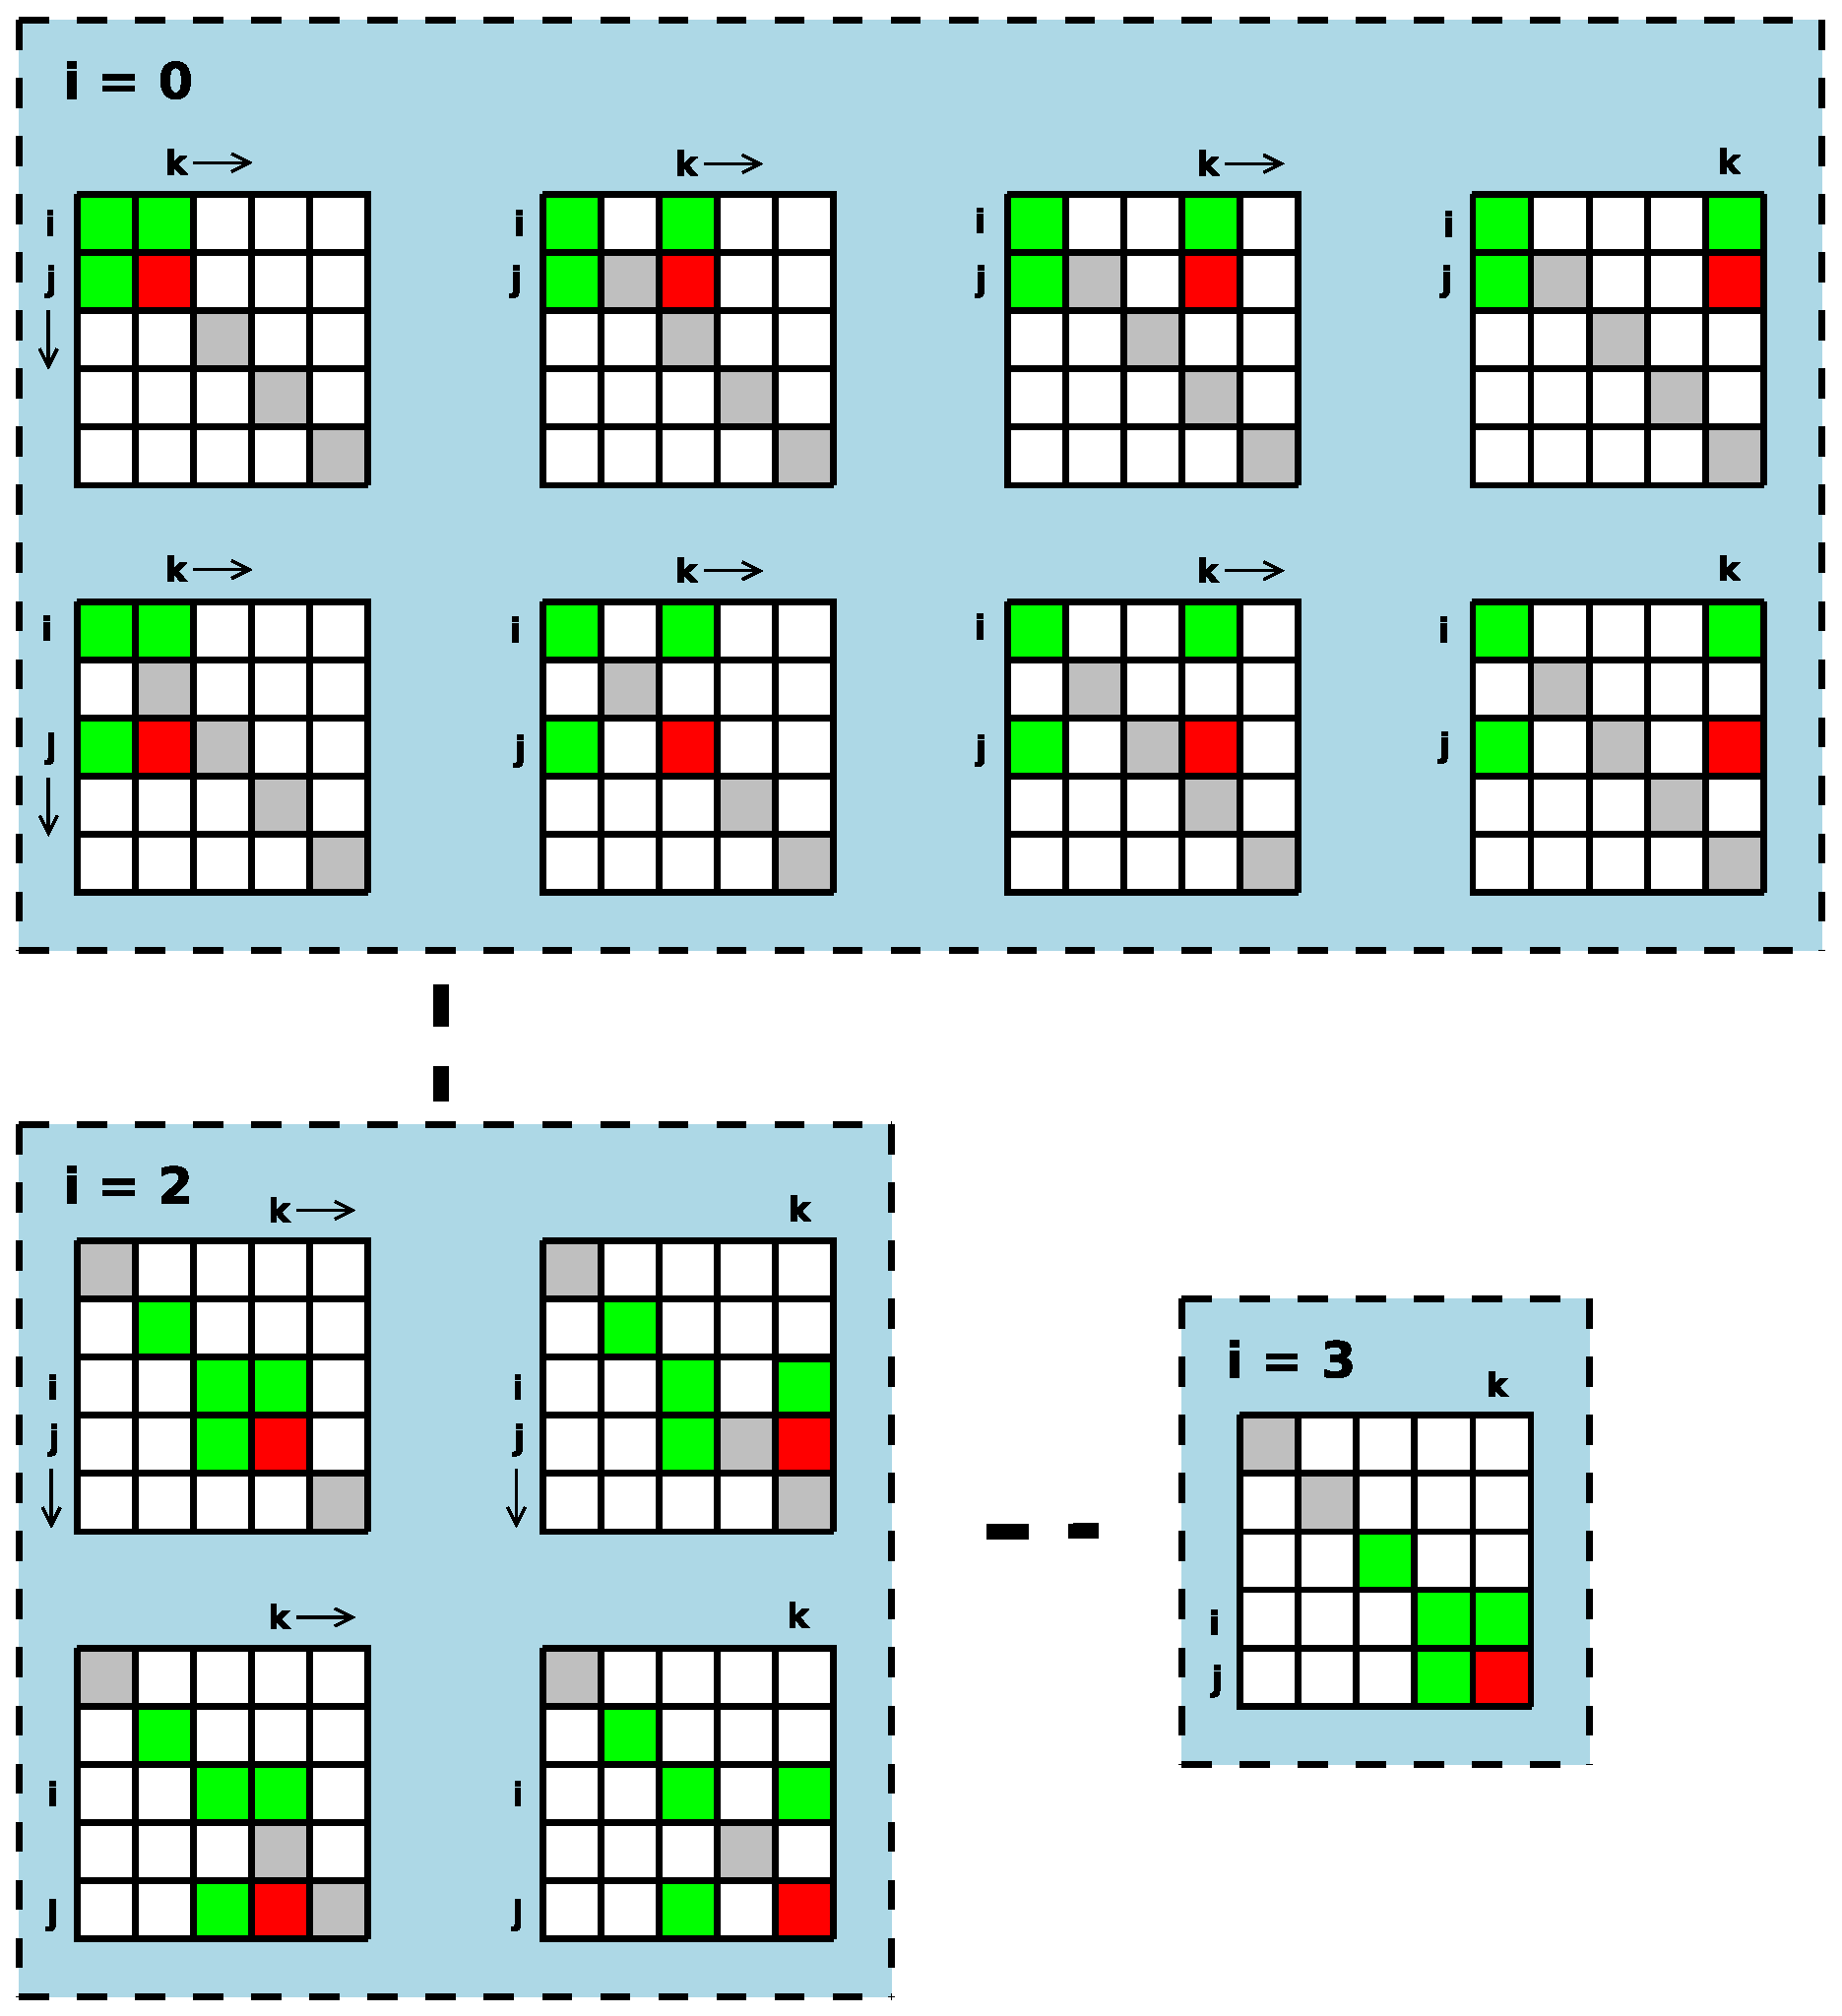
\includegraphics[width=0.95\textwidth,keepaspectratio]{patronAccesosBarreis} 
    \caption{Patr�n accesos Gauss-Bareiss}\label{fig:accBar}
  \end{figure}

  De este patr�n de acceso se deriva una paralelizaci�n organizada por el acceso a los datos y
  con una enumeraci�n lineal. Por tanto el patr�n estructural m�s indicado parece ser una descomposici�n
  geom�trica sobre las filas, siguiendo el recorrido de $k$. A nivel de estructura de soporte, el patr�n de 
  paralelismo de bucle se ajusta perfectamente: %FIXME

      \begin{algorithm}
        \caption{Algoritmo de Gauss-Bareiss}\label{alg:bareiss}
        \begin{algorithmic}[1]
          \Procedure{Gauss-Bareiss}{Matriz $M \in \mathcal{M}_{n \times n}$}
          \State $sign \gets 1$
          \For{$i \in \{0, \ldots, n-2\}$}
            \State $p \gets M_{i,i}$
            \If{$p = 0$}
              \If{$ \neg \mathrm{pivot(}$i$\mathrm{)} $} 
                \Statex \Comment{Si \textrm{pivot} es falso, no se ha podido pivotar}
                \State \textbf{Return} $0$ \Comment{Matriz singular}
              \EndIf
              \State $sign \gets -sign$ \Comment{Se ha permutado una fila}
              \State $p \gets M_{i,i}$ \Comment{$M_{i,i} \neq 0$}
            \EndIf
            \State \texttt{\#pragma omp parallel}
            \For{$j \in \{i+1,\ldots,n-1\}$}
              \State \texttt{\#pragma omp for}
              \For{$k \in \{i+1,\ldots,n-1\}$}
                \State $M_{j,k} \gets M_{j,k} * p - M_{j,i}*M_{i,k}$
                \If{ $i > 0$ }
                  \State $M_{j,k} \gets M_{j,k} / M_{i-1,i-1}$ \Comment{Esta divisi�n \emph{siempre} es exacta}
                \EndIf
              \EndFor %for k
            \EndFor %for j
          \EndFor %for i

          \State \textbf{Return } $sign * M_{n-1,n-1}$
          \EndProcedure
        \end{algorithmic}
      \end{algorithm}



  \subsection{Operaciones de car�cter vectorial}
    % sumas, restas, prod por escalares

\section{C�lculo de \textit{reducciones}}


\section{Polinomios}
  \subsection{Producto}
  \subsection{Operaciones de car�cter vectorial}
    % sumas, restas, prod por escalares
  \subsection{Evaluaci�n}\label{parallel:evalPoly}
    \cite{dorn}



\include{resultados}
%% CAPITULO SOBRE FUNCIONES TRASCENDENTES

\chapter{Funciones trascendentes}\label{cap:primos}

\begin{flushright}
  \begin{minipage}[t]{13cm}
    \begin{flushright}
      \begin{quote}
        \emph{
         cita
        }
        \begin{flushright}
          \textbf{\textemdash D. Zagier}
        \end{flushright}
      \end{quote}
    \end{flushright}
  \end{minipage}
\end{flushright}

\bigskip

\begin{flushright}
  \begin{minipage}[t]{13cm}
    \begin{flushright}
      \begin{quote}
        \emph{
        cita 2
        }
        \begin{flushright}
          \textbf{\textemdash H. Montgomery}
        \end{flushright}
      \end{quote}
    \end{flushright}
  \end{minipage}
\end{flushright}

\bigskip

\begin{center}{\line(1,0){325}}\end{center}

%--------------------------------------------------------%

\section{Introducci�n}
\section{La funci�n exponencial}
  
  \subsection{Exponencial inversa: la funci�n logaritmo}
    \begin{observacion}\label{obsLog}
      Si $x \in \mathbb{R}$, existe un $n \in \mathbb{N}$ tal que
      $2^{n-1} < x \leq 2^n$. Entonces, si $y = x/2^n$, se verifica
      que $0 < y \leq 1$
    \end{observacion}

    En base a la observaci�n \ref{obsLog}, el c�lculo de $x \in
    \mathbb{R}$ se reducir�a a (utilizando los s�mbolos de dicha
    observaci�n):
    \[
      \log{(x)} = \log{(y \times 2^n)} = \log{(y)} + n \cdot \log{(2)}
    \]
    Las ventajas que de esta forma de calcula el logaritmo se
    desprenden son claras: por una parte, el c�lculo de $\log(2)$ (tambi�n denominada
    ``La constante logar�tmica'', v�ase \cite{log2}) es un problema
    ampliamente tratado y existen m�todos de gran eficiencia para su c�lculo. 
    M�s adelante se tratar� este punto en m�s profundidad.
    Por otra parte, al cumplirse $0 < y \leq 1$, el c�lculo de
    $\log{(y)}$ puede realizarse satisfactoriamente y con relativa
    efectividad utilizando la expansi�n de MacLaurin
    para la funci�n logaritmo.

    \subsubsection{La constante logar�tmica}

    


  
\section{Funciones trigonom�tricas}

  \subsection{El c�lculo de las inversas}



% CAPITULO SOBRE EL SERVIDOR XMLRPC Y EL CLIENTE EN PYTHON

\chapter{MPPLab: (una) ventana a la biblioteca}

\begin{flushright}
  \begin{minipage}[t]{13cm}
    \begin{flushright}
      \begin{quote}
        \emph{
        }
        \begin{flushright}
          \textbf{\textemdash .}
        \end{flushright}
      \end{quote}
    \end{flushright}
  \end{minipage}
\end{flushright}

\begin{center}{\line(1,0){325}}\end{center}

%--------------------------------------------------------%


\section{Motivaci�n}
  Una biblioteca como la que es el eje principal de este trabajo no es
  algo f�cil de apreciar a primera vista. Puede que, y ojala as� sea,
  quien se aventurase en la lectura de su c�digo o concediese el beneficio
  de la duda tras la lectura de la presente memoria, pudiera hacerse una
  idea -para bien o para mal- de su valor. Sin embargo, no se pretende poner
  un peso tal en el lector. Es m�s bien nuestra responsabilidad e intenci�n el
  mostrarle al menos parte de su potencial, de una forma tanto atractiva
  como vers�til y �til. Asimismo, sirve para poner en pr�ctica destrezas y
  t�cnicas que no son f�cilmente aplicables al desarrollo de una
  biblioteca.

  En t�rminos m�s concretos, se buscaba el proporcionar una manera de
  interactuar con los m�todos ofrecidos por la biblioteca sin necesidad de
  bajar al nivel del c�digo. Si bien para una explotaci�n exhaustiva de todos
  los mecanismos de la misma se hace necesario utilizarla realmente como
  una biblioteca -esto es, programando-, no es �bice para exponer aquellos
  que, aunque s�lo en parte, muestren qu� se ha desarrollado.

  Con este fin, e inspirados en conocidos paquetes para el trabajo en
  Matem�ticas, tales como MatLab o Mathematica, se opt� por un interfaz
  gr�fico pero guiado por instrucciones textuales. Es m�s, las
  sentencias aceptadas por el cliente que se describe en el punto \ref{cliente}
  son un superconjunto del popular lenguaje de \textit{scripting}
  Python\footnote{\url{http://www.python.org}}. �Por qu� se habla de
  �cliente�? Porque el dise�o adoptado ha sido una arquitectura
  cliente/servidor como se expone a continuaci�n. Esto aporta una serie de
  beneficios nada despreciables y brinda una vez m�s la oportunidad de
  ampliar el espectro de campos t�cnicos cubiertos en el presente trabajo.


\section{Desarrollo}
  
  \subsection{Arquitectura}\label{arquitectura}
  La especificaci�n de una arquitectura depende siempre de los requisitos del sistema 
  a modelar. En el caso que nos ocupa, los requisitos pueden resumirse en:
  \begin{itemize}
    \item Posibilidad de ejecuci�n de m�ltiples clientes de forma simult�nea.
    \item Independencia entre clientes: cada cliente debe poder considerar ser el �nico
    utilizando el servidor (exceptuando cuestiones de rendimiento y/o perfilado).
  \end{itemize}

  En la figura \ref{fig:archClienteServidor} se representa el esquema adoptado.

  \begin{figure}[h]
    \centering
    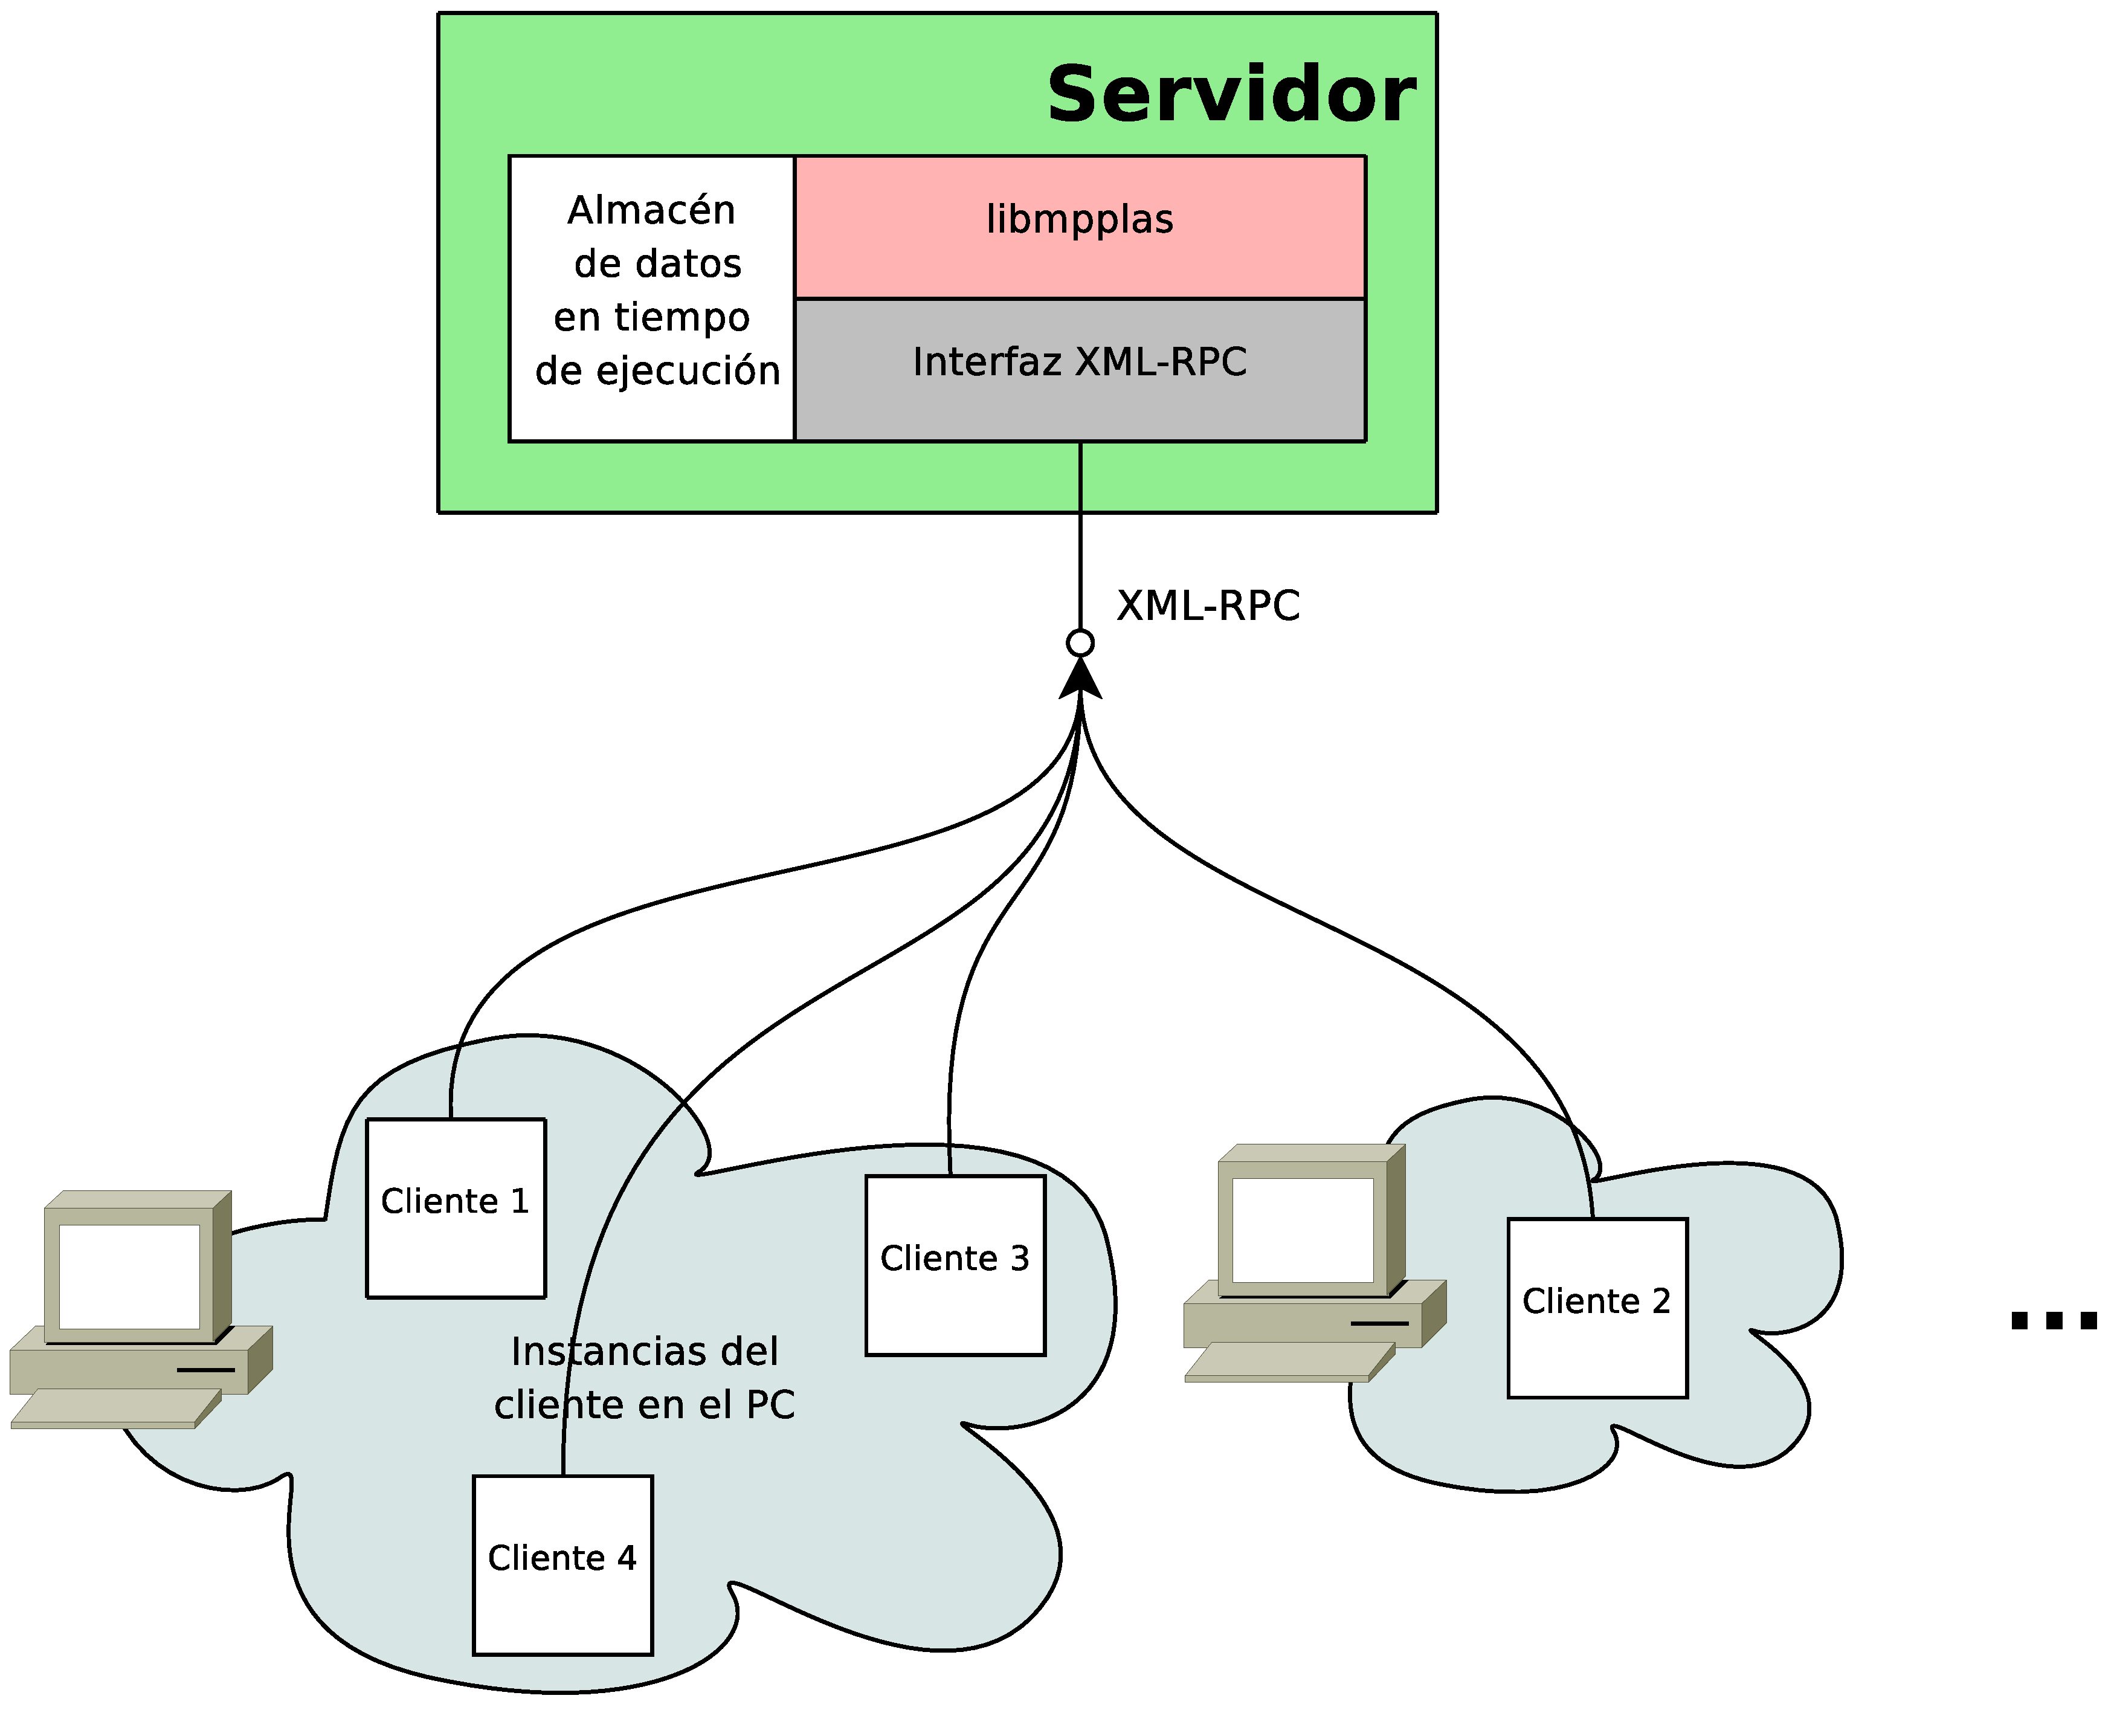
\includegraphics[width=0.95\textwidth,keepaspectratio]{ClientServerArch} 
    \caption{Esquema de la arquitectura cliente/servidor}\label{fig:archClienteServidor}
  \end{figure}

  Como puede verse en dicha figura, se ha optado por utilizar el protocolo
  XML-RPC (\cite{xmlrpcspec}), por tratarse de un protocolo perfectamente
  indicado para la tarea a desempe�ar: existen implementaciones del mismo en 
  pr�cticamente todos los lenguajes de programaci�n mayoritarios, es sencillo aunque
  tambi�n potente, y muy versatil. Incluso, dado que descansa sobre el protocolo 
  HTTP, es posible el cifrado y/o compresi�n de los datos que maneja. 

  La capa que implementa los servicios XML-RPC se comunica directamente con los m�todos
  de la biblioteca desarrollada, y ambas recurren a un almac�n de datos en tiempo de ejecuci�n
  para el intercambio de informaci�n (v�ase secci�n \ref{par:runtimeData}).


  \subsection{El servidor}
    Abarca la implementaci�n de una capa cuya funci�n es esperar a recibir peticiones
    XML-RPC de m�todos exportados al cliente para posteriormente adaptarlas a las llamadas
    correspondientes a m�todos de la biblioteca MPPLAS. Gestiona tambi�n todas las instancias
    de los datos creados en cada uno de los clientes. Estos puntos se desarrollan en mayor
    profundidad en las siguientes secciones.

    \paragraph{Caracter�sticas}
      \begin{itemize}
        \item Exporta m�todos mediante XML-RPC (basado en la biblioteca \texttt{xmlrpc-c}
            \footnote{\url{http://xmlrpc-c.sourceforge.net/}}
        \item Multihilo (basado en \texttt{pthreads})
        \item Gesti�n din�mica de datos de los clientes en tiempo de ejecuci�n
        \item Mecanismos de recogida de basura (\textit{Garbage Collection})
      \end{itemize}


      \subsubsection{Utilizaci�n de XML-RPC}
        Por las razones expuestas anteriormente (v�ase \ref{arquitectura}), el servidor 
        pone a disposici�n de los clientes una serie de m�todos mediante el protocolo 
        XML-RPC. Otra ventaja adicional del uso de esta tecnolog�a son las capacidades de
        \emph{introspecci�n} que ofrece\footnote{esto ser� de suma relevancia para la implementaci�n
        del cliente, v�ase la secci�n \ref{boostrapping}}. Es decir, el propio servidor
        es capaz de dar informaci�n sobre qu� m�todos ofrece. El hecho de que el protocolo
        HTTP, sobre el que XML-RPC descansa, est� orientado a transacciones (v�ase \cite{stallings},
          pp. 676 y siguientes, para una descripci�n de este protocolo), siendo estas \emph{independientes}
        y no guardando ninguna informaci�n de estado en ellas, posibilita una gesti�n de errores m�s sencilla.
        Por ejemplo, si la comunicaci�n entre cliente y servidor se ve interrumpida temporalmente, no es
        necesario reestablecer ninguna conexi�n posteriormente, ya que cada una de las operaciones a
        nivel cliente-servidor es independiente de las dem�s.

      \subsubsection{Multihilo}
        Si se pretende soportar que varios clientes puedan operar de forma concurrente e 
        independiente, es necesario soportar de alguna forma la ejecuci�n multihilo. 
        El protocolo XML-RPC descansa sobre el conocido HTTP, con lo que un servidor 
        XML-RPC no es m�s que un servidor HTTP ampliado: toda la gesti�n del tr�fico 
        subyacente se realiza mediante este segundo protocolo. La ventaja que esto aporta
        es la existencia de numerosas soluciones para la implementaci�n de un servidor
        HTTP, entre ellas las soluciones multihilo. Para este trabajo se ha utilizado
        el servidor HTTP incluido con la biblioteca \texttt{xmlrpc-c}, el cual incorpora
        soporte multihilo basado en la biblioteca \textit{pthreads}.

        Por tanto, y sin necesidad de implementar nada por nuestra parte, nuestro servidor
        manejar� peticiones XML-RPC desde los clientes de forma simult�nea e independiente.

  \subsubsection{Gesti�n din�mica de datos de los clientes en tiempo de ejecuci�n.}\ref{par:runtimeData}
    En el transcurso de una sesi�n de utilizaci�n del ciente, indudablemente se crear�n
    instancias de los diferentes tipos de datos disponibles. Instancias que se corresponden,
    en el fondo, con datos de la biblioteca. Es necesario por tanto disponer de un mecanismo
    de almacenaje y recuperaci�n eficaz y eficiente que permita trabajar comodamente con
    los datos que el usuario vaya creando. Asimismo, habr� de cumplir tambi�n otros 
    requisitos impuestos por el cliente y la biblioteca, como son el ser \textit{thread-safe}
    y gestionar multiplies clientes de forma simult�nea.

    \begin{figure}[h]
      \centering
      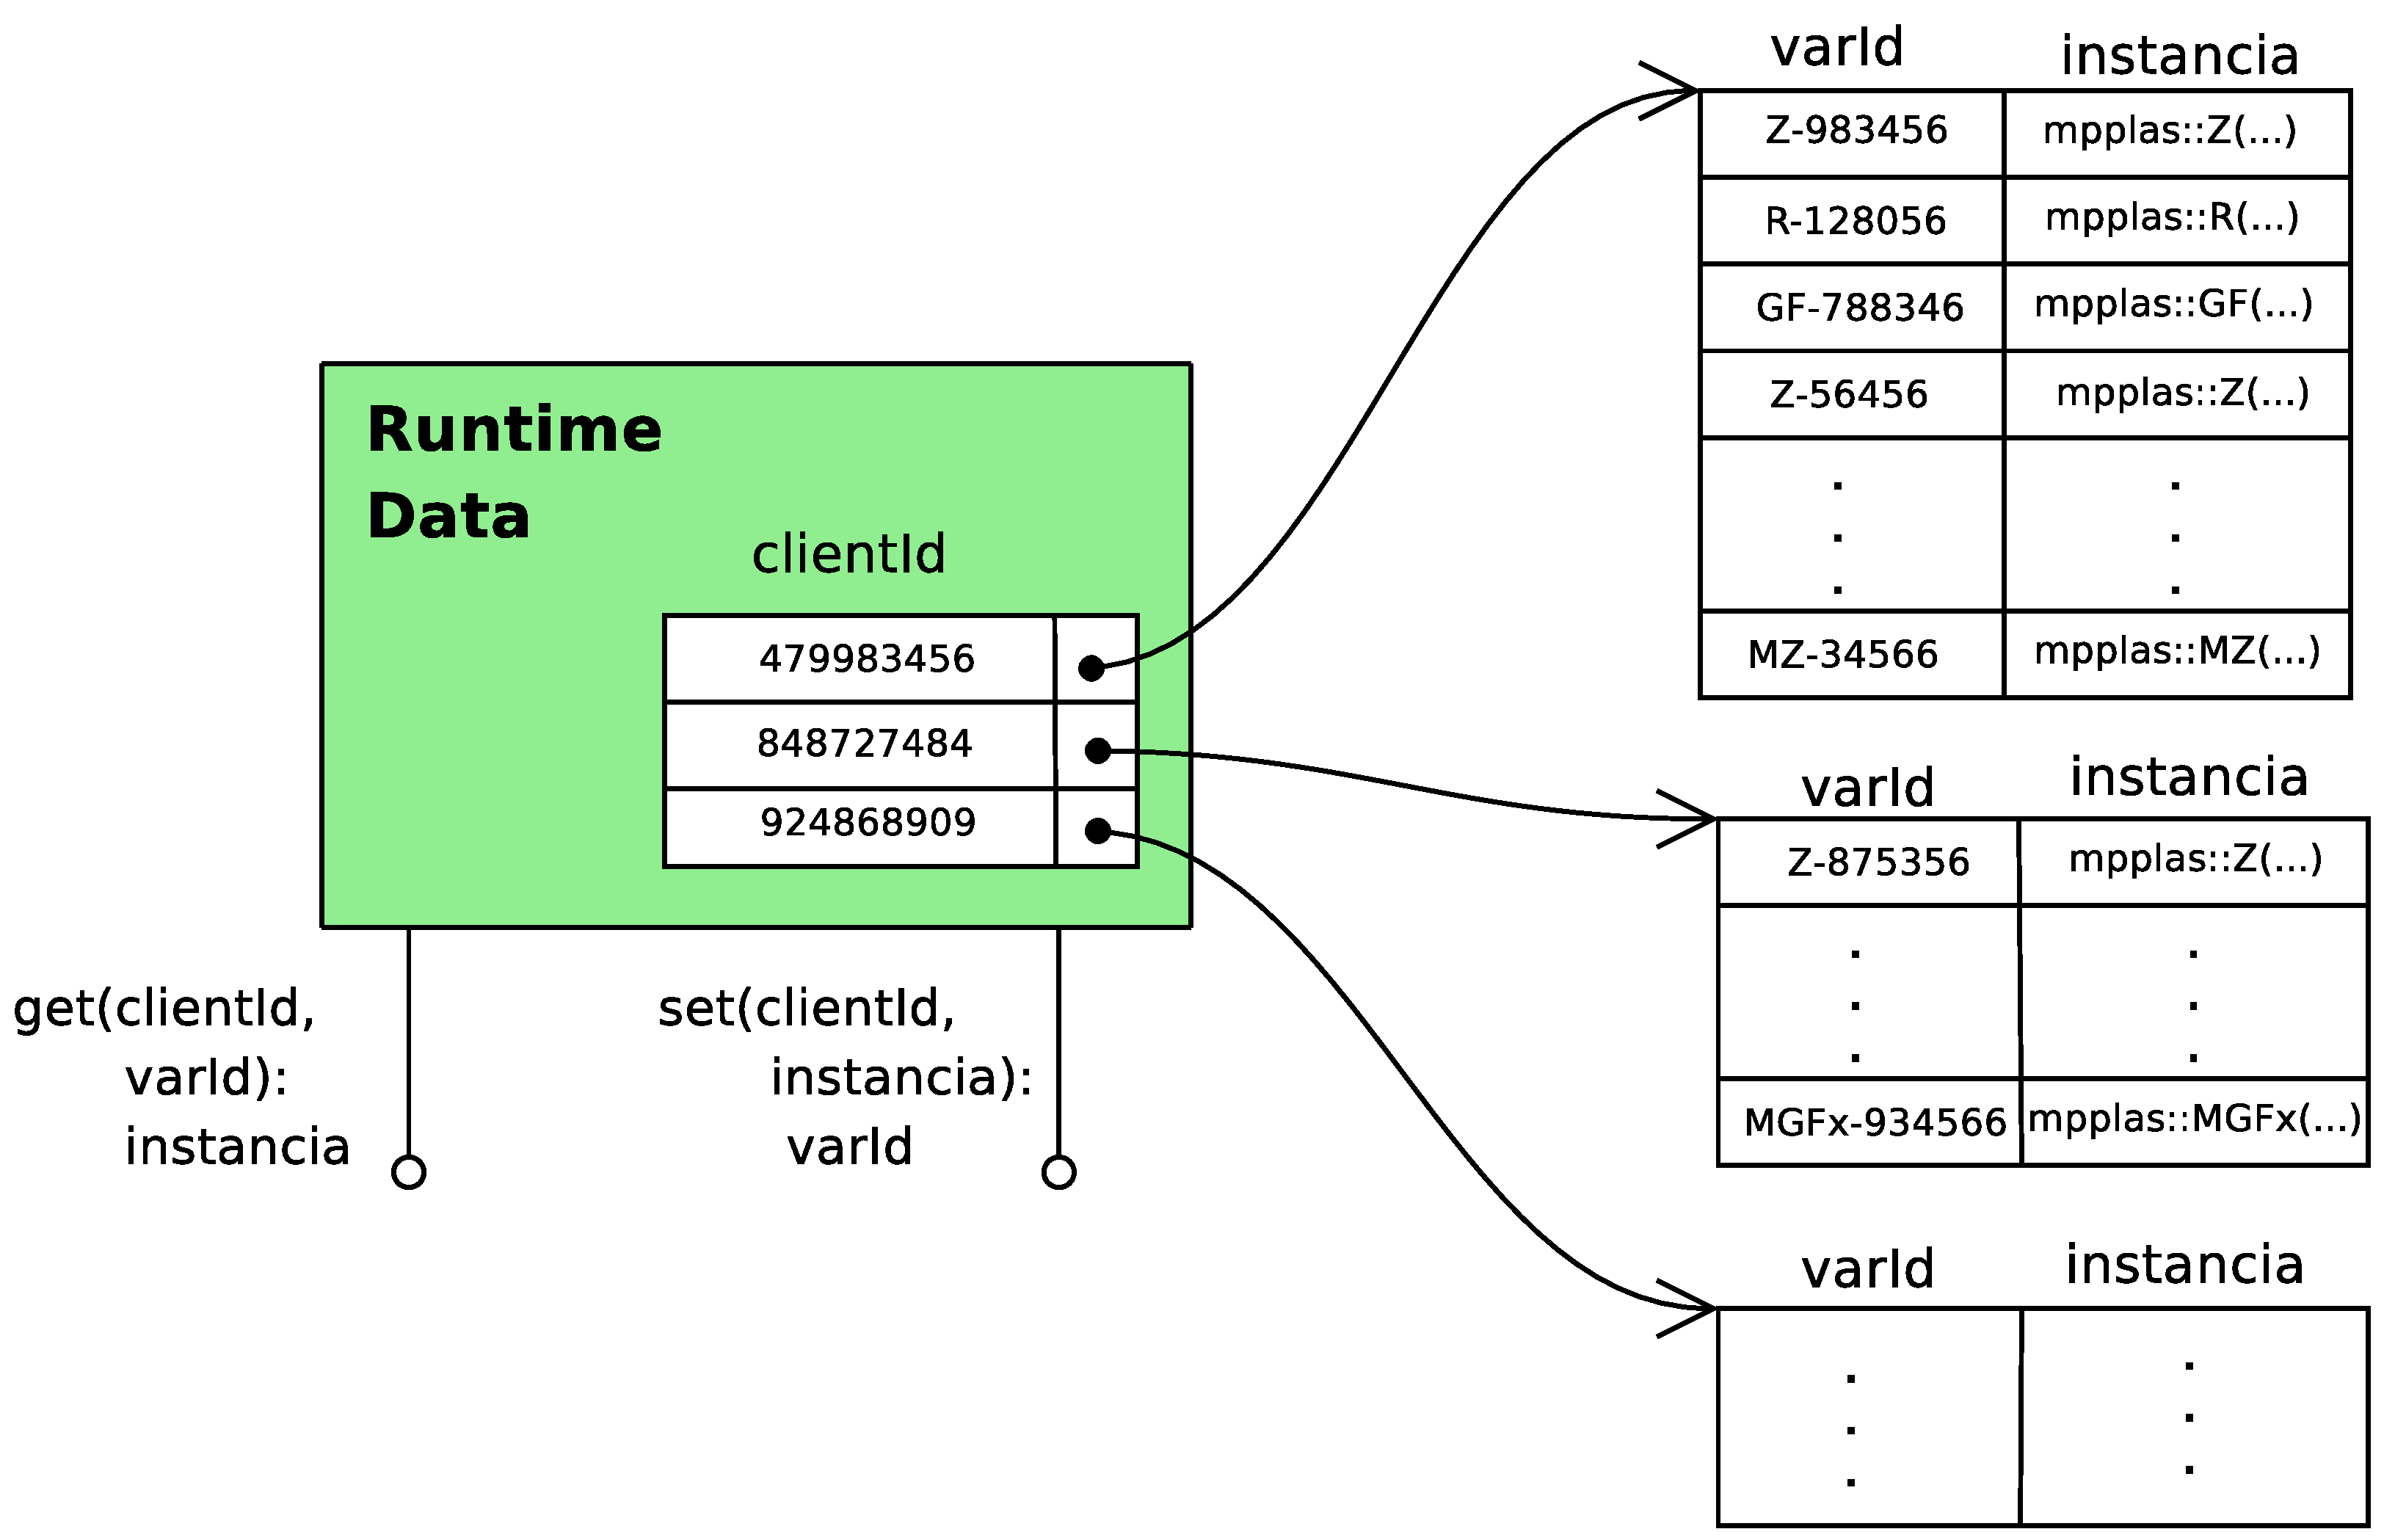
\includegraphics[width=0.95\textwidth,keepaspectratio]{runtimeData} 
      \caption{Esquema de la arquitectura cliente/servidor}\label{fig:runtimeData}
    \end{figure}

    El mecanismo implementado se representa en la figura \ref{fig:runtimeData}. En �sta
    se representa a \textit{grosso modo} el modo de funcionamiento de este almac�n 
    de datos din�micos: a cada cliente conectado al servidor se le asigna un identificador
    de cliente (\texttt{clientId}) �nico. Mediante este identificador, se posibilita a 
    los clientes a insertar y recuperar sus datos. El almacen de datos asigna un identificador
    de variable (\texttt{varId}) �nico (por cliente) tras cada inserci�n de un nuevo dato. 
    Es mediante este identicador de variable que el cliente puede posteriormente recuperar 
    el dato de forma un�voca.

    Todas las operaciones est�n, como se indicaba anteriormente, preparadas para soportar 
    la ejecuci�n sobre m�ltiples hilos. Para esto, se utilizan rutinas de la biblioteca \textit{pthreads},
    ya que es este sistema mediante el que el servidor soporta la ejecuci�n concurrente de varias
    peticiones. Por ejemplo:

\lstset{escapeinside={(*@}{@*)}}
\begin{lstlisting}[captionpos=b,basicstyle=\footnotesize,frame=shadowbox,rulesepcolor=\color{black},language=C++,numbers=left,
  caption=Ejemplo de protecci�n de secci�n cr�tica con pthreads]
  template<typename T>
  varId_t RuntimeData<T>::set(const clientId_t clientId, 
      const T& instance, 
      const std::string typeStr){
    pthread_mutex_lock( &_mutex ); (*@\label{alg:acquire}@*)
    const varId_t varId( _getAvailableVarId(clientId, typeStr) );
    _dataTable[clientId][varId] = instance;
    pthread_mutex_unlock( &_mutex ); (*@\label{alg:release}@*)
    return varId;
  }
\end{lstlisting}

  En la l�nea \ref{alg:acquire}, se asegura la secci�n cr�tica con un  \textit{lock} de \textit{pthreads}, que se libera
  al final de la misma, en la l�nea \ref{alg:release}.


    \subsubsection{Recogida de basura.} Se ha descrito c�mo los datos, las instancias,
    son almacenadas en el servidor. Sin embargo, �cu�ndo se destruyen?
    Cada vez que se tiene un resultado de un c�lculo, incluso temporales
    como la suma en una expresi�n del tipo $3*(4+5)$, una nueva
    instancia del tipo adecuado es creada y almacenada. Adem�s, nada 
    impide al cliente dejar que el resultado se pierda: no es necesario 
    asignar siempre un resultado a una variable. 
    
    D�ndole la vuelta a la cuesti�n: �qu� \emph{s�} debe conservarse,al
    menos hasta la desconexi�n del cliente? Aquellas instancias
    asociadas a una variable. Es decir, no debe darse el caso de una
    variable cuyos datos, los datos a los que apunta, no existan. Dado
    que la gesti�n de las variables corre a cuenta del cliente, el
    servidor recibe tan solo una lista de los identificadores de
    variables a conservar. El resto de identificadores y sus instancias
    asociadas ser�n eliminados y los recursos que utilizasen,
    liberados. Esto se corresponde con una de las formas m�s sencillas
    de recolecci�n de basura, (A COMPLETAR CON LAS REFERENCIAS).
    Afortunadamente, cubre nuestras necesidades satisfactoriamente. 

    El campo de los recolectores de basura es amplio y complejo, y su
    bibliograf�a abundante. Posiblemente los entornos de ejecuci�n m�s
    popular que utiliza esta t�cnica son las diferentes implementaciones 
    del \textit{Java Runtime Environment}. 
    En el momento de redactar estas l�neas, la inclusi�n de recolectores
    de basura est� incluida dentro del borrador de la nueva revisi�n del
    lenguaje C++,
    C++0x\footnote{\url{http://www.open-std.org/jtc1/sc22/wg21/}}
      

  \subsection{\emph{Un} cliente}\label{cliente}
    El �nfasis en el art�culo indeterminado �un� en el t�tulo no es
    casual: dada la versatilidad del protocolo XML-RPC, servidor y
    cliente est�n completamente desacoplados. Por tanto, la presente
    implementaci�n es tan solo una de las posibles que podr�an
    utilizarse para �dialogar� con el servidor. De hecho, como apoyo a 
    estas afirmaciones, se describe en el punto \ref{otroCliente} una
    peque�a -su objetivo es tan solo ilustrar este punto- implementaci�n
    de un cliente alternativo realizada en JavaScript.

    \paragraph{Caracter�sticas}
      \begin{itemize}
        \item \textit{Bootstrapping}: inspecci�n de m�todos disponibles
              en el servidor, realizando \emph{el propio cliente} la
              escritura e interpretaci�n del c�digo necesario para su 
              utilizaci�n
        \item F�cilmente configurable
        \item Soporte para \textit{plotting}
        \item Multiplataforma
        \item Actualizaciones autom�ticas
        \item Multihilo, pudiendo de ser explotado expl�citamente por el usuario.
        \item Basado en el lenguaje Python: ofrece todas las
        funcionalidades de este lenguaje.
      \end{itemize}

    \subsubsection{\textit{Bootstrapping} y autoescritura.}\label{boostrapping}
      Una de las caracter�sticas m�s destacables de este cliente es su habilidad para
      �escribirse a s� mismo�. Esto es posible debido fundamentalmente a dos razones:
      la capacidad de Python de interpretar c�digo en tiempo de ejecuci�n y los mecanismos
      de introspecci�n que el servidor XML-RPC ofrece.

      �A qu� nos estamos refiriendo cuando hablamos de �autoescritura�? A la capacidad
      de incorporar en el cliente m�todos ofrecidos por el servidor de forma autom�tica en tiempo
      de ejecuci�n, y por tanto sin necesidad de modificar el cliente. 

      %TODO

    \subsubsection{F�cilmente configurable.}
    \subsubsection{\textit{Plotting}.}
    \subsubsection{Actualizaci�n autom�tica.}
    \subsubsection{Multihilo.}


    El resto de las caracter�sticas, ser multiplataforma y un
    superconjunto de Python, derivan de la base utilizada: la
    biblioteca WxPython\footnote{\url{http://www.wxpython.org/}}.
    %TODO: completar un poco m�s.
    Las ventajas de utilizar Python como base son numerosas. Podr�a 
    parecer que complicase la utilizaci�n del cliente, por
    tener que lidiar con este lenguaje; por contra, la sencilla e
    intuitiva sintaxis del mismo minimiza este efecto. De haber
    implementado lenguaje propio para el cliente, su sintaxis no habr�a 
    podido ser mucho m�s simple, y casi con toda seguridad mucho menos
    potente. 



  \subsubsection{Muestra de cliente alternativo}\label{otroCliente}
    Utilizar el protocolo XML-RPC por parte del servidor a la hora de exportar 
    servicios resulta en una gran flexibilidad. Tanto es as� que con
    un m�nimo de codificaci�n se ha implementado un prototipo (ya que
    s�lo es una muestra de concepto, carece de grandes
    sofisticaciones) en JavaScript, lo que posibilita el acceso a los
    m�todos del servidor desde cualquier navegador con int�rprete de
    este lenguaje.
    %TODO

  \subsection{Peque�o manual de utilizaci�n}
      \paragraph{Consideraciones generales}
      Ciertos aspectos pueden chocar al primera vista, o ser considerados como errores, aunque en ocasiones
      su uso pueda resultar ventajoso. Sirva de ejemplo, la copia de variables:
      Tal como se ha expuesto en \ref{arquitectura}, el cliente trabaja con \emph{referencias} a las instancias
      de los datos almacenados en el servidor. Cuando en el interfaz Python del cliente, se ejecuta una asignaci�n
      \texttt{var1 = var2}, lo que se asigna a \texttt{var1} en realidad es tal referencia, con lo cual \texttt{var1}
      y \texttt{var2} har�an referencia a la misma variable. Cualquier modificaci�n \textit{in situ} del dato 
      apuntado ser�a visible a trav�s tanto de \texttt{var1} como de \texttt{var2}.

      �C�mo evitar este comportamiento? Es habitual, y necesario en muchas ocasiones, el querer realizar 
      copias \emph{independientes} de los datos. El modo de lograrlo es invocando \emph{el constructor} del tipo
      a copiar. Por ejemplo:

\begin{verbatim}
>>> var1 = MZ("[1 2; 3 4]")
>>> print var1
[  1  2 ]
[  3  4 ]

>>> var2 = var1
>>> print var2
[  1  2 ]
[  3  4 ]

>>> var1[(1,0)] = Z(321)
>>> print var1
[    1  2 ]
[  321  4 ]

>>> print var2
[    1  2 ]
[  321  4 ]

>>> var3 = MZ(var1)
>>> print var3
[    1  2 ]
[  321  4 ]

>>> var1[(1,0)] = Z(456)
>>> print var1
[    1  2 ]
[  456  4 ]

>>> print var3
[    1  2 ]
[  321  4 ]
\end{verbatim}

      En el ejemplo anterior, \texttt{var3} es creada mediante una llamada al constructor \texttt{MZ}, con lo que
      se crea una \emph{nueva instancia} de una matriz sobre los enteros, inicializada con los valores de \texttt{var1}.

    \subsubsection{Tipos disponibles}
       \paragraph{Z} Representa un entero de precisi�n arbitraria. Para crear un tipo de dato de este tipo, basta con 
       invocar a su constructor de la siguiente manera: 
\begin{verbatim}
>>> unEntero = Z('35872687327373')
\end{verbatim}
        Las operaciones sobre enteros son las b�sicas:
\begin{verbatim}
>>> otroEntero = getRandomZ(100)
>>> print unEntero, otroEntero
35872687327373 621786157705605499575785094237
>>> unEntero + otroEntero
621786157705605535448472421610
>>> unEntero - otroEntero
-621786157705605463703097766864
>>> unEntero * otroEntero
22305140419861824038317960677452898474649401
>>> unEntero / otroEntero
0
>>> unEntero % otroEntero
35872687327373
>>> pow(unEntero, otroEntero, Z(11234)) #exponenciaci�n modular
1357
\end{verbatim}

       \paragraph{R} Representa un real de precisi�n arbitraria. Su utilizaci�n es muy similar al tipo de dato para 
       enteros, con la salvedad de poder controlar tanto el n�mero de bits utilizados para manejar su precisi�n interna
       como cuantos d�gitos en base $10$ son mostrados:
\begin{verbatim}
>>> unReal = R('1.78346873235353')
>>> R.setOutputPrecision(3)
>>> print unReal
1.783
>>> R.setInnerPrecision(2000)
>>> unReal = R('1.78346873235353')
>>> R.setOutputPrecision(0) #usar m�xima precisi�n
>>> print unReal
1.783468732353530000(...)000
\end{verbatim}
       \paragraph{GF} Representa un Cuerpo Finito, a modo de generador de elementos del mismo. 
       Es posible obtener informaci�n acerca del cuerpo mediante el m�todo \texttt{getProperties()}. Los elementos
       del cuerpo se obtienen mediante el m�todo \texttt{getElement()}.
       En el siguiente p�rrafo se incluyen ejemplos, junto con los correspondientes a \texttt{GFx}.

       \paragraph{GFx} Representa un elemento de un Cuerpo Finito.
       Al igual que en el caso anterior, y por comodidad, se puede obtener informaci�n acerca del cuerpo finito
       al que pertenece el elemento mediante el m�todo \texttt{getProperties()}. Asimismo, otros m�todos disponibles
       en este tipo de dato son: 
       \begin{description}
        \item[\texttt{getInverse()}] Devuelve la inversa del elemento sobre el que se aplica el m�todo.
        \item[\texttt{getPBRString()}] Devuelve una cadena de caracteres representado en polinomio correspondiente
        al elemento sobre el que se aplica.
        \item[\texttt{setValue(z)}] Asigna al elemento sobre el que se aplica el m�todo el valor del entero $z$ argumento
        dentro del cuerpo finito.
        \end{description}

        El siguiente ejemplo ilustra los puntos reci�n descritos:
\begin{verbatim}
>>> gf = GF(p=2, n=4, usePrimitive=True)
>>> gf.getProperties()
{'characteristic': '2', 'modulus': ' +1*x^4 +1*x^3 +1', 
  'isModulusPrimitive': True, 'order': '16', 'degree': 4}
>>> e = gf.getElement(123)
>>> print e
11
>>> print e.getPBRString()
 +1*x^3 +1*x^1 +1
>>> print e.getInverse()
10
>>> print e.getInverse() * e
1
>>> e.setValue(65)
[(1, 0)]
>>> print e
1
>>> print e.getInverse()
1
\end{verbatim}

       \paragraph{MZ} Representa una matriz sobre el anillo de los enteros. Existen ciertos aspectos comunes
       a los tipos matriciales, tales como el acceso a los elementos, la informaci�n sobre las dimensiones 
       y la transposici�n.
       Sin perdida de generalidad, v�ase el siguiente ejemplo para una matriz sobre los enteros:
\begin{verbatim}
>>> mat = MZ("[1231 47323213; -383485 124224]")
>>> print mat
[     1231  47323213 ]
[  -383485    124224 ]

>>> print mat[(0,0)]
1231
>>> mat[(0,0)] = Z('0')
>>> print mat
[        0  47323213 ]
[  -383485    124224 ]
>>> m = MZ("[ 1 2 3 ; 4 5 6 ; 7 8 9]")
>>> print m.getTranspose()
[  1  4  7 ]
[  2  5  8 ]
[  3  6  9 ]

>>> print m.getSubMatrix(rows=(2,), cols=(1,2))
[  8  9 ]

>>> print m.getSubMatrix(rows=(1,), cols=(1,2))
[  5  6 ]
[  8  9 ]

>>> print m.getSubMatrix(rows=(2,2), cols=(1,2))
[  8  9 ]

>>> print m.getSubMatrix(rows=(0,1), cols=(0,2))
[  1  2  3 ]
[  4  5  6 ]

>>> print m.getSubMatrix(cols=(0,2))
[  1  2  3 ]
[  4  5  6 ]
[  7  8  9 ]

>>> print m.getSubMatrix(cols=(0,1))
[  1  2 ]
[  4  5 ]
[  7  8 ]

>>> print m.getSubMatrix(cols=(0,0))
[  1 ]
[  4 ]
[  7 ]

>>> print m.getSubMatrix(cols=(2,1))
Traceback (most recent call last):
(...)
    raise Fault(**self._stack[0])
Fault: <Fault 0: 'Invalid Argument error: Invalid range; Invalid interval for submatrix operator (columns)'>
>>> 

\end{verbatim}

 La operaci�n de acceso a una submatriz opera de la siguiente manera:
  \begin{description}
    \item[\texttt{getSubMatrix(rows=(i,f), cols=(i,f))}] Devuelve la submatriz formada por 
    las filas/columnas especificadas por $i$ (de inicio) y $f$ (de fin). Ambas filas/columnas
    del interval son \emph{incluidas}. Si se omite el elemento $f$, como se aprecia en los ejemplos,
    se considerar�n a $f$ como la �ltima fila/columna. 
  \end{description}


       Tambi�n es posible crear una matriz especificando sus dimensiones. Ser� inicializada con ceros:
\begin{verbatim}
>>> mat = MZ(n=3,m=5)
>>> print mat
[  0  0  0  0  0 ]
[  0  0  0  0  0 ]
[  0  0  0  0  0 ]

>>> (n,m) = mat.getDimensions()
>>> print n,m
3 5
>>> for i in range(n):
...     for j in range(m):
...         mat[(i,j)] = getRandomZ(30)
...     
>>> print mat
[  1212240068  2403666701  2954393915  3377825059  4222186755 ]
[  3987194506   831735211  1205127533  1202186320  1521499748 ]
[  3996584786    46050137  1380962956  3307867696  3238229487 ]
\end{verbatim}

       \paragraph{MGFx} Representa una matriz sobre el un cuerpo finito dado. La particularidad de este tipo de 
       matrices radica en que llevan asociado un cuerpo finito. De otro modo, podr�a darse el caso de que un elemento
       de la matriz fuese miembro de un cuerpo finito distinto al de los dem�s, resultando en una estructura carente
       de todo sentido matem�tico. Algunos m�todos no disponibles para matrices de enteros se encuentran disponibles:
       \begin{description}
        \item[\texttt{getInverse()}] Devuelve la matriz inversa de la matriz sobre la que se aplica el m�todo.
        \item[\texttt{getTranspose()}] Devuelve la transpuesta de la matriz sobre la que la que se aplica el m�todo.
        \item[\texttt{solveFor(b)}] Espera una vector columna $b$ y devuelve el vector columna $y$ tal que $M \times y = b$, 
        siendo $M$ la matriz sobre la que se aplica el m�todo.
        \end{description}

\begin{verbatim}
>>> gf = GF(p=2, n=5)
>>> mat = MGFx("[34 56 421; 31 0 -24; 35 1 2]", gf=gf)
>>> print mat
[   2  24  5 ]
[  31   0  8 ]
[   3   1  2 ]

>>> print mat.getTranspose()
[   2  31  3 ]
[  24   0  1 ]
[   5   8  2 ]

>>> print mat.getInverse()
[  16  27  26 ]
[  18  22   4 ]
[  17  10   2 ]

>>> print mat.getInverse() * mat
[  1  0  0 ]
[  0  1  0 ]
[  0  0  1 ]

>>> b = MGFx("[1; 2;3]",gf=gf)
>>> y = mat.solveFor(b)
>>> y
[ 8 ; 29 ; 3  ]
>>> mat * y
[ 1 ; 2 ; 3  ]
>>> b
[ 1 ; 2 ; 3  ]
\end{verbatim}

       \paragraph{MR} Representa una matriz sobre el cuerpo de los reales. Los ejemplos anteriores para matrices
       sobre enteros son directamente aplicables a matrices sobre reales, con la salvedad, claro esta, de que 
       all� donde se utilizase un tipo entero, habr�a de utilizarse un real. Asimismo, los m�todos

       Sin embargo, el repertorio se completa con los tres m�todos anteriormente descritos para matrices sobre 
       cuerpos finitos. Su funcionamiento es an�logo para matrices sobre reales.

    
    \subsubsection{Funciones disponibles}\label{funciones} 
    Mediante la instrucci�n \texttt{listFuncs()} se obtiene una lista de las funciones espec�ficas exportadas 
    desde la biblioteca desarrollada. Existen m�s m�todos exportados, pero se encuentran ocultos en la implementaci�n
    de los diferentes tipos de datos (por ejemplo, la inversi�n de matrices). El cliente incorpora un sistema de 
    ayuda contextual din�mica: la documentaci�n correspondiente a cada funci�n es mostrada cuando el nombre de una de ellas
    es introducido. Asimismo, una lista exhaustiva de las funciones disponibles y su descripci�n puede obtenerse mediante 
    la instrucci�n \texttt{helpFuncs()}.

    \paragraph{Teorema chino de los restos}
    Esta funci�n, cuyo prototipo es \texttt{crt( listaCongruencias, listaModulos )}\footnote{�CRT� es la abreviatura
      habitual de este m�todo en la bibliograf�a en ingl�s: \textit{Chinese Remainder Theorem}} devuelve un entero
      congruente con cada entero de \texttt{listaCongruencias} modulo el entero correspondiente a la misma posici�n de 
      \texttt{listaModulos}. 

\begin{verbatim}
>>> crt([Z(2),Z(3),Z(1)],[Z(3),Z(4),Z(5)])
11
\end{verbatim}

    En el anterior ejemplo $11$ verifica $ 11 \equiv 2 \pmod{3} $,  $11 \equiv 3 \pmod{4}$   y  $11 \equiv 1 \pmod{5}$.

    \paragraph{Factorizaci�n de enteros}
      La funci�n \texttt{factorize} devuelve una lista con los enteros correspondientes a la factorizaci�n del
      entero pasado como argumento. Si alguno de los factores se repite, aparecer� dos veces en dicha lista:

\begin{verbatim}
>>> n = getRandomZ(60)
>>> print n
7933811805625598031
>>> factorize(n)
['3', '4111', '643299424764907']
\end{verbatim}

    \paragraph{M�ximo com�n divisor}
    Las funciones \texttt{gcd}\footnote{�GCD� es la abreviatura
      habitual de este m�todo en la bibliograf�a en ingl�s: \textit{Greatest Common Divisor}} 
      y \texttt{gcdext} se corresponden, respectivamente, con el c�lculo de �nicamente
    el m�ximo com�n divisor de dos enteros dados y, en a�adidura, los coeficientes $s$ y $t$ verificando 
    $gcd(a,b) = a\cdot s + b \cdot t$. Estos coeficientes son tambi�n conocidos como los coeficientes de 
    B�zout.

\begin{verbatim}
>>> (a,b) = (getRandomZ(32), getRandomZ(48))
>>> gcd(a,b)
1
>>> gcdext(a,b)
['1', '172127432233870', '-148890431']
>>> (d,s,t) = gcdext(a,b)
>>> a*Z(s) + b*Z(t)
1
\end{verbatim}


    \paragraph{N�meros primos}
    Se describen a continuaci�n los m�todos disponibles relacionados con los n�meros primos
    \begin{description}
    \item[\texttt{getPrime(n)}] Devuelve un primo de al menos $n$ bits.
    \item[\texttt{getPrimeBounded(z)}] Devuelve un primo menos o igual que el entero $z$.
    \item[\texttt{getStrongPrime(n)}] Devuelve un primo criptogr�ficamente seguro de $n$ bits.
    \item[\texttt{isPrime(z)}] Comprueba si el entero $z$ dado es primo.
    \end{description}

\begin{verbatim}
>>> p = getPrime(123)
>>> print p
328458830735466518884555062997960854541
>>> isPrime(p)
True
>>> [getPrimeBounded(Z(i)) for i in range(10,50,5)]
[11, 17, 23, 29, 31, 37, 41, 47]
>>> getStrongPrime(32)
229147538131
>>> isPrime(Z(229147538131))
True
\end{verbatim}


    \paragraph{N�meros (pseudo)aleatorios}
    Se describen a continuaci�n los m�todos disponibles relacionados con los n�meros (pseudo)aleatorios

    \begin{description}
    \item[\texttt{getRandomZ(n)}] Devuelve un entero pseudoaleatorio de aproximadamente $n$ bits. 
    \item[\texttt{getRandomZLessThan(z)}] Devuelve un entero pseudoaleatorio menor que el entero $z$.
    \item[\texttt{getSecureRandomZ(n)}] Devuelve un entero aleatorio (basado en entrop�a real) criptogr�ficamente seguro, 
    con un numero de bits aproximadamente $n$.

    \end{description}


    \paragraph{M�nimo com�n m�ltiplo}
    La funcion \texttt{lcm()}\footnote{�LCM� es la abreviatura
      habitual de este m�todo en la bibliograf�a en ingl�s: \textit{Least Common Multiple}}
      devuelve el m�nimo com�n m�ltiplo de sus dos argumentos enteros.

   \paragraph{Miscelanea}
   \begin{description}
   \item[\texttt{jacobiSymbol(a,n)}]: Devuelve el s�mbolo de Jacobi para los dos enteros pasados como argumentos.
   \item[\texttt{legendreSymbol(a,p)}]': Devuelve el s�mbolo de Legendre para los dos enteros pasados como argumentos.
   \item[\texttt{modExp(base, exp, mod)}]: Realiza la exponenciaci�n modular del primer entero por el segundo, reducidos m�dulo el tercero.
   \item[\texttt{modInverse(base, exp)}]: Invierte el primer entero pasado como argumento m�dulo el segundo.

   \end{description}
\begin{verbatim}
>>> jacobiSymbol(Z('123'),Z('35'))
-1
>>> n = getRandomZ(100); p = getPrime(32)
>>> print n,p
1243068081088301991839443832709 1575940489
>>> legendreSymbol(n,p)
1
>>> modExp(Z(123),Z(456), getPrime(32))
2019702949
>>> p = getPrime(32)
>>> modInverse(Z(123), p)
194977768
>>> Z(123)*modInverse(Z(123), p) % p
1
\end{verbatim}



    \paragraph{Informaci�n del sistema servidor}
    La funci�n \texttt{getSystemInfo} devuelve abundante informaci�n referente al sistema sobre
    el cual se est� ejecutando el servidor. Esto es �til por ejemplo para saber cuantos hilos f�sicos
    es posible ejecutar, o si el sistema tiene soporte multihilo, de perfilado, etc.
    La funci�n devuelve un tipo diccionario de Python, por lo que es sencillo consultar el valor de s�lo
    alguno de los datos:
\begin{verbatim}
>>> import pprint
>>> pprint.pprint(getSystemInfo())
{'BuildDate': 'Nov 15 2007',
 'BuildTime': '21:48:56',
 'CPUInfo': {'ArchName': 'x86',
             'CacheL1Size': 32768,
             'CacheL2Size': 1048576,
             'CacheL3Size': 0,
             'DigitBitWidth': 32,
             'ModelName': 'Intel(R) Pentium(R) M processor 1500MHz',
             'SIMDCapabilities': ['MMX', 'SSE', 'SSE2']},
 'CompilerCmd': 'g++ -o -c -pipe -O0 -ggdb3 -m32 -fPIC -msse2 -DUSESIMD_sse2 
                -DARCHBITS=32 -DARCH_x86',
 'MaxNumberOfThreads': 1,
 'OpenMPEnabled': False,
 'OptimizationLevel': 0,
 'ProfilingEnabled': True,
 'ReleaseVersion': False,
 'RevisionNumber': 598,
 'SIMDKernel': 'sse2'}

>>> getSystemInfo()['MaxNumberOfThreads']
1
\end{verbatim}


    \subsubsection{Ejecuci�n en paralelo}\label{runInParallel}.
      Mediante la funci�n \texttt{runInParallel}, es posible ejecutar un n�mero arbitrario de operaciones
      en el cliente de forma simult�nea, con un grado \emph{l�gico} de paralelismo tambi�n arbitrario.
      Con �l�gico�, se quiere resaltar que es posible lanzar simult�neamente tantos hilos del cliente como se
      desee, pero el grado \emph{f�sico} de paralelismo siempre vendr� fijado por el n�mero de unidades de ejecuci�n
      f�sicas disponibles en el sistema sobre el cual se este ejecutando el servidor. Es posible inspeccionar 
      las caracter�sticas de este sistema servidor mediante la instrucci�n \texttt{getSystemInfo()}, como se ha descrito
      en el punto \ref{funciones}.

      La sintaxis de dicha funci�n admite el uso tanto de una lista de cadenas de caracteres conteniendo las 
      instrucciones a ejecutar o bien un descriptor de fichero abierto para lectura, del cual se ir�n obteniendo
      las instrucciones a ejecutar. Mediante ejemplos se ilustra de forma m�s clara:

\begin{verbatim}
>>> resultados =runInParallel(["result= getPrime(123)", 
    "result = modExp(getRandomZ(123),getRandomZ(213),getRandomZ(212))", 
    "m = MR('[1.1 2.2; 3.3 4.4]'); result = m*m"], 
    2)
>>> resultados
[74176631947940771198570817318499880729, 
43467349588208854046417386840063472730388965574114680533023797, 
  [ 8.47000000000000000000 12.10000000000000000000 ; 
18.15000000000000000000 26.62000000000000000000  ]]
>>> for r in resultados:
...     print r
...     
74176631947940771198570817318499880729
43467349588208854046417386840063472730388965574114680533023797
[   8.47000000000000000000  12.10000000000000000000 ]
[  18.15000000000000000000  26.62000000000000000000 ]
\end{verbatim}
  
      En el ejemplo anterior se ilustran varios puntos:
      \begin{itemize}
        \item Si se desea devolver alg�n resultado, �ste debe ser asignado a una variable llamada \emph{\texttt{result}}.
        \item Python ofrece dos tipos de entrecomillado: las comillas simples �'� y las comillas dobles �"�. Esto
        resulta �til por ejemplo cuando, ya dentro de una cadena de caracteres, es necesario utilizar otra, como 
        al definir el contenido de la matriz. 
        \item Si en la cadena a ejecutar hay m�s de una sentencia, �stas se separar�n mediante puntos y coma.
        \item Ademas de la lista conteniendo las instrucciones a ejecutar, el segundo argumento es un entero, que 
        indica el n�mero de hilos ejecutores a utilizar. Si el n�mero de elementos de la lista es mayor que este
        n�mero de hilos, los elementos de la lista se ir�n procesando seg�n vayan quedando libres los hilos ejecutores.
        El orden de ejecuci�n no es predecible a priori. Sin embargo, los resultados se devuelven en orden.
      \end{itemize}


        Vease a continuaci�n otro ejemplo:
\begin{verbatim}
>>> toRun1 = open('thread1.py')
>>> toRun2 = open('thread2.py')
>>> res = runInParallel([toRun1, toRun2], 1)
>>> print res
[239330591551575086659334062177758785221, [ 8 8 ; 12 5  ]]
\end{verbatim}

El contenido de los ficheros \texttt{thread1.py} y \texttt{thread2.py} es el siguiente:
\begin{lstlisting}[captionpos=b,basicstyle=\small,frame=shadowbox,rulesepcolor=\color{black},language=python,caption=\texttt{thread1.py}] 
result = getPrime(123)
\end{lstlisting}

\begin{lstlisting}[captionpos=b,basicstyle=\small,frame=shadowbox,rulesepcolor=\color{black},language=python,caption=\texttt{thread2.py}] 
gf = GF(2,4)
m = MGFx("[12 34; 67 98]",gf=gf)
result = m.getInverse()
\end{lstlisting}


    \subsubsection{Mecanismo de perfilado}. 
    En el cliente se encuentran disponibles los mecanismos de conteo de tiempo e instrucciones de la librar�a, siempre que �sta
    haya sido compilada con soporte de perfilado. Las funciones relacionadas con este mecanismo son:
    \begin{description}
       \item{\texttt{resetProf}} Pone a cero los contadores de instrucciones. 
       Normalmente invocada como instrucci�n precedente a la primera
       a considerar en la toma de datos.
        \item{\texttt{getProfRes}}: Devuelve una lista con los contadores de instrucciones para cada hilo. N�tese
        que en este contexto, �hilo� se refiere a hilos utilizados por la biblioteca, no ejecuciones simult�neas de 
        instrucciones por parte del cliente (v�ase \ref{runInParallel}).
       \item{\texttt{startProfClock}} Inicia la toma de tiempo.
       \item{\texttt{stopProfClock}}  Detiene la toma de tiempo y devuelve como resultado el tiempo transcurrido desde el
       comienzo de dicha toma.
    \end{description}

    V�ase el siguiente ejemplo:

\begin{verbatim}
>>> resetProf()
>>> startProfClock()
>>> RSA.getKeyPair(128)
  ...
>>> stopProfClock()
1.3800000000000008
>>> getProfRes()
>>> import pprint
>>> pprint.pprint( getProfRes() )
[{'ADD': 564153,
  'ADDMUL': 392859,
  'ADDX': 98000,
  'DIV': 51481,
  'MNOB': 890,
  'MUL': 79246,
  'SHIFTL': 95592,
  'SHIFTLR': 7922,
  'SUB': 0,
  'SUBX': 67766}]
\end{verbatim}


       
       \subsubsection{Ejemplos}. 
\paragraph{$\pi$ de Euler} 

Lorem ipsum\newline

\begin{lstlisting}[captionpos=b,basicstyle=\small,frame=shadowbox,rulesepcolor=\color{black},language=python,caption=$\pi$ de Euler] 
from matplotlib.pylab import *
from Client import *

def piEuler(last, first=3, initialCount=1):
  assert(last >= first)
  numPrimes = initialCount
  if not (first & 0x1): #even
    first += 1
  for i in xrange(first,last,2):
    if isPrime(Z(i)):
      numPrimes += 1

  return numPrimes

t1 = arange(100,1001,100)
piEulerResList = []
piEulerResList.append( piEuler(t1[0]) )
for i in xrange(1,len(t1)):
  piEulerResList.append( 
      piEuler(first = t1[i-1]+1, 
        last = t1[i], 
        initialCount = piEulerResList[-1]) 
      )

xlabel(r"$n$")
ylabel(r"$\pi(n)$")
plot(t1, piEulerResList, 'ro-', label=r"True pi(n)")
plot(t1, t1/log(t1), 'bx-', label=r"n/log(n) approx.")
legend()
\end{lstlisting}

  \begin{center}
  \begin{figure}[h!]
    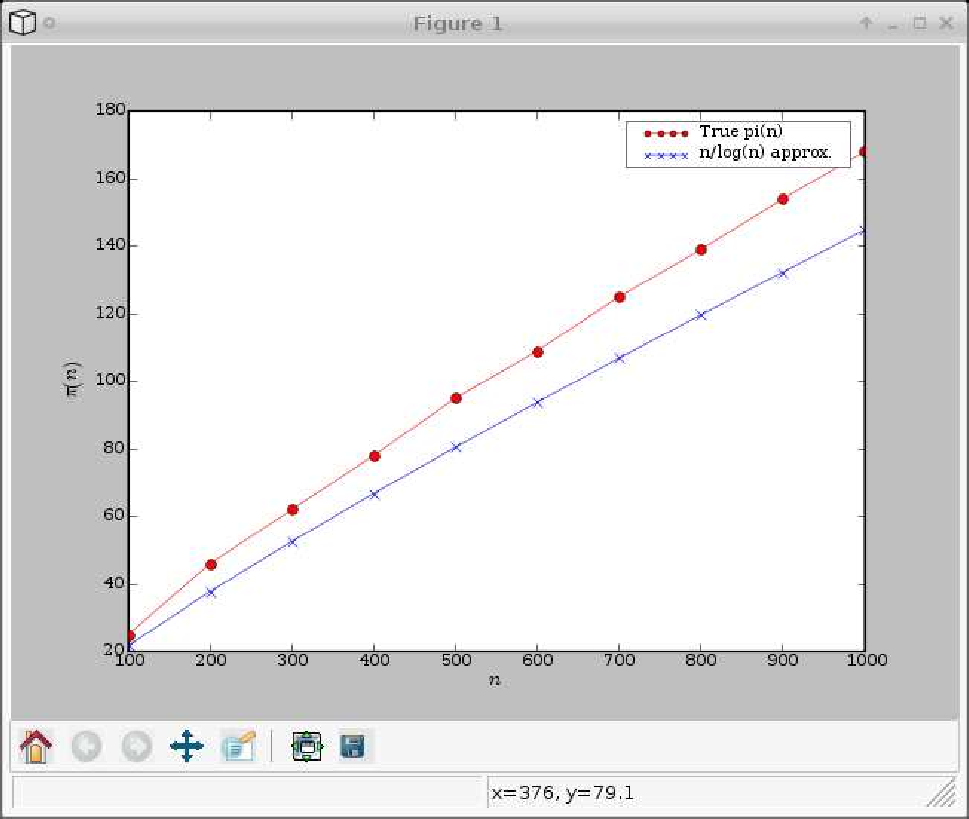
\includegraphics[width=0.85\textwidth,keepaspectratio]{plotExResult} 
    \caption{Gr�fica resultado de la ejecuci�n del ejemplo $\pi$ de Euler}\label{fig:plotExResult}
  
  \end{figure}\end{center}

\paragraph{RSA y paralelismo}
Lorem ipsum\newline
\begin{lstlisting}[captionpos=b,basicstyle=\small,frame=shadowbox,rulesepcolor=\color{black},language=python,caption=$\pi$ de Euler] 
from Client import *
def getKeyPair(keySize):
  " Returns the pair (public, private) keys"
  (p,q) = runInParallel(["result=getPrime(%d)" % keySize ]*2,
      2, 
      "Generating prime pair (p,q)")
  n = p*q
  phi = (p-1)*(q-1)
  while True:
    e = getRandomZLessThan(n)
    if str(gcd(e,phi)) == '1':
      break
  d = modInverse(e,phi)
  return ((e,n) , (d,n))

def cypher(key, msg):
  e = key[0]
  n = key[1]
  return modExp(msg,e,n)

def decypher(key, cyphertext):
  d = key[0]
  n = key[1]
  return modExp(cyphertext,d,n)
\end{lstlisting}


\paragraph{Generadores y $\pi$}
Lorem ipsum\newline
\begin{lstlisting}[captionpos=b,basicstyle=\small,frame=shadowbox,rulesepcolor=\color{black},language=python,caption=$\pi$ de Euler] 
from Client import *

def pi_series():
  sum = R('0')
  i = R('1.0')
  j = R('1')
  four = R("4")
  two = R("2")
  minusOne = R("-1")
  while(1):
    sum += j/i
    yield four*sum
    i += two; j *= minusOne

def euler_accelerator(g):
  s0 = g.next() # Sn-1
  s1 = g.next() # Sn
  s2 = g.next() # Sn+1
  two = R("2")
  while 1:
    yield s2 - ((s2 - s1)*(s2-s1))/(s0 - two*s1 + s2)
    s0, s1, s2 = s1, s2, g.next()

def firstn(g, n):
  for i in range(n):
    yield g.next()
    
\end{lstlisting}



\section{Evaluaci�n}


\section{Conclusiones}
 
  

% EJEMPLOS
\chapter{Ejemplos}

\begin{flushright}
  \begin{minipage}[t]{13cm}
    \begin{flushright}
      \begin{quote}
        \emph{
          Lo mejor para ser escuchados consiste en proporcionar ejemplos claros
        }
        \begin{flushright}
          \textbf{\textemdash Jean Rostand}
        \end{flushright}
      \end{quote}
    \end{flushright}
  \end{minipage}
\end{flushright}

\bigskip

\begin{center}{\line(1,0){325}}\end{center}

%--------------------------------------------------------%

 
\section{Enteros $\mathbb{Z}M_n$}\label{ejZM_n}



% CAPITULO SOBRE LAS POSIBLES MEJORAS, AMPLIACIONES Y CRITICA

\chapter{Cr�tica}

\begin{flushright}
  \begin{minipage}[t]{13cm}
    \begin{flushright}
      \begin{quote}
        \emph{
          Become addicted to constant and never-ending self improvement.
        }
        \begin{flushright}
          \textbf{\textemdash Anthony J. D'Angelo, The College Blue Book}
        \end{flushright}
      \end{quote}
    \end{flushright}
  \end{minipage}
\end{flushright}

\begin{center}{\line(1,0){325}}\end{center}

%--------------------------------------------------------%

\section{Posibles mejoras}
  \subsection{Mayor aprovechamiento de instrucciones SIMD}
    En las operaciones con matrices.

\section{Ampliaciones}
  \subsection{Sobre Polinomios}
    \subsubsection{Factorizaci�n}
      Al igual que para la factorizaci�n de enteros, no se conoce
      un m�todo que permita realizar esta operaci�n en un tiempo razonable. Como es habitual
      en este contexto, �razonable� suele traducirse como �computable en tiempo polinomial�.
      %TODO
  \subsection{Sobre cuerpos finitos}
    En la implementaci�n actual los cuerpos finitos $\GF{p^n}$, 
    se modela $p$ como un entero de tipo \texttt{mpplas::Z}; es decir,
    un entero de precisi�n arbitraria. En la mayor�a de los casos, la caracter�stica de la precisi�n arbitraria
    no es explotada, y de hecho influye negativamente en el rendimiento. De hecho, es usual el uso de cuerpos
    finitos de la forma $\GF{2^n}$. En este caso, es posible explotar el car�cter binario de los elementos.
    Por ejemplo, la suma se reduce a una operaci�n o-exclusivo a nivel de bits. 

    En cualquier caso, la presente biblioteca se centra entorno a tipos de precisi�n arbitraria, raz�n por la cual
    esta caracter�stica tendr�a m�s cabida en otro tipo de biblioteca.


\section{Conclusiones}
  


%% PRUEBAS BORRADOR

\chapter{Pruebas, \textbf{BORRADOR}}
\section{Casos de prueba por funci�n}
\begin{itemize}
  \item divMP(vector, vector)
    \begin{itemize}
      \item[-] Ejemplo: Un entero igual a
        $79228162514264337593543950336 = 2^{32+64}$ y otro igual a 
        $4294967296 = 2^{32}$. Su divisi�n provoca a fecha 21 de Enero 
        que falle la divisi�n debido a que el tama�o del dividendo 
        disminuye m�s r�pido que de uno en uno, mientras que la guarda
        del bucle ``principal'' disminuye de uno en uno.\\
        \textbf{Soluci�n}: La guarda del bucle debe actualizarse en
        funci�n de la variaci�n de tama�o del dividendo.
    \end{itemize}
\end{itemize}

        
        

%%%%%%%%%%%%%%%%%%%%%%%%%%%%%%%%%%%%%%%%%%%%%%%%%%%%%

\bibliographystyle{proyecto}
\bibliography{bibliografia}

\printindex 

\end{document}
